%  A simple AAU report template.
%  2013-03-06 v. 1.0.0
%  Copyright 2010-2013 by Jesper Kjær Nielsen <jkn@es.aau.dk>
%
%  This is free software: you can redistribute it and/or modify
%  it under the terms of the GNU General Public License as published by
%  the Free Software Foundation, either version 3 of the License, or
%  (at your option) any later version.
%
%  This is distributed in the hope that it will be useful,
%  but WITHOUT ANY WARRANTY; without even the implied warranty of
%  MERCHANTABILITY or FITNESS FOR A PARTICULAR PURPOSE.  See the
%  GNU General Public License for more details.
%
%  You can find the GNU General Public License at <http://www.gnu.org/licenses/>.
%
%  A simple AAU report template.
%  2013-03-06 v. 1.0.0
%  Copyright 2010-2013 by Jesper Kjær Nielsen <jkn@es.aau.dk>
%
%  This is free software: you can redistribute it and/or modify
%  it under the terms of the GNU General Public License as published by
%  the Free Software Foundation, either version 3 of the License, or
%  (at your option) any later version.
%
%  This is distributed in the hope that it will be useful,
%  but WITHOUT ANY WARRANTY; without even the implied warranty of
%  MERCHANTABILITY or FITNESS FOR A PARTICULAR PURPOSE.  See the
%  GNU General Public License for more details.
%
%  You can find the GNU General Public License at <http://www.gnu.org/licenses/>.
%
\documentclass[11pt,twoside,a4paper,openright]{report}
%%%%%%%%%%%%%%%%%%%%%%%%%%%%%%%%%%%%%%%%%%%%%%%%
% Language, Encoding and Fonts
% http://en.wikibooks.org/wiki/LaTeX/Internationalization
%%%%%%%%%%%%%%%%%%%%%%%%%%%%%%%%%%%%%%%%%%%%%%%%
% Select encoding of your inputs. Depends on
% your operating system and its default input
% encoding. Typically, you should use
%   Linux  : utf8 (most modern Linux distributions)
%            latin1     
%   Windows: ansinew
%            latin1 (works in most cases)
%   Mac    : applemac
% Notice that you can manually change the input
% encoding of your files by selecting "save as"
% an select the desired input encoding. 
\usepackage[utf8]{inputenc}
% Make latex understand and use the typographic
% rules of the language used in the document.
\usepackage[danish,english]{babel}
% Use the vector font Latin Modern which is going
% to be the default font in latex in the future.
\usepackage{lmodern}
% Choose the font encoding
\usepackage[T1]{fontenc}
%%%%%%%%%%%%%%%%%%%%%%%%%%%%%%%%%%%%%%%%%%%%%%%%
% Graphics and Tables
% http://en.wikibooks.org/wiki/LaTeX/Importing_Graphics
% http://en.wikibooks.org/wiki/LaTeX/Tables
% http://en.wikibooks.org/wiki/LaTeX/Colors
%%%%%%%%%%%%%%%%%%%%%%%%%%%%%%%%%%%%%%%%%%%%%%%%
% load a colour package
\usepackage[table,xcdraw]{xcolor}
\definecolor{aaublue}{RGB}{33,26,82}% dark blue
% The standard graphics inclusion package
\usepackage{graphicx}
\graphicspath{ {figures/Images} }
% Set up how figure and table captions are displayed
\usepackage{caption}
\captionsetup{%
  font=footnotesize,% set font size to footnotesize
  labelfont=bf % bold label (e.g., Figure 3.2) font
}
% Make the standard latex tables look so much better
\usepackage{array,booktabs}
% Enable the use of frames around, e.g., theorems
% The framed package is used in the example environment
\usepackage{framed}
\usepackage{color}
%%%%%%%%%%%%%%%%%%%%%%%%%%%%%%%%%%%%%%%%%%%%%%%%
% Mathematics
% http://en.wikibooks.org/wiki/LaTeX/Mathematics
%%%%%%%%%%%%%%%%%%%%%%%%%%%%%%%%%%%%%%%%%%%%%%%%
% Defines new environments such as equation,
% align and split 
\usepackage{amsmath}
% Adds new math symbols
\usepackage{amssymb}
% Use theorems in your document
% The ntheorem package is also used for the example environment
% When using thmmarks, amsmath must be an option as well. Otherwise \eqref doesn't work anymore.
\usepackage[framed,amsmath,thmmarks]{ntheorem}

%%%%%%%%%%%%%%%%%%%%%%%%%%%%%%%%%%%%%%%%%%%%%%%%
% Page Layout
% http://en.wikibooks.org/wiki/LaTeX/Page_Layout
%%%%%%%%%%%%%%%%%%%%%%%%%%%%%%%%%%%%%%%%%%%%%%%%
% Change margins, papersize, etc of the document
\usepackage[
  left=28mm,% left margin on an odd page
  right=41mm,% right margin on an odd page
  ]{geometry}
% Modify how \chapter, \section, etc. look
% The titlesec package is very configureable
\usepackage{titlesec}
\titleformat*{\section}{\normalfont\Large\bfseries\color{aaublue}}
\titleformat*{\subsection}{\normalfont\large\bfseries\color{aaublue}}
\titleformat*{\subsubsection}{\normalfont\normalsize\bfseries\color{aaublue}}

% Change the headers and footers
\usepackage{fancyhdr}
\pagestyle{fancy}
\fancyhf{} %delete everything
\renewcommand{\headrulewidth}{0pt} %remove the horizontal line in the header
\fancyhead[RE]{\color{aaublue}\small\nouppercase\leftmark} %even page - chapter title
\fancyhead[LO]{\color{aaublue}\small\nouppercase\rightmark} %uneven page - section title
\fancyhead[LE,RO]{\thepage} %page number on all pages
% Do not stretch the content of a page. Instead,
% insert white space at the bottom of the page
\raggedbottom
% Enable arithmetics with length. Useful when
% typesetting the layout.
\usepackage{calc}

%%%%%%%%%%%%%%%%%%%%%%%%%%%%%%%%%%%%%%%%%%%%%%%%
% Bibliography
% http://en.wikibooks.org/wiki/LaTeX/Bibliography_Management
%%%%%%%%%%%%%%%%%%%%%%%%%%%%%%%%%%%%%%%%%%%%%%%%
% Add the \citep{key} command which display a
% reference as [author, year]
\usepackage[square]{natbib}
% Appearance of the bibliography
\bibliographystyle{unsrtnat}
\bibpunct{[}{]}{;}{n}{,}{,}

%%%%%%%%%%%%%%%%%%%%%%%%%%%%%%%%%%%%%%%%%%%%%%%%
% Misc
%%%%%%%%%%%%%%%%%%%%%%%%%%%%%%%%%%%%%%%%%%%%%%%%
% Add bibliography and index to the table of
% contents

\usepackage[nottoc]{tocbibind}
% Add the command \pageref{LastPage} which refers to the
% page number of the last page
\usepackage[
%  disable, %turn off todonotes
  colorinlistoftodos, %enable a coloured square in the list of todos
  textwidth=\marginparwidth, %set the width of the todonotes
  textsize=scriptsize, %size of the text in the todonotes
  ]{todonotes}
% added by KK (ShareLaTeX team)
\usepackage{lastpage}

%%%%%%%%%%%%%%%%%%%%%%%%%%%%%%%%%%%%%%%%%%%%%%%%
% Hyperlinks
% http://en.wikibooks.org/wiki/LaTeX/Hyperlinks
%%%%%%%%%%%%%%%%%%%%%%%%%%%%%%%%%%%%%%%%%%%%%%%%
% Enable hyperlinks and insert info into the pdf
% file. Hypperref should be loaded as one of the 
% last packages
\usepackage{pdfpages}
\usepackage{hyperref}
\hypersetup{%
	pdfpagelabels=true,%
	plainpages=false,%
	pdfauthor={Author(s)},%
	pdftitle={Title},%
	pdfsubject={Subject},%
	bookmarksnumbered=true,%
	colorlinks,%
	citecolor=aaublue,%
	filecolor=aaublue,%
	linkcolor=black,% you should probably change this to black before printing
	urlcolor=aaublue,%
	pdfstartview=FitH%
}

\usepackage[export]{adjustbox}
\usepackage{ragged2e}

\usepackage{listings}
\definecolor{bluekeywords}{rgb}{0,0,1}
\definecolor{greencomments}{rgb}{0,0.5,0}
\definecolor{xmlcomments}{rgb}{0.5,0.5,0.5}
\definecolor{types}{rgb}{0.17,0.57,0.68}
\definecolor{brightpink}{rgb}{1.0, 0.0, 0.5}
\definecolor{midnightred}{rgb}{0.75,0.0,0.0}
\definecolor{blue}{rgb}{0.0, 0.0, 1.0}
\definecolor{caribbeangreen}{rgb}{0.0, 0.8, 0.6}
\definecolor{carrotorange}{rgb}{0.93, 0.57, 0.13}
\definecolor{darkorange}{rgb}{1.0, 0.55, 0.0}
\definecolor{deepcarrotorange}{rgb}{0.91, 0.41, 0.17}
\lstdefinestyle{gglang}{
    language=C,
    basicstyle=\ttfamily\scriptsize,
    keywords=[1]{for,if,while,else,elseif,
			  end, set, to, break,return,case,
			  switch,function, int, double, then, long, decimal, this, void, public, protected, static, private, true, false, func, downto, upto, dcl, of, do},
    keywordstyle=[1]\color{bluekeywords},
    keywords=[2]{Sprite, Game, Math, Time},
    keywordstyle=[2]\color{caribbeangreen},
    keywords=[3]{num, text, bool, point, vector2, list},
    keywordstyle=[3]\color{midnightred},
    commentstyle=\color{greencomments},
    stringstyle=\color{deepcarrotorange},
    showstringspaces=false,
    numbers=left, 
    numberstyle=\tiny,
    extendedchars=true,
    columns=flexible,
    breaklines, breakatwhitespace=true,
    frame=single,
}
\lstset{language=C, style=gglang}

\lstdefinestyle{emolang}{
    language=C,
    keywords=[1]{anus},
    keywordstyle=[1]\color{black},
    keywords=[2]{cutting},
    keywordstyle=[2]\color{black},
    keywords=[3]{cry},
    keywordstyle=[3]\color{black},
    commentstyle=\color{black},
    stringstyle=\color{black},
    showstringspaces=false,
    numbers=none, 
    numberstyle=\tiny,
    extendedchars=true,
    columns=flexible,
    breaklines, breakatwhitespace=true,
    frame=single,
}
\usepackage{float}
% Used for more compact items with \begin{itemize}[noitemsep,nolistsep]
\usepackage{enumitem}
\usepackage{verbatim}
\usepackage{stmaryrd}
\usepackage{pbox}% package inclusion and set up of the document
% see, e.g., http://en.wikibooks.org/wiki/LaTeX/Formatting#Hyphenation
% for more information on word hyphenation
\hyphenation{ex-am-ple hy-phen-a-tion short}
\hyphenation{long la-tex}
% 
%  A simple AAU report template.
%  2013-03-06 v. 1.0.0
%  Copyright 2010-2013 by Jesper Kjær Nielsen <jkn@es.aau.dk>
%
%  This is free software: you can redistribute it and/or modify
%  it under the terms of the GNU General Public License as published by
%  the Free Software Foundation, either version 3 of the License, or
%  (at your option) any later version.
%
%  This is distributed in the hope that it will be useful,
%  but WITHOUT ANY WARRANTY; without even the implied warranty of
%  MERCHANTABILITY or FITNESS FOR A PARTICULAR PURPOSE.  See the
%  GNU General Public License for more details.
%
%  You can find the GNU General Public License at <http://www.gnu.org/licenses/>.
%
%
%
% see, e.g., http://en.wikibooks.org/wiki/LaTeX/Customizing_LaTeX#New_commands
% for more information on how to create macros

%%%%%%%%%%%%%%%%%%%%%%%%%%%%%%%%%%%%%%%%%%%%%%%%
% Macros for the titlepage
%%%%%%%%%%%%%%%%%%%%%%%%%%%%%%%%%%%%%%%%%%%%%%%%
%Creates the aau titlepage
\newcommand{\aautitlepage}[3]{%
  {
    %set up various length
    \ifx\titlepageleftcolumnwidth\undefined
      \newlength{\titlepageleftcolumnwidth}
      \newlength{\titlepagerightcolumnwidth}
    \fi
    \setlength{\titlepageleftcolumnwidth}{0.5\textwidth-\tabcolsep}
    \setlength{\titlepagerightcolumnwidth}{\textwidth-2\tabcolsep-\titlepageleftcolumnwidth}
    %create title page
    \thispagestyle{empty}
    \noindent%
    \begin{tabular}{@{}ll@{}}
      \parbox{\titlepageleftcolumnwidth}{
        \iflanguage{danish}{%
          
\includegraphics[width=\titlepageleftcolumnwidth]{resources/Logos/aau_logo_da}
        }{%
          
\includegraphics[width=\titlepageleftcolumnwidth]{resources/Logos/aau_logo_en}
        }
      } &
      \parbox{\titlepagerightcolumnwidth}{\raggedleft\sf\small
        #2
      }\bigskip\\
       #1 &
      \parbox[t]{\titlepagerightcolumnwidth}{%
      \textbf{Abstract:}\bigskip\par
        \fbox{\parbox{\titlepagerightcolumnwidth-2\fboxsep-2\fboxrule}{%
          #3
        }}
      }\\
    \end{tabular}
    \vfill
    \iflanguage{danish}{%
      \noindent{\footnotesize\emph{Rapportens indhold er frit tilgængeligt, men offentliggørelse (med kildeangivelse) må kun ske efter aftale med forfatterne.}}
    }{%
      \noindent{\footnotesize\emph{The content of this report is freely available, but publication (with reference) may only be pursued due to agreement with the author.}}
    }
    \clearpage
  }
}

%Create english project info
\newcommand{\englishprojectinfo}[8]{%
  \parbox[t]{\titlepageleftcolumnwidth}{
    \textbf{Title:}\\ #1\bigskip\par
    \textbf{Theme:}\\ #2\bigskip\par
    \textbf{Project Period:}\\ #3\bigskip\par
    \textbf{Project Group:}\\ #4\bigskip\par
    \textbf{Participant(s):}\\ #5\bigskip\par
    \textbf{Supervisor(s):}\\ #6\bigskip\par
    \textbf{Copies:} #7\bigskip\par
    \textbf{Page Numbers:} \pageref{LastPage}\bigskip\par
    \textbf{Date of Completion:}\\ #8
  }
}

%Create danish project info
\newcommand{\danishprojectinfo}[8]{%
  \parbox[t]{\titlepageleftcolumnwidth}{
    \textbf{Titel:}\\ #1\bigskip\par
    \textbf{Tema:}\\ #2\bigskip\par
    \textbf{Projektperiode:}\\ #3\bigskip\par
    \textbf{Projektgruppe:}\\ #4\bigskip\par
    \textbf{Deltager(e):}\\ #5\bigskip\par
    \textbf{Vejleder(e):}\\ #6\bigskip\par
    \textbf{Oplagstal:} #7\bigskip\par
    \textbf{Sidetal:} \pageref{LastPage}\bigskip\par
    \textbf{Afleveringsdato:}\\ #8
  }
}

%%%%%%%%%%%%%%%%%%%%%%%%%%%%%%%%%%%%%%%%%%%%%%%%
% An example environment
%%%%%%%%%%%%%%%%%%%%%%%%%%%%%%%%%%%%%%%%%%%%%%%%
\theoremheaderfont{\normalfont\bfseries}
\theorembodyfont{\normalfont}
\theoremstyle{break}
\def\theoremframecommand{{\color{aaublue!50}\vrule width 5pt \hspace{5pt}}}
\newshadedtheorem{exa}{Example}[chapter]
\newenvironment{example}[1]{%
		\begin{exa}[#1]
}{%
		\end{exa}
}

%todo
\newcommand\myworries[1]{\todo[red]{#1}}
%\renewcommand\todo[1]{} %Kommentér ud for at vise todos

%Short Cuts
\newcommand{\lang}{BFGL}

%for making operational semantics by Giovanni
\newcommand{\transE}[5][\mathit{env}_V]{ #1 \vdash \langle #2 , #3 \rangle \to_e (#4 , #5)  }
%$$ 
%\transE[\mathit{env}_V, \mathit{env}_F]{e}{sto}{v}{sto'}
%$$
% my new macros
\usepackage[parfill]{parskip}

\begin{document}
%frontmatter
\pagestyle{empty} %disable headers and footers
\pagenumbering{roman} %use roman page numbering in the frontmatter
%  A simple AAU report template.
%  2013-03-06 v. 1.0.0
%  Copyright 2010-2013 by Jesper Kjær Nielsen <jkn@es.aau.dk>
%
%  This is free software: you can redistribute it and/or modify
%  it under the terms of the GNU General Public License as published by
%  the Free Software Foundation, either version 3 of the License, or
%  (at your option) any later version.
%
%  This is distributed in the hope that it will be useful,
%  but WITHOUT ANY WARRANTY; without even the implied warranty of
%  MERCHANTABILITY or FITNESS FOR A PARTICULAR PURPOSE.  See the
%  GNU General Public License for more details.
%
%  You can find the GNU General Public License at <http://www.gnu.org/licenses/>.
%
\pdfbookmark[0]{Front page}{label:frontpage}%
\begin{titlepage}
  \addtolength{\hoffset}{0.5\evensidemargin-0.5\oddsidemargin} %set equal margins on the frontpage - remove this line if you want default margins
  \noindent%
  \begin{tabular}{@{}p{\textwidth}@{}}
    \toprule[2pt]
    \midrule
    \vspace{0.2cm}
    \begin{center}
    \Huge{\textbf{
     Design and implementation of \lang{} % insert your title here
    }}
    \end{center}
    \begin{center}
      \Large{
        - Beginner Friendly Game Language -% insert your subtitle here
      }
    \end{center}
    \vspace{0.2cm}\\
    \midrule
    \toprule[2pt]
  \end{tabular}
  \vspace{4 cm}
  \begin{center}
    {\large
      Project Report%Insert document type (e.g., Project Report)
    }\\
    \vspace{0.2cm}
    {\Large
      ds405f16%Insert your group name or real names here
    }
  \end{center}
  \vfill
  \begin{center}
  Aalborg University\\
  Department of Computer Science\\
  Selma Lagerlöfs Vej\\
  DK-9220 Aalborg
  \end{center}
\end{titlepage}
\clearpage
\listoftodos
\thispagestyle{empty}
{\small
\strut\vfill % push the content to the bottom of the page
\noindent Copyright \copyright{} Aalborg University 2016\par
\vspace{0.2cm}
\clearpage


\pdfbookmark[0]{English title page}{label:titlepage_en}
\aautitlepage{%
  \englishprojectinfo{
    Design and implementation of BFGL %title
  }{%
    Design, definition and implementation of programming languages %theme
  }{%
    Spring Semester 2016 %project period
  }{%
    sw405f16 % project group
  }{%
    %list of group members
August Malling Kørvell\\
Carsten Ibsen\\
Mathias Leding\\
Kristoffer Mathiasen Degn\\
  }{%
    %list of supervisors
   Giovanni Bacci 
  }{%
    1 % number of printed copies
  }{%
    \today % date of completion
  }%
}{%department and address
  \textbf{Selma Lagerlöfs Vej}\\
9220 Aalborg Ø\\
Denmark\\
  \href{http://cs.aau.dk}{http://cs.aau.dk}
}{% the abstract
The computer science industry is growing rapidly, and to be able to meet the increased demand for computer scientists and engineers alike, it is essential that the numbers of students within the field grows at an equally increasing rate. A way to try and accomplish this, is to spark an interest in computers and programming from an early age. In this report, the authors tries to do this by designing and implementing a programming language designed to teach young people about programming through the development of something they know and care about: Video games.

The language is designed to be as beginner friendly as possible. An example of how this is done, is that the language design aims to replace symbols with words. To make the user experience focused on actually writing code, as opposed to learning how to use a complicated IDE, a simple graphical user interface has been developed for the \lang{} compiler.

A language specification was written and a corresponding compiler was made.
}


\cleardoublepage
\pdfbookmark[0]{Contents}{label:contents}
\pagestyle{fancy} %enable headers and footers again
\tableofcontents
\chapter*{Preface\markboth{Preface}{Preface}}\label{ch:preface}
\addcontentsline{toc}{chapter}{Preface}
%Here is the preface. You should put your signatures at the end of the preface.

\vspace{\baselineskip}\hfill Aalborg University, \today
\noindent

This report is worked out by August M. Kørvell, Carsten Ibsen, Kristoffer M. Degn and Mathias J. B. Leding from SW405f16 on Aalborg University. This report was done in the span of 4 months from February to May 2016 to make a programming language targeted at young people. The purpose of the report is to make a simple programming language for beginners to not scare away potential programmers. The authors behind this report would like to thank Klaus Kørvell for providing the source of the curriculum of 9. graders in Denmark \cite{FFMM}. Furthermore, a huge thanks to Giovanni Bacci for an outstanding work as supervisor.
\vfill \vfill


\begin{minipage}[b]{0.45\textwidth}
 \centering
 \rule{\textwidth}{0.5pt}\\
  August Malling Kørvell\\
 {\footnotesize <akarve14@student.aau.dk>}
\end{minipage}
\hfill
\begin{minipage}[b]{0.45\textwidth}
 \centering
 \rule{\textwidth}{0.5pt}\\
  Carsten Ibsen\\
 {\footnotesize <cibsen13@student.aau.dk>}
\end{minipage}
\hfill
\vspace{3\baselineskip}
\vfill\noindent
\begin{minipage}[b]{0.45\textwidth}
 \centering
 \rule{\textwidth}{0.5pt}\\
  Mathias Leding\\
 {\footnotesize <mledin14@student.aau.dk>}
\end{minipage}
\hfill
%\vspace{3\baselineskip}\vfill\noindent
\begin{minipage}[b]{0.45\textwidth}
 \centering
 \rule{\textwidth}{0.5pt}\\
  Kristoffer Mathiasen Degn\\
 {\footnotesize <kdegn14@student.aau.dk>}
\end{minipage}
\hfill

\cleardoublepage
%mainmatter
\pagenumbering{arabic} %use arabic page numbering in the mainmatter
\chapter{Introduction}
\begin{comment}
1. To whom is this a problem? (i.e., who is going to benefit from your solution?)
Society in general. According to http://www.sitepoint.com/6-reasons-why-your-child-and-mine-should-learn-to-code, there will be 1 million unfilled jobs in programming/IT by 2020 if nothing is done.

2. Why is this a problem? (motivate why you believe this is an interesting problem)
It is a problem because the IT industry is growing rapidly, and has been ever since the invention of computers. The amount of people getting an education related to programming is not enough to cover the needs of the world. One way to remedy this, is to teach children programming at an early age, or at least to get them interested in it. We already have things like Scratch, but the step from that and into a real programming language like Java or C\# can be a daunting challenge for many kids. Therefore, we think it could be interesting to develop a language that lands somewhere in between Scratch and a real language. 

3. How do you plan to solve this problem? (sketch a preliminary problem Analysis, listing the techniques you think will be used in this project)
We plan to take a look at different programming languages for kids that already exist, like Scratch, and see if we can hit an abstraction level somewhere in between tools like Scratch, and a real programming language. We want to focus the language on creating simple 2D games, as this will help getting more children interested in programming. 
We will implement the language by compiling it to Java, so that we can use the game library Slick2D.


In our modern society, everything is controlled by computers. Most people, in the western world, interact directly with a computer every day, and many even carry one with them, namely their smartphone. However, as technology becomes a more integrated part of our lives, more and more abstraction layers are created to distinct the user from the 'machinery'.

The consequences of this is that there is a much greater need to understand, not only how to use these devices, but also how to utilise them in new and innovative ways. Furthermore, the IT industry has been growing at increasingly faster rates, and nothing indicates that it is going to slow down any time soon. It is therefore important to educate more people in the field of computer science.

A method to reach this, is to try and invoke an interest in the field early on, by introducing children to programming. Since a lot of children have an interest in video games, we believe that this can help to develop this wanted interest, by giving them the opportunity to create their own video games with basic tools. Furthermore, it is more motivating to be able to create graphics and make it react to what you type, rather than just seeing some text in a terminal window.








it is not needed to be able to write code but just the way of thinking behind it. This can give a lot of benefits to children and adults in the way they approach a problem, where they have a big problem that they keep on making into smaller and smaller problems so they end up with having a lot of small and easy-to-understand problems, or the way they work around a problem with lot more logical approach. 

\end{comment}




In our modern society, everything is controlled by computers. Most people, in the western world, interact directly with a computer every day, and many even carry one with them, namely their smartphone\citep{geny}. However, as technology becomes a more integrated part of the everyday life, more and more abstraction layers are created to distinct the user from the inner workings of the technology.

The consequences of this is that there is a much greater need to understand, not only how to use these devices, but also how to utilise them in new and innovative ways. Furthermore, the IT industry has been growing at increasingly faster rates and nothing indicates that it is going to slow down any time soon \citep{BLSGrowth}. It is therefore important to educate more people in the field of computer science.

A way to achieve this, is to try and invoke an interest in the field early on, by introducing young people to programming. Since a lot of young people have an interest in video games, this would be a good approach to try and invoke this interest. An example of people doing this is found on Code.org\citep{codeorg}. This company believes that teaching coding via games can help children to develop an interest in programming, by giving them the opportunity to create their own video games using basic tools. Furthermore, it can be more motivating to be able to create graphics and make it react to user input, rather than just seeing some text in a terminal window.

Even though only some will develop an interest for computer science, having the ability to understand how programs work can be very beneficial. The goal is not to teach people all the necessary skills to make a whole program, but to introduce them to the logical thinking that is at the core of programming and writing code in general. \citep{Sitepoint2015}


Building on this, in this report, a programming language will be designed, for use in an educational context.
\chapter{Preliminary analysis}


This chapter will analyse existing tools and programming languages that can be used to introduce young people to programming, as well as the fundamentals of game development, to better understand how to design a new programming language that can assist in introducing and engage young people to programming and computer science in general. At the end of this chapter, a problem statement will be defined as a basis for the language that will be designed later in this report.

\section{Beginner friendly programming}
A lot of programming languages can be difficult to use for children and users with little to no experience in programming, as they are not used to the large amount of symbols, the logic behind control flow statements, and the even larger amount of keywords.

This chapter will therefore examine some of the characteristics that are needed for a language to be beginner friendly, both in terms of language design, but also in terms of what kind of, if any, Integrated Development Environment (IDE) should be provided with the language compiler.
An obvious example of an easy-to-learn for beginners language could be Scratch\cite{scratch}, which has an online IDE and compiler on one page. A great part of the success of Scratch comes from exactly that - the integrated IDE/compiler - which is incredibly easy for a kid to use.
Some widely used programming languages are not as beginner friendly as Scratch. Take for example this piece of code in Scheme:
\begin{figure}[H]
    \centering
    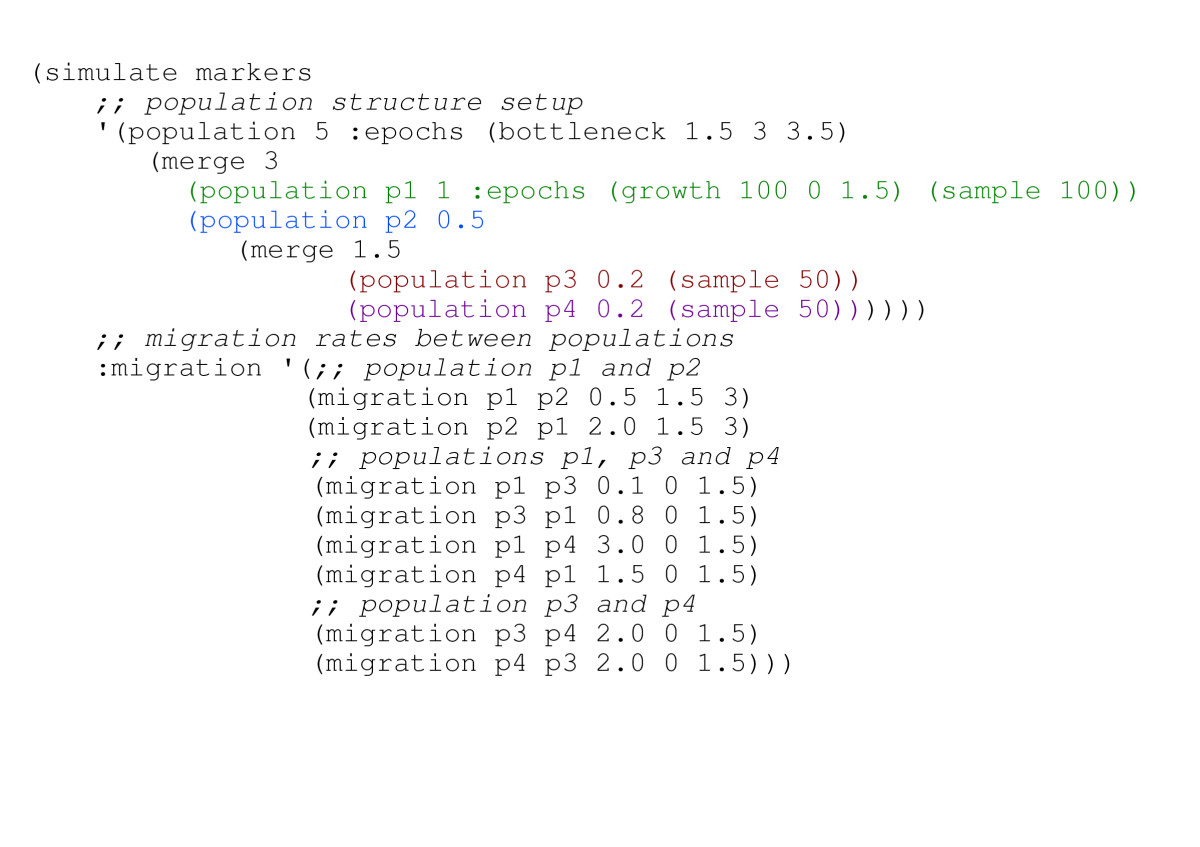
\includegraphics{resources/Images/schemes***.png}
    \caption{This example is supposed to function like a basic for-loop. It does something ten times.}\cite{Schemeexample}\label{fig:schemestuff}
\end{figure}

To the untrained eye, this will seem confusing. The keywords are not inherently easy to understand, and there are numbers/other symbols dispersed all over the code. Furthermore, the amount of parenthesis can easily confuse the user, as it is not clear which parenthesis belongs together, or even why they are there in the first place.

\subsection{Beginner friendly language design}
When making a language beginner friendly, there are a couple of things that should be taken into account. This section talks about the importance of keywords, dynamic and static typing, syntax structure, and type simplicity.
\subsubsection{Keywords}
The meaning (semantics) of a keyword should be readily seen, and intuitive when it is initially looked at. For example, the \textit{namespace} keyword in C\# can be used to declare a scope which can contain a collection of related objects. The objects could for example all belong to the same application, or maybe the same framework. It can be compared to sets in the mathematical fields, which is a collection of related symbols. Namespaces are a very common concept within programming and other computer related fields, but outside that, it is not really widely used or understood. Young users of programming languages will probably not have encountered the word before, and as such, it will contribute to the confusion of learning a new language. If instead of "namespace", something like "scope" or "set" had been used. It would help young users, or users new to programming in general to not be confused when initially learning the language.


\subsubsection{Dynamic and static typing}
Dynamic or static typing is very important for the readability of a language It is therefore important to make the right choice for new users. 
\\Dynamic typing means that a keyword like \textit{var} can be used in C\#, which allows the actual type of a variable to be determined at runtime. This can lead to a lot of confusion when type conversion exceptions are suddenly thrown during execution, because the user realistically has no idea what type of variable actually is in the variable. The upside is that it takes less time to write in this language, as the programmer does not have to think about what type the programmer wants something to be, and what representation of it the programmer wants to use. 
\\Static typing means that the programmer has to use the explicit type they want a variable to be when you are declaring it. This will usually lead to less confusion for inexperienced programmers, as they have to think about what they want a variable to be, and not just remember it based on what they do to that variable. This can however lead to confusing problems when converting between similar types, as for example in c\#, where there are multiple types for number-representation, such as: int, double and decimal. Some conversions between these are allowed, and others are not, which can lead to extra work and confusion when a type suddenly will not fit the input the programmer is giving it.

A language for beginners has to be clear and readable, and this is the main reason that static typing is better for beginners than dynamic typing. If the language is static, the beginner will not have unforeseen conversion errors, or variables that get the wrong input. Of course, cases as the one with multiple representations of numbers in c\# has to be avoided when using static typing. 


\subsubsection{Syntax structure}
When designing a syntax structure that is easy to read for beginners, simplicity is not the main focus, but rather readability. For example in Pascal, all variables has to be declared in the beginning of a function - or procedure as it is called in Pascal:

\lstset{language=[Sharp]C}  
\begin{figure}[H]
\centering
\begin{lstlisting}
procedure DoSomething; 
 var 
  x : Tsome_type;
  y : Tsome_otherType;
  z : Tsome_otherOthertype;
 begin
 if (x > y) then
      z := x
   
   else
      z := x;
   z := z;
 end;
\end{lstlisting}
\caption{Pascal local variable declaration.}\cite{pascalvar}
\label{fig:pascalvar}
\end{figure}
This can lead to somewhat unreadable code, because as it is read, each time a variable is encountered the reader has to go up and look at what kind of variable it is. The upside is that there can never be any doubt about where a variable is declared. A beginner might have a hard time remembering what types all his variables are, and having to go up and look might make it harder to read. 
\\Instead of doing it like in Pascal, it could be done like in Java, which allows variable declaration anywhere:
\lstset{language=[Sharp]C}  
\begin{figure}[H]
\centering
\begin{lstlisting}
public void SomeMethod(){

    int x = 0;
    x = x + 1;
    int y = 100;
    
    public void SomeOtherMethod();
    
    int z = 12;
    x = y+z+x;
    
    public void SomeOtherMethod();
}
\end{lstlisting}
\caption{Pascal local variable declaration.}
\label{fig:javavar}
\end{figure}
This allows variables to be declared where they are needed, and as such, it can improve the readability of the language. The downside of this is that when reading a method, the reader might have to look for a while to find a variable, if it is not properly placed closely to where it is used. 

\subsubsection{Type simplicity}
Keeping the types relatively simple is good for beginners, but only if the meaning of the type is also kept clear. For example, the meaning of \textit{char} in C is relatively clear, but the meaning of something like \textit{struct} is not. \textit{Struct} in itself is rather unintuitive.
So to be usable in a beginner friendly language, types should preferably be kept simple, and without too many different uses. It should not be presumed that beginners inherently know anything about the different constructs in programming. The meaning of a given type needs to be discernible from the type name.
\newpage
\subsection{Beginner friendly tools}
As a beginner, one of the most daunting tasks can be choosing the development environment in which to write code. In some languages, this is taken care of for you. For example in Scratch\cite{scratch}, where the only way to actually "write" in the language is through their website, with a visually based way of defining a program. 
If a beginner was to, for example, start in C\#\cite{CSHARP} and by extension use visual studio, it could be a very confusing experience. Visual studio has a mess of options, toolbars, windows and the like:
\begin{figure}[H]
    \centering
    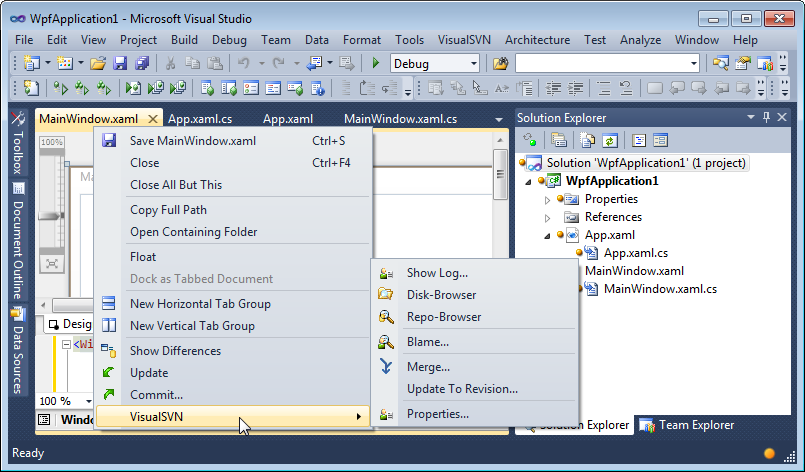
\includegraphics[scale=0.5]{resources/Images/vsclutter.png}
    \caption{Visual Studio clutter}
    \label{fig:vsclutter}
\end{figure}

This is hard to understand without some knowledge of programming beforehand. Therefore, it is useful for a beginner friendly programming language to have some kind of user friendly Interactive Development Environment (IDE) to let the user program in. Otherwise, it is going to be difficult for beginners to get started with programming in the language.
To summarize, it is important that the readability of the language is great when designing for beginners and kids. A more verbose syntax should be preferred over a clean and simple one, like in C\#\cite{CSHARP}, to make the writing of the language closer to actually writing a story, rather than programming a computer to do tasks. Types and keywords have to be intuitive in their use, and the complexity of any given type or keyword cannot be too great, or the readability will suffer from it. Furthermore, the medium in which the language is written is important. A user friendly IDE is paramount to help beginners getting started in a beginner friendly language.
\section{Game development}
In this section, the different components of video game development and how it differs from ordinary application development are analysed. Afterwards, some examples of tools for game development are described, namely \textit{Scratch}, GameMaker and PyGame. This is done to develop a better understanding of which kinds of tools are available to a new developer.

%This section will analyse how games are developed right now, how flow of the project is when you program the game and how this flow can different then a more normal project flow, in a company where you have to make program to some one. after this there will be a look at some of the tools that exist to make this easy for people to program like block programing, here should be look at scratch, then there are combination of block and text programing, here should be look at GameMaker since this still have block program but also text base program in the languge GML(GameMaker Language) and at last only text base programing in this case here should be looked at PyGame this is in python and is a layer over SDL that give easy access to some thing that you need in game develoment.

\subsection{Components of game development}
%To better understand how game development differs from more conventional development, it is important to first understand how to develop a video games.


To develop a video game, the developer needs to manage components that are specific for the domain of game development. All video games must be able to handle user input and have a way to display some sort of output to the user. This output is often in the form of graphics drawn by the graphics card to the screen. Depending on the kind of video game that is being developed, different components are needed. These components include, but are not limited to: 

\begin{itemize}
 \item Collision Detection
 \item Physics
 \item Animation
 \item Graphics (2D and 3D)
 \item Artificial Intelligence
 \item User Input
 \item File Input/Output
 \item Networking \ldots
\end{itemize}

%When developers work on a game they work close together with a team of game designers in bigger companies, they stand for the vision of the game, how they think it should what could be fun the sound the image models and all of those tings you job as the game programmer is to take there's vision and turn it in to realty on the hardware and software you have. and this can be very hard since there so many components in the development of a game, a few things you need to make.\cite{DesignVSPrograming2016}

There are different tools and frameworks that add abstraction layers to game development so that a developer can focus on developing a game, instead of having to spend a lot of time on implementing things like graphics, physics and networking. Some of these tools are described in the following section.

%many of those things can be made easy to understand and use in a program language that is design to make games in, and this will give a faster and better work, and can help introducing new people the programing and game development.

%To answer the question "How is the flow of game development different than programming a normal piece of software?",  \cite{StackGameVSSoftware2011} on a forum post there have been a few people that did talk about their experience in the field of gaming, and how they think it is different, one say that the different lay in the size of the project and a bigger risk and other say that it is the target of what you try to do, when you make a program for a company, you need to make it easy to use and have all the features that ask for, but in the game you need besiege the easy of use also that it is fun to use/play, and that have to think about this under the hole project is he say was the hardes part, and they there where those that say that there were no real different between the two that it was the same thing, so like with software you make for other company's it is something that chance from project to project and is never the same.



\subsection{Existing solutions}
There is a number of tools to develop video games. To best understand the domain, three different tools are described in the following section, namely \textit{Scratch}, \textit{GameMaker} and \textit{PyGame}.
These have been chosen, since they each represent a different approach to video game development.

%In this subsection, three different existing tools with three different approaches are described. The first solution uses block programming only, the second uses both block programming and textual programming, and the third uses textual programming only. This way, \todo{pls help}

\subsubsection{Scratch}
Scratch is a visual programming language, which means that the user programs with a graphical interface rather than a textual one. It utilises block programming instead of actual code. This way, the user does not learn to write code, but rather the mindset of programming. The blocks are conveniently grouped in relevant groups. For example, the group "motion" contains the "move" block, which makes the character move a certain amount of steps, and "turn" blocks, which makes the character turn either clockwise or counterclockwise. By putting these kinds of blocks together, Scratch translates it to actual code.

\begin{figure}[H]
\centering
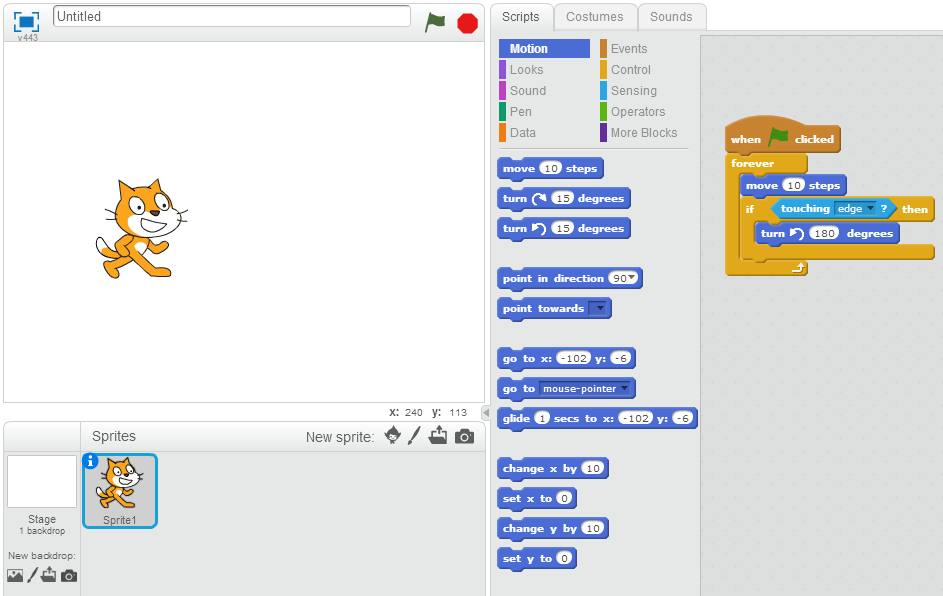
\includegraphics[scale=0.5]{resources/Images/Scratch.png}
\caption{Small program made in Scratch}
\label{fig:Scratch}
\end{figure}

On figure \ref{fig:Scratch} a simple program made in Scratch is seen. This program makes the character indefinitely walk 10 steps in one direction and rotate the character 180 degrees if it hits the wall. The green flag corresponds to running the main function of a conventional programming language.
The easy-to-learn interface and the child friendly design, makes Scratch an ideal solution for the youngest people who wants to be introduced to the world of programming.\cite{scratch}

\subsubsection{GameMaker}
GameMaker is a game making software that implements a mixture of drag and drop programming and their own language called GameMaker Language, which is an interpreted scripting language based on C. This way, it is possible to create games quickly and easily with the drag and drop while at the same time having flexibility and control of conventional programming with GameMaker Language.

\begin{figure}[H]
\centering
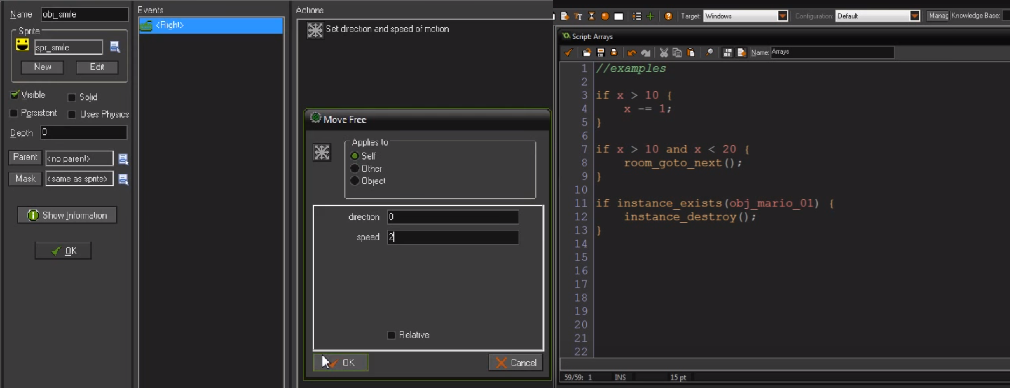
\includegraphics[scale=0.5]{resources/Images/GameMaker.PNG}
\caption{On the left is drag and drop\cite{GMDnD}. On the right is GML \cite{GML}}
\label{fig:GameMaker}
\end{figure}

On figure \ref{fig:GameMaker} an example of the two is shown. On the left is the drag and drop system, where actions gets paired with events. In this example, the right arrow key makes obj\_smile move 2 pixels per frame towards direction 0. On the right side, examples of if-statements in GML are pictured.

\subsubsection{PyGame}
PyGame is a set of Python modules used to make it easier to make games in the programming language Python. This means that it adds a number of functionalities which aid in the game making process. PyGame utilises fully conventional coding and requires the programmer to write actual code.
An example of functionalities is pygame.event.get(), which retrieves every event currently in queue to get handled.

\begin{figure}[H]
\centering
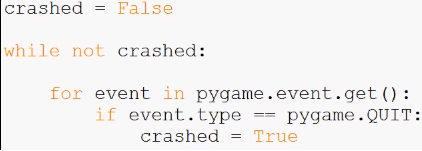
\includegraphics[scale=0.6]{resources/Images/PyGame.png}
\caption{Small PyGame program}
\label{fig:PyGame}
\end{figure}

Figure \ref{fig:PyGame} uses this functionality by checking every event in the queue. Furthermore, it uses pygame.QUIT which is the event type in PyGame that means that the close button has been pressed. Therefore, this code checks every event in the queue if they are a click on the close button. If they are, the program breaks out of the for loop.

\subsection{Target audience}
\label{sub:TargetAudience}
The tools described in this chapter cover a wide spectrum in terms of beginner friendly game development. Scratch\cite{scratch} is easy to use for beginners, and Pygame is meant for more experienced developers. There is, however, a slot somewhere in between Scratch and GameMaker/Pygame, which has to help beginners going from scratch to something like Pygame, and introduce them to control structures, boolean logic, and other concepts of programming. This transition could turn some off from wanting to do more programming, as it may seem too complicated and scary. This is why there is a need for a language in between these two types of programming languages that is simple and easy to learn. Furthermore Scratch looks and feels child-friendly, which is not appealing for a teenager, who wants to be introduced to some less basic concepts of programming while at the same time not getting a lot of advanced and confusing features.

For a textual programming language to have any functionality, it has to use mathematics. These include vectors used in, among others, simulating motion of objects and basic algebra used in variables, which are very essential parts of game development.
As these are an essential part of programming, the target audience has to know, or at least have the preliminary knowledge needed to learn these concepts. As seen in \cite{FFMM} from the Ministry of education, students are introduced to use variables from around the sixth grade in Denmark, but will not learn to use functions and equations before seventh to ninth grade. Therefore, the target audience (TA) is chosen to be students starting from the ninth grade.



With this in mind, there will in the following section be defined a problem statement.
\newpage
\section{Problem statement}
\label{sec:problemstatement}
The goal of this paper is to design and develop a beginner friendly programming language that can help to motivate and introduce young people to programming.

To build upon the knowledge that the end user has about mathematics and logic, as described in \ref{sub:TargetAudience}, and to give them a foothold in the world of programming, some concepts are more appropriate than others, and will therefore be the main focus of the language described in this paper. These concepts are as follows:

\begin{itemize}
    \item Control flow.\\
    This is important for new programmers to understand, since it lies at the root of the most popular programming languages. Having an understanding of control flow, such as if/else constructs can help the user to better understand structured programming.
    
    \item Variables.\\
    As stated in \ref{sub:TargetAudience}, the end user of the language is assumed to have a basic understanding of algebra. This includes simple algebraic problems such as "Find x, when x + 2 = 4". The next natural step, for the user, is to learn about variables, since this may help them to better understand algebra by giving a real life use for it.
    
    \item Object oriented programming.\\
    Having focus on simple object oriented concepts may help the user to understand the mindset of object oriented programming, making it easier to learn a more complex object oriented programming language in the future.
    Furthermore, it is easier to create games with an object oriented language, and it is easier for a beginner to model the program after real life.
    %Having focus on simple object oriented concepts, may help the user to figure out how to write a program, since this can help the user to model the program after what they see in the real world.
\end{itemize}


Since the language described in this paper is designed specifically to aid beginners with developing simple video games, it is advantageous for the language to be domain specific, i.e a domain-specific language (DSL). This way, the end user can focus on developing and designing games instead of worrying about drawing graphics and other technical problems in game design. To attain this, the language should implement common constructs used in game design to apply abstraction layers to the technical part of developing a video game.

From all this, and based on the rest of the analysis, the following problem statement has been defined:

\textit{How can a domain-specific language that can help to motivate and introduce young people to programming, in particular to concepts like control flow, variables and other basic concepts from object oriented programming, be designed and developed, such that the end user can focus on designing and implementing simple games and not worry about the more technical part of game development?}









\chapter{Language Design}
This chapter describes the design of \lang{}. It also contains a mini-tutorial of how to use \lang{} and some informal definitions of parts of the language. 
\section{Language Evaluation Criteria}
In this section the different criteria proposed in \cite{sebesta1.3} are presented. These criteria are used to facilitate the design of \lang{}.
The three main aspects of a language, according to \cite{sebesta1.3}, are \textit{Readability, Writability and Reliability}. These have a list of criteria which is applicable to the main aspects:
\begin{figure}[H]
    \centering
    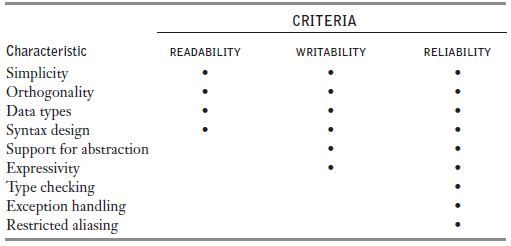
\includegraphics[scale=1]{resources/Images/criteria.PNG}
    \caption{Table from \cite{sebesta1.3} with the different criteria, and how they affect aspects of the language.}\label{fig:Criteria}
\end{figure}
The following sections briefly summarise the aspects covered by the above-mentioned criteria.
\newpage
\subsection{Readability}
An important aspect of a beginner-friendly programming language is that it has to be easily readable. When considering the readability, the problem-domain also has to be drawn in, as a language could be readable when used for writing games, which is the main domain of the language, but difficult to read when used for writing something not in the domain of the language.
\subsubsection{Simplicity}
The simplicity of a language has to take into account 3 important aspects:
\begin{itemize}
    \item \textbf{Language constructs}:\\
     A language with a large amount of constructs can be hard to remember, and in reality, a lot of programmers might learn a subset of the total amount of features of a language, instead of learning the language as a whole.
    \item \textbf{Feature multiplicity}:\\
     Having multiple ways to accomplish the same thing can be confusing and hard to read, especially for beginners. The fact that something can be done in many different ways is bad for the readability, because it might not be what this particular programmer expects to see when he reads a program.
    \item \textbf{Operator overloading}:\\
    One operator symbol meaning multiple things can lead to bad readability. The meaning of operators are typically clear and easy to understand, but if an operator is suddenly overloaded to do something else based on the context, it can become harder to read.
\end{itemize}
\subsubsection{Orthogonality}
Orthogonality means that the ways in which the primitive constructs of the language can be combined together, is relatively small, and the combinations that do exist, are meaningful. This is important when programming, because if the orthogonality is too low, the usage of the different combinations will not make sense to the programmer. This is because too many exceptions in how the programming language works, confuses the programmer, thus making it nonsensical. 
\subsubsection{Syntax Design}
Regarding the design of the syntax of a language, one should take two important aspects into account:
\begin{itemize}
    \item \textbf{Reserved words}:\\
    These constitute words such as:
    \begin{itemize}
        \item \textit{while}
        \item \textit{if}
        \item \textit{for}
    \end{itemize}
    If the reserved word used to do control structures such as these are not named in a meaningful way, the reader may find it difficult to understand the semantics of a piece of code.
    \item \textbf{Form and meaning}:\\
    This sub-criterium refers to the idea that the behavior of the statements should somehow be self-explanatory to aid readability. 
\end{itemize}
\subsubsection{Data Types}
There should be sufficient data types to support most common tasks in programming, as this makes it easier and faster to program, since the programmers do not have to define new types themselves.
\subsection{Writability}
The second important aspect for a beginner friendly language is that it should be easy to write. This does not necessarily mean that it has to be simple or written with few words, but more so that it has to be easy to understand how to write code. This is achieved by fulfilling a number of criteria, listed in the next couple of sections.
\subsubsection{Simplicity and orthogonality}
When beginners begin to learn how to use and write programs in a new language, they will not know all of the different constructs available in the language. This can lead to programs that perform poorly or programs that are simply wrong. This is because the beginners will use the constructs they know, or can intuitively understand, and not the more advanced or unknown ones.
\subsubsection{Support for Abstraction}
It is important in any programming language that there is proper support for abstraction. Otherwise programs in the language are complicated to read. The creation of new programs will take longer, and the maintainability of the programs would become more difficult and error prone. A beginner is not going to be too concerned with maintainability, but the concept of abstraction over certain parts of a program via the use of, among others, methods/subroutines data structures, is a very concept of programming languages in general that a beginner needs to get used to. A language with good support for abstraction will also feel more natural to write in. 
\subsubsection{Expressivity}
This criteria simply refers to the fact that the language should have convenient ways of expressing complex computations.
\subsection{Reliability}
Reliability is about whether or not a program performs how it should under all kinds of conditions. The following sections presents the main aspects that contribute to making a language reliable.
\subsubsection{Type Checking}
A language designed for beginners should have static type checking as opposed to dynamic type checking. Such a language should be designed to guide and help beginners, and having dynamic type checking leaves a lot of type casting errors to be found by the programmer while executing the program. These errors can be particularly hard to debug in advance. 
\subsubsection{Exception Handling}
Exception handling is about the language's ability to catch errors thrown during execution. In a beginner language, this feature is not the most important feature, but it is still needed, because it is in general impossible to avoid situations where errors are thrown. Especially when dealing with I/O features typical of gaming.
\subsubsection{Aliasing}
Aliasing refers to the fact that two or more names can be used to access the same memory cell. This is not recommended for a beginner language because it leads to confusion about what names refer to what. 
\subsubsection{Readability and Writability}
The reliability of a language is greatly influenced by the two other aspects: readability and writability. A language that is very readable and easily writable has a much better chance of having a user producing programs that run correctly and efficiently. This is assuming that the language itself is not written inefficiently.
\subsection{Cost}
There is a fourth aspect which is about the cost of writing in the language in terms of development time and general resource usage. The cost in terms of time is not important to someone just beginning to learn a language, but there is a couple of other aspects worth considering when considering cost of using a beginners language.
\subsubsection{Training programmers}
This criteria concerns whether or not the language is good at teaching beginners the constructs of programming languages. A language that has a low cost in terms of training programmers has intuitive and simple constructs that help the beginner to understand the purpose of said constructs.
\subsubsection{Compiler efficiency}
Compiler efficiency concerns how fast the compiler compiles a source program and how optimized the translation into the target language is.

%or not the compiler is efficient and/or fast to use. A compiler that is hard to use will hurt the cost of the language, as the user will have to spend more time learning how to compile with it.

\subsubsection{Program Execution}
Program execution concerns the execution speed of the program. A beginner friendly language, for making games, is not going to be overly concerned with the execution speed, but it should still not have any noticeable slowdowns. A beginner friendly programming language should, however, be able to run fluent graphics without the user having any knowledge of the technical aspects of graphics.
\newpage

\section{Language Evaluation of \lang{}}
This chapter rates the above-mentioned criteria after how important they are for \lang{}, and motivates the reason for such ratings. The ratings are shown in a priority table presented in the following table:

\begin{table}[H]
\centering


\begin{tabular}{|l|c|c|c|c|}
\hline
\rowcolor[HTML]{EFEFEF} 
                        & Very important & Important  & Less important & Unimportant \\ \hline
\rowcolor[HTML]{34CDF9} 
Simplicity              & \textbf{X}     &            &                &             \\ \hline
\rowcolor[HTML]{BBDAFF} 
Orthogonality           &                &            & \textbf{X}     &             \\ \hline
\rowcolor[HTML]{34CDF9} 
Data types              &                & \textbf{X} &                &             \\ \hline
\rowcolor[HTML]{BBDAFF} 
Syntax design           & \textbf{X}     &            &                &             \\ \hline
\rowcolor[HTML]{34CDF9} 
Support for abstraction & \textbf{X}     &            &                &             \\ \hline
\rowcolor[HTML]{BBDAFF} 
Expressivity            &                & \textbf{X} &                &             \\ \hline
\rowcolor[HTML]{34CDF9} 
Type checking           &                & \textbf{X} &                &             \\ \hline
\rowcolor[HTML]{BBDAFF} 
Exception handling      &                &            & \textbf{X}     &             \\ \hline
\rowcolor[HTML]{34CDF9} 
Restricted aliasing     &                &            &                & \textbf{X}  \\ \hline
\rowcolor[HTML]{BBDAFF} 
Teaching programmers    & \textbf{X}     &            &                &             \\ \hline
\rowcolor[HTML]{34CDF9} 
Writing programs        &                &            & \textbf{X}     &             \\ \hline
\rowcolor[HTML]{BBDAFF} 
Compiler efficiency     &                &            & \textbf{X}     &             \\ \hline
\rowcolor[HTML]{34CDF9} 
Program execution       &                & \textbf{X} &                &             \\ \hline
\end{tabular}
\label{tab:criteria}
\caption{Criteria prioritizing table.}
\end{table}

The reasons for the different prioritisations in the table is described in the following sections. 

\subsection*{Simplicity}
As \lang{} is meant to be a beginner friendly language rather than a professional language, the simplicity is very important. The simplicity is held high by reducing the amount of constructs to as few as possible. For example, all number types are merged into one type called \textit{num}. Furthermore, \textit{char} and \textit{string} are merged into \textit{text}. \\
Apart from having fewer language constructs, there are little to no feature multiplicity. For example, \lang{} does not allow the user to use expressions such as \textit{x++} in place of \textit{x = x+1} like a number of other programming languages.
The last thing done to keep the simplicity up is making operators and reserved words only mean one thing. For example, '=' is only used as a boolean equals, whereas in other languages '=' has been used to assign a variable to a value, and '=='s are used as a boolean equals.

\subsection*{Orthogonality}
Orthogonality is less important for this project, as it is relatively low in \lang{}. Even though it is possible to create custom datatypes, they can only be combined in logical ways, such as inheritance and composition. 

\subsection*{Data types}
Data types are important for \lang{} as readability has a high priority. This is seen in for example "bool" and "text", where they both will have more intuitive names rather than just "bool" being either 1 or 0, and "text" being "string". 

\subsection*{Syntax design}
Syntax design is very important. To keep up the readability, english words have been preferred over symbols for many reserved words. For example, declaration looks like this in C\# and Java: \texttt{\textcolor{red}{int} x = 1} but like this in \lang{}: \texttt{\textcolor{blue}{dcl} \textcolor{pink}{num} x \textcolor{blue}{to} 1}. The purpose of this is to make it easier for new programmers to read the code, as it is written more like how it is said.

\subsection*{Support for abstraction}
Support for abstraction is one of the essential parts of \lang{}. This is seen in, among others, our primitive constructs. The user does not have to know whether a number is an int32 or int64. It does not even have to know whether it is an int or a float. Same goes with chars and string, which both goes under the same construct called text.

\subsection*{Expressivity}
Expressivity is important for \lang{}. It is important that the programmer is able to make complex code easily. For example, it is possible to do graphics with just a few lines of code.

\subsection*{Type checking}
Type checking in \lang{} is important because it is important for making languages reliable. \lang{} implements static type checking, so that the user will be warned about type errors at compile time.

\subsection*{Exception handling}
\lang{} Does not support constructs for handling or throwing exceptions. However, exceptions may be thrown, when running the code. In this case, the user is notified about the reason why the exception has occurred. Exception handling is therefore less important. 

\subsection*{Restricted aliasing}
Aliasing may be confusing to beginners. For this reason, aliasing is restricted to object references, and can be made only through reference variables. Pointers are not allowed. Therefore, Restricted aliasing is unimportant for \lang{}. 

\subsection*{Training new programmers} 
As previously stated, \lang{} is a language specifically made to teach people, who are new to textual programming, to program this way. Therefore, is this part very important. %To this end, the language will be supported with tutorials. Wat?

\subsection*{Writing programs}
Also as previously stated, \lang{} is not meant to be used to make programs in an effective manner, but rather creating small programs to get the hang of textual programming. 

\subsection*{Compiler efficiency}
It does not really matter how efficient the compiler is for \lang{}, as there will only be written small programs in it, which a very good compiler efficiency only would affect by a very small margin. Therefore, compiler efficiency is less important.

\subsection*{Program execution}
Program execution is important because the programmer should not experience lag or waiting time while executing a compiled game. The compiled game should run smoothly, and the compiling process should not be too lengthy. The last point is remedied by the fact that games in \lang{} should be written in relatively few lines of code, and as such will not take a long time to compile, even with a relatively inefficient compiler. 

To further analyze which of the above points are essential, it was choosen to perform a MosCoW analysis. This analysis is described in the next chapter. 
\section{MoSCoW}
For this section, the different requirements of the \lang{} language have been found through analysis. These requirements have been prioritized following the MoSCoW method. This method is explained in \ref{subsec:moscowmethod}, after which the results of the analysis are presented and explained.

\subsection{MoSCoW method}
\label{subsec:moscowmethod}
When designing a project with limited resources, be they time or money, it is important to be able to prioritise parts of the project in a structured manner. The MoSCoW method can help to attain this by prioritizing all parts, or in this case features, of the language into four categories, namely: must-have, should-have, could-have and would-have \citep{MOWSCOW}.


\subsection{MoSCoW results}
The results of the MoSCow analysis can be seen on table \ref{tab:Moscow}, after which the different features are explained.

% Please add the following required packages to your document preamble:
% \usepackage[table,xcdraw]{xcolor}
% If you use beamer only pass "xcolor=table" option, i.e. \documentclass[xcolor=table]{beamer}
\begin{table}[H]
\centering
\begin{tabular}{|l|c|}
\hline
\rowcolor[HTML]{34FF34} 
                                                                  & \cellcolor[HTML]{32CB00}Primitive variables                       \\ \cline{2-2} 
\rowcolor[HTML]{34FF34} 
                                                                  & Functions                                                         \\ \cline{2-2} 
\rowcolor[HTML]{34FF34} 
\textbf{}                                                         & \cellcolor[HTML]{32CB00}Conditional statements                    \\ \cline{2-2} 
\rowcolor[HTML]{34FF34} 
                                                                  & Arithmetic operations                                             \\ \cline{2-2} 
\rowcolor[HTML]{34FF34} 
\textbf{Must have}                                                & \cellcolor[HTML]{32CB00}Boolean expression                        \\ \cline{2-2} 
\rowcolor[HTML]{34FF34} 
                                                                  & Objects and classes                                               \\ \cline{2-2} 
\rowcolor[HTML]{34FF34} 
                                                                  & \cellcolor[HTML]{32CB00}Inheritance                               \\ \cline{2-2} 
\rowcolor[HTML]{34FF34} 
                                                                  & Graphics                                                          \\ \cline{2-2} 
\rowcolor[HTML]{34FF34} 
                                                                  & \cellcolor[HTML]{32CB00}Event handling                            \\ \cline{2-2} 
\rowcolor[HTML]{34FF34} 
                                                                  & For and while loop                                                \\ \hline
\rowcolor[HTML]{34CDF9} 
                                                                  & \multicolumn{1}{l|}{\cellcolor[HTML]{85A4FB}Collision detection}  \\ \cline{2-2} 
\rowcolor[HTML]{34CDF9} 
                                                                  & \multicolumn{1}{l|}{\cellcolor[HTML]{34CDF9}Vector type}          \\ \cline{2-2} 
\rowcolor[HTML]{34CDF9} 
\textbf{Should have}                                              & \multicolumn{1}{l|}{\cellcolor[HTML]{85A4FB}Comments}             \\ \cline{2-2} 
\rowcolor[HTML]{34CDF9} 
                                                                  & \multicolumn{1}{l|}{\cellcolor[HTML]{34CDF9}Reference type}       \\ \cline{2-2} 
\rowcolor[HTML]{34CDF9} 
                                                                  & \multicolumn{1}{l|}{\cellcolor[HTML]{85A4FB}List type}            \\ \cline{2-2} 
\rowcolor[HTML]{34CDF9} 
                                                                  & \multicolumn{1}{l|}{\cellcolor[HTML]{34CDF9}Abstract sprite}      \\ \hline
\rowcolor[HTML]{F8FF00} 
\multicolumn{1}{|c|}{\cellcolor[HTML]{F8FF00}\textbf{Could have}} & \cellcolor[HTML]{BCC100}Interactive Development Environment (IDE) \\ \cline{2-2} 
\rowcolor[HTML]{F8FF00} 
\multicolumn{1}{|c|}{\cellcolor[HTML]{F8FF00}}                    & Mathematical functions                                            \\ \hline
\rowcolor[HTML]{FD6864} 
\multicolumn{1}{|c|}{\cellcolor[HTML]{FD6864}}                    & \cellcolor[HTML]{FE0000}Exception handling                        \\ \cline{2-2} 
\rowcolor[HTML]{FD6864} 
\multicolumn{1}{|c|}{\cellcolor[HTML]{FD6864}\textbf{Would have}} & Primitive shapes                                                  \\ \cline{2-2} 
\rowcolor[HTML]{FD6864} 
\multicolumn{1}{|c|}{\cellcolor[HTML]{FD6864}}                    & \cellcolor[HTML]{FE0000}Interfaces                                \\ \cline{2-2} 
\rowcolor[HTML]{FD6864} 
\multicolumn{1}{|c|}{\cellcolor[HTML]{FD6864}}                    & Import of libraries                                               \\ \hline
\end{tabular}
\caption{Requirements for the \lang{} language, categorized according to the MoSCoW method.}
\label{tab:Moscow}
\end{table}

Starting from Must have and moving down towards Would have.

\Large \textbf{Must have features:} \normalsize \vspace{-7mm}
\subsubsection*{Primitive types}
Primitive types include num and boolean values. Booleans are necessary for many of the control structures that are found in most modern programming languages. The num type, or numbers, are needed since it is essential to be able to assign a numeric value to different properties in the game. This can be setting the coordinates of an object on the game screen. Num also allows the user to do arithmetic operations. 

\subsubsection*{Functions}
Functions is a must-have for the \lang{} language, since it lies at the root of most programming and is a fundamental tool for teaching abstract reasoning. These can not be excluded, since the purpose of \lang{} is to teach programming.

\subsubsection*{For and while loop}
To be able to write iterative programs and not only recursive or linear, the language must implement some sort of loop. In the \lang{} language, these loops are the \textit{for} and \textit{while} loops, since these are the most common in modern programming. Furthermore, \lang{} does not allow recursive calls.

\subsubsection*{Conditional statements}
Conditional statements, here under \textit{if} and \textit{else} statements, allow a program to branch depending on the value of a boolean expression. This is essential for a language for it to be able to do conditional branching, depending on the input.

\subsubsection*{Arithmetic operations}
Arithmetic operations are some of the most essential parts of programming. These are for obvious reasons a must-have. Furthermore, they are also essential for computing coordinates and other video game related data.

\subsubsection*{Boolean expression}
Boolean expressions are needed to be able to write conditional statements. These expressions are necessary to have if the conditional statements of the language are to be useful at all, so these are must-have.

\subsubsection*{Objects and classes}
Objects and classes are a must-have, since one of the goals of the \lang{} language is to teach people about object oriented programming \ref{sec:problemstatement}. Objects and classes are at the core of object oriented programming.

\subsubsection*{Inheritance}
Inheritance is an essential feature of object-oriented programming. Since \lang{} is an object-oriented programming language, inheritance is a must-have.

\subsubsection*{Graphics}
Since \lang{} is a domain specific language for making simple video games for beginner programmers \ref{sec:problemstatement}, it must add an abstraction layer over graphics drawing.

\subsubsection*{Event handling}
To make the different objects in the game able to react to things happening in the game environment, such as when the game updates, it is necessary to have an event handling system. This is again needed as a core part of \lang{}, since the language is domain specific \ref{sec:problemstatement}.
\\ \\ \\
\Large \textbf{Should-have features:} \normalsize \vspace{-7mm}
\subsubsection*{Collision detection}
For game objects to interact with each other, the program must be able to detect collisions. This is an essential part of a video game, but it is not a must-have for the language, since the user still can learn about programming without them, by drawing to and moving objects on the screen.

\subsubsection*{Vector type}
Vectors are useful when the user wants to implement simple physics like an object that bounces of a wall, as they can be used to, among others, emulate forces such as gravity.

\subsubsection*{Comments}
Comments adds increased readability, as they are used to explain code that is otherwise hard to read. Comments should be a part of the language, but is not a must have.

\subsubsection*{List type}
List types are not inherently needed for making simple games, and as such, they are not a must-have. They are, however, needed for games with multiple instances of, for example, entities such as enemies, food, players etc.

\subsubsection*{Abstract sprite}
To make abstract over graphics drawing, collision and game objects, an abstract sprite is discussed to be defined in the language. This class includes important elements used when making sprites. Even though this should be in the language, it is not the first priority, and is therefore a should-have.
\\ \\ \\
\Large \textbf{Could-have features:} \normalsize \vspace{-7mm}
\subsubsection*{IDE}
An IDE would help a user to write programs, as it would give the user tips and inform if something is wrong before the code is compiled. Even though it is an advantage to implement, it is not required for the language to work. Therefore, it is a could-have.

\subsubsection*{Mathematical functions}
Even though it would help a lot to have mathematical functions, most mathematical functions can be made with features mentioned in the must-have list. Therefore these are only a could-have.
\\ \\ \\
\Large \textbf{Would-have features:} \normalsize \vspace{-7mm}

\subsubsection*{Exception handling}
When an exception happens in \lang{}, it will describe the reasoning for it, so the user can fix it. These can be solved using other features. Therefore, exception handling is not important and is a would-have.

\subsubsection*{Primitive shapes}
While it is nice to be able to make a shape, it is not needed, as these can be made with objects. Therefore, primitive shapes are would-have.

\subsubsection*{Interfaces}
Interfaces are not a requirement, as they are out of the scope of this project. They could allow the user to create custom events and event handlers. Interfaces are therefore only a would-have.

\subsubsection*{Import of libraries}
The libraries needed for making games are already implemented in \lang{}, so the ability to import libraries is therefore a would-have. Implementing the ability to implement custom libraries is however not within the scope of this project, and therefore it will not be implemented.


With the results of the MoSCoW analysis, an informal specification of \lang{} is presented in the following section. This is done to concretise the language design.
\section{Informal Specification of \lang{}}
\label{sec:InformalSpecification}
In this section, the \lang{} language is described informally, this is done to gain a better understanding of the different design decisions taken in the design of the language. 

Following this section, there is a small tutorial of how to use \lang{} to develop a small video game, which builds upon the fundamentals of this section.

This will all lead to the formal specification of \lang{}, found in chapter \ref{chap:BFGLSyntax} and \ref{chap:semantics}.

\subsection{Control flow}
\textbf{If/if else:}
Conditional statement that will evaluate true, depending on what input is given. It can chain conditional statements together infinitely, through the use of "else if".
Usage:
\begin{figure}[H]
    \centering
    \begin{lstlisting}[style=gglang]
    if x = y then
        if y = 0 then
            /*do something*/
        else if x = 6 then
            /*do something*/
        end
    else
        /*do something*/
    end
\end{lstlisting}
    \caption{Example of if else chaining in \lang{}}\label{fig:ifelse}
\end{figure}

\textbf{For loop:} 

\begin{figure}[H]
    \centering
    \begin{lstlisting}[style=gglang]
    dcl num i to 0
    
    for i upto 100 do
	    /*do something*/
    end

    set i to 100

    for i downto 0 do
	    /*do something*/
    end
\end{lstlisting}
    \caption{Example of two for loops, one counting from 0 to 100 and one from 100 to 0 in \lang{}}\label{fig:forloop}
\end{figure}
For loops will automatically count up or down with the keywords upto or downto respectfully. It counts until the variable hits or exceeds the chosen end point.

\textbf{While loop:}

\begin{figure}[H]
    \centering
    \begin{lstlisting}[style=gglang]
    while x > 0 do
	    /*do something*/
    end
\end{lstlisting}
    \caption{Example of a while loop in \lang{}}\label{fig:whileloop}
\end{figure}

The while loop runs as long as the boolean expression is true. The expression is evaluated on every iteration.

\subsection{Variables}
In \lang{} variables can be divided into two categories: Primitive variables and reference variables.

In the language \lang{}, all primitive variables are instantiated to a standard value when declared. This is done to make it impossible for the user to make use of an unassigned variable. The default values for the different variable types were chosen by the criteria that they be as intuitive as possible. These values can be found on figure \ref{fig:defaultdcl}

\subsubsection{Primitive variables}
These include:
\begin{itemize}
    \item num - Float.
    \item bool - Boolean value, either true or false.
\end{itemize}

\subsubsection{Reference variables}
These include:
\begin{itemize}
    \item text - string.
    \item list - A list of objects. 
    \item objects - An instantiation of a class.
\end{itemize}

\subsubsection{Declaration}
In \lang{} two forms of declaration are possible: Normal declaration and assignment declaration. Assignment declaration both declares and assigns the variable. The normal declaration assigns the variable to a default values that can be seen on fig \ref{fig:defaultdcl}.

\begin{figure}[H]
    \centering
    \begin{lstlisting}[style=gglang]
    Num : 0 /* Zero value */
    Text : "" /* An empty string */
    Bool : false /* False value */
    \end{lstlisting}
    \caption{Default values in \lang{}}\label{fig:defaultdcl}
\end{figure}

An example of these two forms of declaration is demonstrated on fig \ref{fig:dclEx}:

\begin{figure}[H]
    \centering
    \begin{lstlisting}[style=gglang]
    /* Normal declarations */
    dcl num x                           /* x = 0 */
    dcl text s                          /* s = "" */
    dcl bool b                          /* b = false */
    dcl list of text myList1             /* myList.length() = 0 */
    
    /* Assignment declarations */
    dcl num y to 5                      /* x = 5 */
    dcl text p to "Hello World"         /* s = "Hello World" */
    dcl bool c to true                  /* b = true */
    dcl list of text myList2             /* myList.length() = 0 */
    \end{lstlisting}
    \caption{Example of declarations in \lang{}. A value must be assigned something as it is declared.}
    \label{fig:dclEx}
\end{figure}

\subsubsection{Assignment}
An assignment is done as seen on figure \ref{fig:ass}
\begin{figure}[H]
    \centering
    \begin{lstlisting}[style=gglang]
    set x to 5      /*x = 5*/
    set s to x      /*s = "5"*/
    set b to true   /*b = true*/
    \end{lstlisting}
    \caption{Example of assignments in \lang{}}\label{fig:ass}
\end{figure}

\subsubsection{Lists}
A declaration of a list differentiates from other declarations, since the user must define the type of the elements in the list. A list declaration and the functions associated with the list type can be seen on figure \ref{fig:list}


\begin{figure}[H]
    \centering
    \begin{lstlisting}[style=gglang]
    dcl list of text myList
    
    myList.add("hello") /*adds the string "hello" to myList*/
    myList.removeAt(5) /*removes item at index 5 in the list. 0-indexed.*/
    myList.remove("hello") /*removes all instances that equals "hello" from the list.*/
    myList.get(5) /*get the item at index 5.*/
    myList.find("hello") /* returns the first index of "hello", returns -1 if not found.*/
    
    \end{lstlisting}
    \caption{Example of how to use list in \lang{}}\label{fig:list}
\end{figure}

Next is the arithmetic operations of \lang{}.

\subsubsection{Operations}

The operations allowed in \lang{} can be divided into two different types: Arithmetic operations and relational operations. 

The arithmetic operators are: Addition(+), subtraction(-), division(/), multiplication(*) , modulo(\%) and unary-minus(-). These does all work on two nums and return a num, except for \textit{+}, which also can be used on \textit{text} variables to concatenate two strings or a string with another variable, i.e. a num or boolean, and return a variable of type \textit{text}.

The other type of operations - relational operations - are: Not equals(!=), less than(<), greater than(>), equals(=), greater than or equals(>=) and less than or equals(<=), which all take two num values and return a boolean value. Furthermore, there are not(!) which takes one boolean values and returns a boolean value, and \textit{or} and \textit{and}, which takes two boolean values and return a boolean value.



\subsection{Functions}

Functions are an essential part of \lang{}. The following sections contains an example of function declarations and function calls.

\subsubsection{Function declaration}
An example of a function declaration can be seen on figure \ref{fig:funcdcl}.

\begin{figure}[H]
    \centering
    \begin{lstlisting}[style=gglang]
    dcl func name(num x, paramtype paramname) begin

        /*Can only return in the end of a function, only one return per function.*/

        return 5 + 5
    end
    \end{lstlisting}
    \caption{Example of function declaration in \lang{}}\label{fig:funcdcl}
\end{figure}

Note that the return type of a function is not defined on the declaration, but is defined by the type of the return expression. The return expression (5 + 5), from the example on figure \ref{fig:funcdcl}, evaluates to a num and the return type of the function is therefore num. If the function does not have a return, the function has type \textit{void}.

\subsubsection{Function call}
A function call in \lang{} is as it is in most languages. It is simple the name of the function, followed by a pair of parenthesis containing the parameters for the function. In most languages a function call would be followed by some kind of line-ending symbol, but in \lang{} this does not exist. Instead a line is terminated by a simple new-line. 

\begin{figure}[H]
    \centering
    \begin{lstlisting}[style=gglang]
    functionName(param)
    \end{lstlisting}
    \caption{Example of function call in \lang{}}\label{fig:funccall}
\end{figure}

\subsubsection{Recursion}
Recursion is not allowed in \lang{}. This is an active choice, as only a few amount of scenarios require the use of recursion. This is due to the fact that most recursions can be rewritten as an iterative expression using \textit{for} or \textit{while}. Therefore to simplify \lang{}, this feature is not implemented.

\subsection{Classes}
In \lang{} classes are declared by writing "dcl class Name" as shown in the figure below:
\textbf{Declaration:}
\begin{figure}[H]
    \centering
    \begin{lstlisting}[style=gglang]
    dcl class Name begin
        /*declare stuff in here*/
    end

    dcl class Name is ParentClass begin
        /*declare stuff in here*/
    end
    \end{lstlisting}
    \caption{Example of assignments in \lang{}}\label{fig:classdcl}
\end{figure}
Inheritance is done via the "is" keyword. This method is what is used for all user-created classes, but in addition to this, a few static classes exist, which exposes certain parts of the Slick library and parts of Java to the user of \lang{}.
\subsubsection{Static classes}
Math is a static class that exposes corresponding mathematical functions found in Java to the user of \lang{}.
\textbf{Math:}
\begin{itemize}
    \item roundUp(num)
    \item roundDown(num)
    \item round()
    \item sqrt(num)
    \item pwr(num,whatItIsToThePowerOf)
    \item getRandomNum(low, high)
\end{itemize}

\textbf{Game:}
Game exposes variables that lets the user of \lang{} access often needed variables, these are:
\begin{itemize}
    \item width/height
    \item sprites - list of all sprites. This list is where the programmer is supposed to store all the things to be drawn and moved around the screen. It is kept in a list to simplify the drawing part of making a game, as they will automatically be drawn.
    \item Background - The path to an image.
\end{itemize}

\textbf{Input:}
To handle user input, a class is created in \lang{} called \textit{Input}. \textit{Input} has a \textit{Keyboard object}, which in turn has a \textit{Key} object for each key on a normal keyboard. Each key has boolean values for if it is pressed or hold down. The \textit{Key} class can be seen on figure \ref{fig:keyclass}.


%\begin{itemize}
%    \item IsKeyDown(Key)
%    \item IsKeyPressed(Key)
%    \item IsKeyUp(Key)
%    \item Key - constants for each key and mouse key.
%    \item MousePos
%    \item MouseMove
%    \item ReadText - Reads in a text, terminated by newline, and returns it.
%\end{itemize}

\begin{figure}[H]
    \centering
    \begin{lstlisting}[style=gglang]
    class Key begin
        dcl bool isPressed
        dcl bool isDown
    end
    \end{lstlisting}
    \caption{The Key class}\label{fig:keyclass}
\end{figure}


\subsection{Eventhandlers}
Eventhandlers are functions that are called when a certain event happens in the program. An example of this is seen in figure \ref{fig:eventhandup}.

\begin{figure}[H]
    \centering
    \begin{lstlisting}[style=gglang]
    OnUpdate(num delta) do
        if input.key.W.isDown then
             set vel to -1
        else if input.key.S.isDown then
             set vel to 1
        else
            set vel to 0
        end
        set posY to posY+(vel*speed*(delta/1000))
    end
    \end{lstlisting}
    \caption{OnUpdate from Ping Pong}\label{fig:eventhandup}
\end{figure}

\textbf{OnUpdate()}
OnUpdate is code that is executed every time the program updates. Note that graphics are not executed as often as the update.

\textbf{OnCollision(Sprite other)}
OnCollision is code that is executed when a Sprite object collides with another Sprite object.

\textbf{OnConstruct()}
OnConstruct is the constructor for the class, where \textit{base()} is the parent construct.



To build upon this section, and brush out some of the concepts described in this section, a tutorial has been defined in the following section.
\section{Writing a game in \lang{}}
This chapter will go through and explain the process of writing a simple ping-pong like game in \lang{}. The full source-file can be found in appendix \ref{sourcepingpong}, and it might be helpful to have the aforementioned source file open while reading this guide. 
\section{Preparations}
There is no dedicated IDE for writing in \lang{}. It can, and should, be written in a basic text-editor, like Notepad(\cite{notepad}) or whichever text-editor is available to the user.\\
The first thing to write in any program in \lang{} is a "Main" method. It should look as follows:
\begin{figure}[H]
    \centering
    \begin{lstlisting}[style=gglang]
    Main begin
        //Variable declarations, statements, initialisations....
    end
    \end{lstlisting}
    \caption{Main declaration}
    \label{fig:maindcl}
\end{figure}
The "Main" method contains initialization of variables, statements, function calls etc. The purpose of this "Main" method is to handle initialisation of the game, so for example, this might be the place to declare an object for the player, for the enemy and for the ball, and initialize those objects, as seen in the following example:
\begin{figure}[H]
    \centering
    \begin{lstlisting}[style=gglang]
    Main begin
        dcl Player player to new Player()
        dcl Enemy enemy to new Enemy()
    end
    \end{lstlisting}
    \caption{Initialization of the Player and Ball objects inside Main}
    \label{fig:maindclinit}
\end{figure}
Not much else can happen in the "Main" method. 
%This is by design, as the contents of this method are injected into an initialization part of the Slick library's setup. 

\subsection{Writing the game}
Moving on from the "Main" method, the first things to look at are the different objects, the user wants to draw on the screen. In the case of Ping Pong, that would be a "Player" object, "Enemy" object, and maybe a couple of "Ball" objects. Any object, that is to be drawn on the screen, must inherit from the \lang{} class Sprite, so as to enable all the common operations that Sprite implements:
\begin{figure}[H]
    \centering
    \begin{lstlisting}[style=gglang]
    class Player is Sprite begin
        //Some kind of logic or content here.
    end
    \end{lstlisting}
    \caption{Any object to be drawn, must inherit from Sprite.}
    \label{fig:objdrawinherit}
\end{figure}


\subsubsection{Player}
The "Player" object is supposed to be the interactive part of the game, taking user input, translating them into operations applied to the graphics drawn on the screen. In the beginning of the class, variables for holding the speed of the object are declared, but also a Label object, which is coupled to the score value created on a global scope, as seen on figure \ref{fig:tutglobal}

\begin{figure}[H]
    \centering
    \begin{lstlisting}[style=gglang]
    dcl num score1 to 0
    dcl num score2 to 0
    Main begin
    
    end
    
    ...
    
    class Player is Sprite begin
        dcl num speed
        dcl num vel
    
        dcl Label p1 to new Label("Player 1 : " + score1, 100, 100)

    \end{lstlisting}
    \caption{Example of how global variables and Labels are used.}\label{fig:tutglobal}
\end{figure}
Anything declared before the Main declaration is considered a global variable. This Label object is used to display small amounts of text on the screen, and in this case it shows the score for each player. 

\textbf{Events}

In order for any class to interact with the game, it has to be done through the use of the different events, namely OnUpdate, OnConstruct and OnCollision.
The "Player" class uses OnConstruct to set the starting position and speed, set the texture for the object and adds itself to the list of sprites being drawn on the screen. As seen on figure \ref{fig:playerConstr}.

\begin{figure}[H]
    \centering
    \begin{lstlisting}[style=gglang]
    OnConstruct() do
        base(40, 200, 20, 150, "Player")
        set speed to 200
        set texture to "Resources/redfighter0006.png"
        game.Sprites.add(this)
    end
    \end{lstlisting}
    \caption{OnConstruct in the Player class.}\label{fig:playerConstr}
\end{figure}

The \textit{Player} object also uses OnUpdate, which handles all of the game logic. OnUpdate is executed many times each second, and each time around it checks if the state of the system has changed. For example, when a button is pressed, it is actually not acted upon until next execution of OnUpdate, but the fact that it is executed so many times every second, allows the user to make games that are interactive and responsive. The last line of the OnConstruct method, "game.Sprites.add(this)", simply adds the Player object, that was just created, to the list of sprites that are to be drawn on the screen. \lang{} handles everything concerning the drawing. To draw something, it simply has to be added to the list of sprites. 
Inside OnUpdate, it checks which button has been pressed. It goes through every direction the Player can move, and if they have been pressed, it reacts to it accordingly. It is implemented as seen on figure \ref{fig:tutupdate}

\begin{figure}[H]
    \centering
    \begin{lstlisting}[style=gglang]
    OnUpdate(num delta) do
        if input.key.W.isDown then
             set vel to -speed
        else if input.key.S.isDown then
             set vel to speed
        else
            set vel to 0
        end
        set posY to posY+vel * (delta / 1000)

        if posY < ball.posY then 
              set vel to speed

            else if posY > ball.posY then
              set vel to -speed
        end
        set posY to posY+vel  * (delta / 1000)

        p1.updateText("Player 1 : " + score1)
    end
    \end{lstlisting}
    \caption{OnUpdate of the Player class.}\label{fig:tutupdate}
\end{figure}

Lastly, it updates the Label containing the label used to show the score. 

\subsubsection{Enemy}
The enemy class is similar to the Player class, without the input handling part. The OnUpdate of Enemy instead has statements to change the direction of itself based on where the ball is located, implemented as shown in figure \ref{fig:enemyupdate}.

\begin{figure}[H]
    \centering
    \begin{lstlisting}[style=gglang]
    OnUpdate(num delta) do                           
        if posY < ball.posY then            
          set vel to speed
    
        else if posY > ball.posY then
          set vel to -speed
        end
        set posY to posY+vel  * (delta / 1000)
        p2.updateText("Player 2 : " + score2)
    end
    \end{lstlisting}
    \caption{Enemy OnUpdate}\label{fig:enemyupdate}
\end{figure}

The "Ball" object is initialized on the global level, and as such, it is available at any point in the programs execution. This is then used in the Enemy class to reverse the direction of the Enemy based on the ball. 
The only other thing to be executed in the Enemy object, is the creation of a label, which displays the score. 


\subsubsection{Ball}
The Ball object is a bit more complicated than Player and Enemy. In addition to having speed and direction, through the use of OnUpdate, it uses OnCollision to detect when it collides with a player or an enemy. When this happens, it reverses its current direction, and reflects off of the Player or enemy. OnUpdate also takes care of handling the ball hitting walls, and of getting it the right texture. 
\todo{skal der ikke vaere et kode eks.? Jo for Soeren!}

\subsection{Compiling and Executing the final Game}
When the developer wants to compile the \lang{} code they wrote into a working game, they use the \lang{} compiler GUI. The developer needs to specify the file they want to compile, and then click on the "compile" button. After the compiling is done, any errors will show up in the list below the buttons. If the compiling was successful, a folder opens with the finished game inside. The game must be executed from this folder, or a folder containing the same files. This is due to some libraries that is copied into the folder, which has to be present in the same folder as the game jar. 

\todo{Overgang til næste del}
\section{Type rules}
Type rules are used to define what the different types of the language can be converted into. This is an informal specification of the type rules of \lang{}. A formal specification will follow in chapter \ref{chap:semantics}. This informal definition of the type rules will serve as a quick guide to what is allowed and what is not allowed in \lang{}.

\subsection{Num}
Num, the representation used for numbers in \lang{}, can be converted to two things, an example of this can be found on figure \ref{fig:numconvertions}

\begin{figure}[H]
    \centering
    \begin{lstlisting}[style=gglang]
    dcl num firstNum to 0
    dcl num secondNum to 1
    dcl num randomNum to 19233  /* */
    dcl string targetString
    dcl bool targetBool
    
    set targetString to randomNum /* Any num can be converted to a string representation, where the string will then be an array of chars corresponding to the num.*/
    set targetBool to firstNum /* If a zero is converted to a bool representation, then the bool representation will be set to false.*/
    set targetBool to secondNum /* If a one is converted to a bool , then the bool representation will be set to true.*/
    set targetbool to randomNum /* Any number, except for zero, converted into a bool, will result in the bool being set to true.*/
    \end{lstlisting}
    \caption{Example of how Num can be typecasted.}
    \label{fig:numconvertions}
\end{figure}

These are the only direct conversions of num that is allowed in \lang{}. 

\subsection{Text}
Text, the representation for words (strings) used in \lang{}, cannot be directly converted to other types in \lang{}. This is done to avoid a lot of confusion that can appear when trying to convert strings to other representations. An example of why this is not allowed is found on figure \ref{fig:stringconversions}.

\begin{figure}[H]
    \centering
    \begin{lstlisting}[style=gglang]
    dcl text firstText to "false" /* When converting this to a bool, the result would intuitively be false. */
    dcl text secondText to "False" /* But, a beginner might write it uppercased, which would then lead to errors. */
    \end{lstlisting}
    \caption{Example of why Num can NOT be typecasted.}
    \label{fig:stringconversions}
\end{figure}

\subsection{Bool}
A bool in \lang{} can be converted to a text. a bool with value true will convert to the text "true", and false to the text "false". 

With the type rules of \lang{} covered, the scope rules can be described, in the same manner as seen in this section. This is done in the following section.

\section{Scope rules}
In this section, an informal specification of the scope rules of \lang{} is defined. A formal specification is found in chapters \ref{chap:BFGLSyntax} and \ref{chap:semantics}.\\

Scope rules define where declared variables can be accessed. In general, there is a distinction between local scope and global scope when describing the scope of variables. A variable is local to a block if it is declared within it, and non-local if it is visible to the block, but not declared there. \lang{} distinguishes between three types of scopes:
\begin{itemize}
    \item Global scope
    \item Class scope
    \item block scope
\end{itemize}

The globally scoped variables are variables that are visible throughout the whole program, provided they are declared before they are referenced. For a variable to be globally scoped, it has to be declared outside the classes like in code snippet \ref{fig:globalscope}. 

\begin{figure}[H]
    \centering
    
    \begin{lstlisting}[style=gglang]
    dcl num someCounter to 0    /* Globally scoped variable that         */
                                /* is accessible in the classes and main */
    
    Main begin
        set someCounter to someCounter + 1
        dcl SomeClass someClass to new SomeClass()
    end /* someCounter will here be 11 */
    
    class SomeClass begin
        OnConstruct() do 
            set someCounter to someCounter + 10
        end
    end
    \end{lstlisting}
    \caption{Example of a globally scoped variable}
    \label{fig:globalscope}
\end{figure}

Class scope means that the variable is accessible in the class, provided that it is declared before it is referenced. This means that in code snippet \ref{fig:classscope} there is an error, as \textit{someCounter} can not be seen in \textit{SomeClass} and therefore can not add 10 to the variable.

\begin{figure}[H]
    \centering
    
    \begin{lstlisting}[style=gglang]
    
    
    Main begin
        dcl num someCounter to 0
        set someCounter to someCounter + 1
        dcl SomeClass someClass to new SomeClass()
    end /* someCounter will here be 1 */
    
    class SomeClass begin
        OnConstruct() do 
            set someCounter to someCounter + 10 /*gives an error, as it can not see someCounter */
        end
    end 
    \end{lstlisting}
    \caption{Example of a wrong use of class scoping}
    \label{fig:classscope}
\end{figure}

The block scope is when variables are declared inside a block, which in \lang{} means declared inside while-loops, if-statements or for-loops. This means that it is possible to make nested block scopes where variables are not visible if they are declared a step further into a series of nested blocks. This is illustrated in code snippet \ref{fig:blockscope}, where \textit{someCounter} is not visible in line 12, and therefore can not be incremented.

\begin{figure}[H]
    \centering
    
    \begin{lstlisting}[style=gglang]
    
    Main begin
        dcl bool someCondition to true
        dcl bool someOtherCondition to true
        
        if someCondition then
            while someOtherCondition do
                dcl num someCounter to 0
                set someOtherCondition to false
            end
            
            set someCounter to someCounter + 1      /* This gives an error as it is not visible     */
        end
        
    end                                             /* someCounter will here be 0                    */
    
    \end{lstlisting}
    \caption{Example of a wrong use of block scoping}
    \label{fig:blockscope}
\end{figure}

To solve this problem, \textit{someCounter} could be declared above the if-statement and thereafter set to 0 inside the while-loop. This way, it is visible in line 12 and the code no longer contains any errors.

This concludes the informal type and scope rule specification of \lang{}.


\chapter{Syntax}
\label{chap:BFGLSyntax}
This chapter describes the different kinds of parser generators and analyses what features they have, to be able to make a conclusion for which one is the most suitable for this project. Afterwards, the EBNF description of \lang{} is presented.
\section{Parser Generator}\label{sec:pgen}
This is a brief review of the different parser generators. The five different parser generators, covered in this section, are:

\begin{itemize}
    \item Gold Parser
    \item XText
    \item Java Cup
    \item SableCC
    \item ANTLR
\end{itemize}
These were chosen, as they were prominent, and together cover the different sorts of parser generators.

\subsection{Gold Parser}
The Gold parser uses a grammar that is based on the Backus-Naur form(BNF) and regular expressions. Gold Parser is a LALR(1) parser. LALR(1) is simpler than LR(1), while targeting almost the same languages, which makes it easier to use. 
On the downside, Gold Parser has less extensive documentation compared to other popular parsers, making it harder to get started with Gold Parser.

\subsection{XText}
XText uses the grammar Extended Backus-Naur Form(EBNF) and is an LL(1). It implements features integrated into the eclipse IDE \cite{eclipse}, which lets the IDE make highlighting and static syntax checks. These features make the created language more accessible to the end user. Furthermore, XText is well defined through its documentation. XText makes use of ANTLR3 to construct the parse tree, as this feature is not inherent to XText.

\subsection{Java CUP}
Java CUP uses a modified version of EBNF. It is an LR(1) parser and implements a visualization of the  Abstract Syntax Tree(AST). Java CUP is no longer officially supported, but the community has taken over the project and is supporting it under the name Community Z Tools.

\subsection{SableCC}
SableCC uses EBNF for its grammar. it uses, like Gold Parser, LALR(1) for its parser. SableCC has some good features such as an Automatic AST builder for multi-pass compilers, the ability to access sub-nodes by their name instead of their position and a way to pretty print the AST. It also features a clear distinction between user code and machine generated code and is easy to debug. In Version 3.0 it allows declarative grammar transformations.

\subsection{ANTLR4}
ANTLR4 uses the EBNF for its grammar and LL(*)  for its parser. It also has a built-in lexer which XText needs to work. It allows the user to pretty print the AST. ANTLR was first introduced in 1989 and its latest version is ANTLR4. It is used in a wide variety of applications from data warehouses to Twitter.

\subsection{Conclusion}
In this project, it is concluded that SableCC is the best choice for a parser. The reason for this, is the fact that SableCC is a LALR parser, object-oriented, easy to debug, the fact that grammar and action code are separated, has a built-in scanner, can build abstract syntax trees and is in Extended Backus-Naur Form.
An LL(*) parser could have been used in the implementation of \lang{}, since the \lang{} language, and many others, are LL(*).
An LL(*) is simpler than their LR or LALR counterpart, and can be made recursively. \lang{} is however not expected to grow so big that a simpler parser is needed, which is why SableCC is still the chosen parser generator. The grammar would also have to be defined as LL(*) instead of LALR, which is not always easy to do.

\section{EBNF notation in SableCC}
\label{sec:EBNFinSable}
In parser generators like SableCC, the syntax definition is split into several parts. The first part is a token definition section, and following it is a syntax definition, written as a Context-free Grammar (CFG).

In SableCC, the regular expressions that makes up the token definition and the Context-free Grammar (CFG) are written in the same file. The token definition and the syntax are however logically distinct. The token definition is used in the scanner/lexer part of the compiler, and the CFG/syntax is used in the parser.

The initial non-terminal symbol is always the firstly defined production specified in the SableCC grammar file. 

\section{The syntax of \lang{}}
\label{sec:OurSyntax}
In this section, the grammar of \lang{} is described and arguments are given for the decisions taken. Furthermore, some of the more interesting parts of the grammar are illuminated.
The full grammar, stripped of all the implementation specific parts:\\

    prog        =   global* maindcl newline? classdcl*

    global      =   vardcl newline

    maindcl     =   main begin newline stmt* end

    classdcl    =   newline eclass id inherit? begin newline classbody* end

    classbody   =   vardcl newline                                                            
                |   eventdcl newline                                                
                |   dcl func id lparen formalparam? rparen begin funcbody end newline

    funcbody    =   newline stmt* return

    return      =   {returnid} treturn bexpr newline
                |   {empty}                                                 


    stmt        =   vardcl newline                      
                |   set id to bexpr newline               
                |   for id upto bexpr do [a]:newline stmt* end [b]:newline 
                |   for id downto bexpr do [a]:newline stmt* end [b]:newline
                |   while bexpr do [a]:newline stmt* end [b]:newline  
                |   funcdotcall newline         
                |   ifstmt newline                      

    vardcl      =   dcl type id         
                |   dcl type id to bexpr      
                |   dcl list of type id      

    ifstmt      =   if bexpr then newline stmt* elsestmt? end

    elsestmt    =   else newline stmt*
                |   {elseif} else if bexpr then newline stmt* elsestmt?


    bexpr       =   bexpr or bterm             
                |   bterm                   

    bterm       =   bterm and relation 
                |   relation

    relation    =   expression equals expression
                |   expression notequals expression
                |   expression greater expression
                |   expression less expression       
                |   expression greaterequals expression 
                |   expression lessequals expression   
                |   expression 

    expression  =   expression minus term
                |   expression plus term
                |   term


    term        =   term divide [right]:factor  
                |   term mult [right]:factor  
                |   term mod [right]:factor  
                |   unary               

    unary       =   minus factor 
                |   not factor
                |   factor  

    factor      =   val
                |   id
                |   funcdotcall
                |   iddotcall
                |   lparen bexpr rparen

    type        =   num  
                |   bool     
                |   text                        
                |   id   

    val         =   numval
                |   textval
                |   boolval
                |   this
                |   new id lparen actualparam? rparen

    funccall    =   id lparen actualparam? rparen


    actualparam =   bexpr
                |   bexpr comma actualparam

    formalparam {-> param*}  =   {singleparam} type id                                  {-> [New param.formal(type.type, id)]}
                            |   {mulparam} type id comma formalparam                    {-> [New param.formal(type.type, id), formalparam.param]};

    funcdotcall {-> call}   =   {mulcall} singlecall dot multicallfunc                  {-> New call.dot(singlecall.call, [multicallfunc.call])}
                            |   {single} funccall                                       {-> funccall.call};

    iddotcall {-> call}     =   {mulcall} singlecall dot multicallid                    {-> New call.dot(singlecall.call, [multicallid.call])};

    singlecall  {-> call}   =   {idcall} id                                             {-> New call.var(id)}
                            |   {funccall} funccall                                     {-> funccall.call};

    multicallid {-> call*}  =   {single} id                                             {-> [New call.var(id)]}
                            |   {multi} singlecall dot [rest]:multicallid                 {-> [singlecall.call, rest.call]};

    multicallfunc   {-> call*}  =   {single} funccall                                   {-> [funccall.call]}
                                |   {multi} singlecall dot [rest]:multicallfunc             {-> [singlecall.call, rest.call]};


    inherit     {-> inherit}    =    is type                                            {-> New inherit(type)};

    eventdcl    {-> pdcl}   =   id lparen formalparam* rparen do newline baseconstr? [body]:stmt* end          {-> New pdcl.event(id, [formalparam.param], baseconstr.base, [body.stmt])};

    baseconstr  {-> base}   =   tbase lparen actualparam? rparen newline                {-> New base.base([actualparam.expr])};



As mentioned in section \ref{sec:EBNFinSable}, the initial non-terminal production is the first non-terminal specified in the grammar. The initial non-terminal symbol and its production is called \textit{prog}, and is the entry point of a program in \lang{}:
\begin{figure}[H]
   \centering
    \begin{lstlisting}[]
    ...
    prog = global* maindcl newline? classdcl*
    ...
    \end{lstlisting}
    \caption{Snippet from Pretty Grammar\label{fig:StartProg}}
\end{figure}
As seen in figure \ref{fig:StartProg}, the \textit{prog} consists of an optional series of global variables, the main declaration and an optional series of class declarations.

\lang{} uses newline as line endings. Specifically, it is implemented by using a token specified in the grammar, and having that token trail behind nearly all productions. This is used instead of ";" like in c\# or other c-like languages. 

\subsection{Operator Precedence}
In \lang{}, operator precedence levels are implemented as follows:

\begin{table}[H]
\centering

\begin{tabular}{|l|l|c|}
\hline
  & Name                                                                                                                                  & Symbol                                                                                                 \\ \hline
1 & Parentheses                                                                                                                           & ( )                                                                                                    \\ \hline
2 & \begin{tabular}[c]{@{}l@{}}Unary minus\\ Logical Not\end{tabular}                                                                     & \begin{tabular}[c]{@{}l@{}}-\\ not\end{tabular}                                                        \\ \hline
3 & \begin{tabular}[c]{@{}l@{}}Division\\ Multiplication\\ Modulo\end{tabular}                                                            & \begin{tabular}[c]{@{}l@{}}/\\ *\\ \%\end{tabular}                                                     \\ \hline
4 & \begin{tabular}[c]{@{}l@{}}Addition\\ Subtraction\end{tabular}                                                                        & \begin{tabular}[c]{@{}l@{}}+\\ -\end{tabular}                                                          \\ \hline
5 & \begin{tabular}[c]{@{}l@{}}Equals\\ Not equals\\ Greater than\\ Less than\\ Greater than or equals\\ Less than or equals\end{tabular} & \begin{tabular}[c]{@{}l@{}}=\\ !=\\ \textgreater\\ \textless\\ \textgreater=\\ \textless=\end{tabular} \\ \hline
6 & Logical and                                                                                                                           & and                                                                                                    \\ \hline
7 & Logical or                                                                                                                            & or                                                                                                     \\ \hline
\end{tabular}
\caption{The operator precedence of \lang{} \label{tab:precedence}}
\end{table}

The precedence can be seen in table \ref{tab:precedence}, where the first entry has the highest precedence and the last has the lowest.

The precedence of \lang{} follows the ordinary mathematical rules as described in \citep{precedence}.


\todo{Insert code snippet that shows how this precedence is implemented and describe it}

\subsection{\textit{if}-statements}
\textit{if}-statements in \lang{} always have an associated \textit{end} to eliminate all occurrences of dangling else problems.
As seen in figure \ref{fig:danglingElse}, the dangling else problem does not occur, as the \textit{if}-statement on line 5 ends on line 7, thus can not be associated to the \textit{else} on line 8.

\begin{figure}[H]
    \centering
    \begin{lstlisting}[style=gglang]
    bool someStmt
    bool someOtherStmt
    
    if someStmt then
        if someOtherStmt then
            /* Do something */
        end
    else
        /*Do something */
    end
    \end{lstlisting}
    \caption{Snippet from Pretty Grammar \label{fig:danglingElse}}
\end{figure}

The way \textit{if}-statements are implemented in \lang{} can be seen on figure \ref{fig:ifGrammar}.

\begin{figure}[H]
    \centering
    \begin{lstlisting}[]
    ...
    ifstmt      = "if" bexpr "then" newline stmt* elsestmt? "end"
    
    elsestmt    = "else" newline stmt*
                | "else if" bexpr "then" newline stmt* elsestmt?
    ...
    \end{lstlisting}
    \caption{Snippet from Pretty Grammar\label{fig:ifGrammar}}
\end{figure}

As seen here, \textit{if}-statements consist of the word "\textit{if}", a boolean expression, the word "\textit{then}", a newline, a series of optional statements, an optional else-statement, and the word "\textit{end}", meaning the current \textit{if}-statement has ended.

\subsection{Dot-notations}
The dot notation grammar can be seen in figure \ref{fig:DotNotion}. As seen here, it is possible to make as many multicall \todo{The concept of 'multicall' is not standard. forklar det eller saadan noget} the user wants.

\begin{figure}[H]
    \centering
    \begin{lstlisting}[]
    ...
    classcall   = "." multicall      
                | funccall
                
    singlecall  = id
                | funccall
                
    multicall   = singlecall
                | singlecall "." multicall
    ...
    \end{lstlisting}
    \caption{Snippet from Pretty Grammar\label{fig:DotNotion}}
\end{figure}
\todo{Koden er vist foraeldet. Opdater og saadan}

\todo{Her har gio lavet sin egen udgave af det ovenfor: vv}
\begin{comment}
Genfunccal = (genID'.')* funccal
           | (genfunccal '.')* funccal      Generalized function call
           
           
genId      = (genId '.')* id
           | (genfunccall '.')* id   Generalized variable / class identificator.
\end{comment}

This means that the user can create as many nested dot notations they need.

By being able to call multicall as many times the user wants, they can go between as many refs in class as they want and in the end call a function or a variable in the form of an id or funccall in singlecall. \todo{subsection not clear}



\todo{Suggestion for this section:}
\begin{comment}
To make the description of the syntax of BFGL more clear, Gio suggest to start from section 4.3 (The syntax of BFGL) and give the ENTIRE EBNF for BFGL (replacing trivial token with their definition).


After that you can explain some design choices made in BFGL by referring to the corresponding productions as you did starting from section 4.3.1
\end{comment}

\chapter{Semantics}\label{chap:semantics}
Semantics is the meaning of a language and the pragmatic of it. It covers the internal behavior of the running programs, when referring to computer science.

The semantics are defined in different ways. The most common ways are denotational, operational and axiomatic semantics. This report uses the operational semantics to define how the semantics works for the language \lang{}.
\section{Type Rules}\label{sec:TypeRules}
The language \lang{} has the types \{num, text, bool\}. They contain the variables that can be seen in figure \ref{fig:InTypeRules}.

\begin{figure}[H]
\noindent\makebox[\linewidth]{\rule{\textwidth}{0.4pt}}
    \textbf{\lang{}: Beginner Friendly Game language} \\
    \textbf{Type}
    \begin{enumerate}  
        \item float 
        \item string
        \item boolean
    \end{enumerate}
    \textbf{KeyWords}
    \begin{enumerate}  
        \item num : float 
        \item text : string 
        \item bool : boolean 
        \item Vector : float, float
    \end{enumerate}
    \textbf{Variables}\\
    Variables can be any combination of the upper and lower case letters from a to z and numbers from 0 to 9, provided that the first character is not a number.\\
    \noindent\makebox[\linewidth]{\rule{\textwidth}{0.4pt}}
    \caption{Informal Type Rules}
    \label{fig:InTypeRules}
\end{figure}

A type environment is a partial function \[E : \textbf{Var} \cup \textbf{Pnames} \rightharpoonup \textbf{Types}\]
The environment is updated with 
\[ \textbf{E}[x\mapsto T] \] 
and the type environment \textbf{E'} defined by
\[\textbf{E'(y)} = \bigg \{ \quad \begin{aligned}  E(y) \\ T \end{aligned} \quad \begin{aligned} if\ y \neq x \\ if\ y = x \end{aligned}\quad \bigg \} \]

\lang{} is able to add a num with a num arithmetically and a text with a text using concatenation. Furthermore, it is able to add a text with num with concatenation by implicitly converting the num to a text.\\
\[ \textbf{[TextAdd]} \frac{E \vdash e_1 : type_1 \quad E \vdash e_2 : type_2}{E \vdash e_1 + e_2 : text}\quad \textbf{Where}\: \begin{aligned} type_1\: ,\ type_2\: \in \{text, num\} \\   type_1\ or\ type_2\ is\ text \end{aligned}\]
All the other arithmetical operators - subtraction, multiplication, division, modulus and unary - are not usable on text, as these only work on nums.
\[ \textbf{[Arithmetic]} \frac{E \vdash e_1 : num \quad E \vdash e_2 : num}{E \vdash e_1\ op\ e_2 : num}\quad \textbf{Where}\: op\: \in \{+,-,*,/\}\]
Furthermore, relational operators can be used on two nums creating a bool. These operators are: and, or, greater than, less than, greater than or equals, less than or equals, equals and not equals.

\[ \textbf{[Relational]} \frac{E \vdash e_1 : num \quad E \vdash e_2 : num}{E \vdash e_1\: op\: e_2 : bool}\quad \textbf{Where}\: op\: \in \{<,<=,>,>=,=,!=\}\]
\[ \textbf{[Gates]} \frac{E \vdash e_1 : bool \quad E \vdash e_2 : bool}{E \vdash e_1\: op\: e_2 : bool}\quad \textbf{Where}\: op\: \in \{and,or\}\]

Furthermore, unary can be used on a single num, creating a new num:
\[ \textbf{[Unary]} \frac{E\, \vdash e_1 : num }{E\, \vdash -e_1 : num}\]
The boolean expression 'not' takes a bool and returns a bool.
\[ \textbf{[Not]} \frac{E\, \vdash e_1 : bool }{E\, \vdash !e_1 : bool}\]

Some relational operators can also be used on two texts, namely equals and not equals, comparing whether a text is identical to the other: 
\[ \textbf{[Less]}\frac{E\, \vdash e_1 : text \quad E \vdash e_2 : text}{E\, \vdash e_1\ rel\ e_2 : bool}\quad \textbf{Where}\ rel \in \{=,!= \}\]

To check if the type of x is the same type that is declared, variables are defined as:
\[ \textbf{[Var]}E \vdash x : type\quad \textbf{if}\ E(x)  = type\]

A function is called by taking a number of expressions as parameters that each have a type, which can return a variable:
\[ \textbf{[Fcall]}\frac{E\, \vdash e_1:type_1\ ...\ E\, \vdash e_n:type_n}{E\vdash f(e_1,\ ...\ ,\ e_n):type}\quad \textbf{Where}\ E(f)=(type_1\: \, ...\: ,\ type_n)\rightarrow type\]

The function gets a list of parameters in the start - \(x_1\ ...\ x_n\) - and a type for each of them. It also has a return variable, whose type is defined under compile time:
\[\textbf{Func-Dcl]} \frac{\langle D_M\: ,\ E[f \mapsto (type_1\: ,\ ...\: ,\ type_n \rightarrow type)] \rangle \rightarrow E'}{\langle f(type_1\ x_1\: ,\ ...\: ,\ type_n\ x_n):type\ begin\ B\ end\ D_M\: ,\ E \rangle \rightarrow E'}\]
In the var declaration, variable x and its type get connected. Afterwards, the type environment gets updated with information:
\[ \textbf{[Var-Dcl]} \frac{\langle D_V,E[x \mapsto type ]\rangle \rightarrow E'}{\langle dcl\ type\ x\ D_V\: ,\ E \rangle E'}\]
\[\textbf{[Empty-Dcl]} \langle \varepsilon, E \rangle \rightarrow E \]

In Block, \(D_V\) and \(M_C\) are checked if they return void. In Prog 1 and 2, it is \(\{D_V\: ,\ S\}\) and \(\{D_C\: ,\ P\}\) respectively. This is done because they, by being void, are type correct. Everything has to have a type, and if these return a void, it means they have run correctly.
\[\textbf{[Block]} \frac{\langle D_V, E \rangle \rightarrow E' \quad E' \vdash M_C:void}{E \vdash \{D_V,M_C\}:void}\]
\[ \textbf{[Prog 1]} \frac{\langle D_V, E \rangle \rightarrow E' \quad E' \vdash S:void}{E \vdash \{D_V,S\} : void}\]
\[\textbf{[Prog 2]} \frac{\langle D_C, E \rangle \rightarrow E' \quad E' \vdash P:void}{E \vdash \{D_C, P\}:void}\]

In ForUp and ForDown, the x and e are checked if they are num. B is checked if it returns void.
\[\textbf{[ForUp]} \frac{E(x) = num \quad E \vdash e:num \quad E \vdash B:void}{E \vdash for\ x\ upto\ e\ do\ B\ end:void}\]
\[\textbf{[ForDown]} \frac{E(x) = num \quad E \vdash e:num \quad E \vdash B:void}{E \vdash for\ x\ downto\ e\ do\ B\ end:void}\]

In While, the boolean expression is checked if it is a bool. B is checked if it is void.
\[\textbf{[While]} \frac{E(b) = bool \quad E \vdash B:void}{E \vdash while\ b\ do\ B\ end:void}\]
\section{Abstract Syntax}
In this section, the abstract syntax for \lang{} is presented. The abstract syntax does, unlike the grammar for the parser, not take precedence into consideration, but rather gives a more readable understanding of what is possible in the language. It is written for human readers, as computers do not understand the various ambiguities that are present in the abstract syntax.
The syntactic Categories contains all the fundamental parts and some meta variables like b and a that stand for the Boolean Expression and the Arithmetic Expression respectively. The full abstract syntax is seen on figure \ref{fig:AS}.

\begin{figure}[H]
    \centering
    \begin{lstlisting}[escapeinside={(*}{*)}]
Syntactic Categories
(*
\(n \in \textbf{Numerals}\) \\
\(t \in \{true\: ,\ false\} \) \\
\(x \in \textbf{Primitive Variable}\) \\
\(y \in \textbf{Reference Variable}\) \\
\(b \in \textbf{Boolean Expression}\) \\
\(a \in \textbf{Arithmetic Expression}\) \\
\(S \in \textbf{Statement}\) \\
\(P \in \textbf{Program}\) \\
\(e \in \textbf{Expression} \) \\
\(D_V \in \textbf{Variable Declaration} \) \\
\(D_C \in \textbf{Class Declaration}\) \\
\(D_M \in \textbf{Method Declaration} \) \\
\(C_M \in \textbf{Method Call} \) \\
*)

Formation rules
(*
P ::= \(D_V\) \(M_C\) | \(D_C\) P \\
S ::=  set x to e | set y to new Class(\(e_1,\ ...,\ e_n\)) | skip | \(S_1\) \(S_2\) | 'if' b 'then' \(B_1\) 'else' \(B_2\) 'end' | 'for' x 'upto' e 'do' B 'end' | 'for' x 'downto' e 'do' B 'end' | 'while' b 'do' B 'end' | f(\(e_1,\)\ ...,\ \(e_n\)) \(C_M\) | return e | return y \\
a ::= n | \(a_1+a_2\) | \(a_1-a_2\) | \(a_1*a_2\) | \(\frac{a_1}{a_2}\) | \(a_1\: \%\: a_2\) | \((a_1)\) \\
b ::= \(a_1\) = \(a_2\) | a1 > a2 | a1 < a2 | a1 <= a2 | a1 >= a2 | a1 != a2 | b1 and b2 | b1 or b2 | not b1 | (b1) | t \\
B ::= \(D_V\) S \\
\(D_V\) ::= dcl type x \(D_V\) | dcl classname y \(D_V\) |  \(\varepsilon\) \\
\(D_M\) ::= dcl func x(\(type_1\ e_1,\ ...,\ type_n\ e_n\)) begin B end \(D_M\) | \(\varepsilon\) \\
\(D_C\) ::= class ClassName begin B \(D_M\) end\\
\(M_C\) ::= class main begin \(D_V\) S end
*)
    \end{lstlisting}
    \caption{The syntactic categories and formations rules of \lang{}}
    \label{fig:AS}
\end{figure}

In the formation rules, the different syntactic categories, and what they stand for, are described. In the two variable types - primitive and reference - the naming has to start with an uppercase letter, from A to Z, or lowercase letter, from a to z, optionally followed by a number of uppercase letters, lowercase letters and numerals, from \underline{0} to \underline{9}.
\subsection{Small step semantics and big step semantics}
Operational semantics can be defined with small step semantics and big step semantics. Big step semantics define a single transition from the starting point of \(\gamma{}\) to the end state of \(\gamma{}'\), whereas in the small step semantics the state \(\gamma'\). The transitions are shown with an arrow \(\rightarrow{}\!\!\) in big step semantics and a double lined right arrow \(\Rightarrow\) in small step semantics. Big step semantics are in most cases able to define the semantics, but when describing parallelism or non-determinism, big step semantics are not able to define the semantics correctly, whereas small step semantics can. Big step semantics are easier to formulate, making them the preferred choice when defining semantics in this report, since \lang{} does not contain non-determinism, ruling out the advantages of small step semantics.
\section{Operational semantics of \lang{}}
\label{sec:OpSemantics}
This chapter describes the operational semantics of \lang{}. To describe the name binding mechanism of \lang{}, the environment-store model described in the book \textit{Transistions and Trees} \cite{stoloc} is used.
In the environment-store model, variable environments are used to assign to each variable name a specific location, which can be interpreted as a memory address.
The value associated to a given location can be retrieved using a "store" function, which maps a location to its corresponding value. This name binding model can be seen on figure \ref{fig:Env}.
An environment function \(\mathbf{Env_V}\) is a partial map in \(\mathbf{Env_V}\), defined as follows, where 'next' is the reserved word for mapping to the next available location:
\[ \mathbf{Env_V} = \textbf{Var} \cup \{next\} \rightharpoonup \textbf{Loc} \]

where \(\mathbf{env_V}\) denotes an arbitrary member of \(\mathbf{Env_V}\). \\ \\
\[\mathbf{Env_C} = \textbf{Cnames} \rightharpoonup \textbf{Stm} \times \mathbf{Var^n} \times \mathbf{Env_V} \times \mathbf{Env_M}\]
A class environment needs a name to be able to distinguish itself from other class environments, since there can be more than one class environment. The class environment needs to hold the information about the variable and method inside of it, and there is used static scope rules on the class and method.
\[\mathbf{Env_M} = \textbf{Mnames} \rightharpoonup \textbf{Stm} \times \mathbf{Var^n} \times \mathbf{Env_V}\] 



In the following, it is assumed that the amount of locations is enumerable, which makes \(\mathbf{Loc} \simeq \mathbb{N} \), and \(new: \mathbf{Loc} \rightarrow \mathbf{Loc}\), where the newest used location returns  the next available locations that has never been used previously. It can be defined as \(new\ l = l+1\). \\
\textbf{Sto} is a set of partial maps defined as \(\textbf{Sto} = \textbf{Loc} \rightharpoonup \textbf{Val}\)
Where \textbf{Val} is the set of all possible values.

When a class is instantiated, a heap is needed to manage all the objects that are made, with all the variables for that instance of the class. \[\textbf{Heap} = \textbf{HeapNames} \mapsto \textbf{Loc} \] As shown, the heap is a collection of different locations where the information for the different classes are stored. A new store that can have those class is also needed. This store is defined as: \[\textbf{Sto} = \{next\} \mapsto \mathbf{Env_V} \times \textbf{Cnames} \]

\begin{figure}[H]
    \centering
    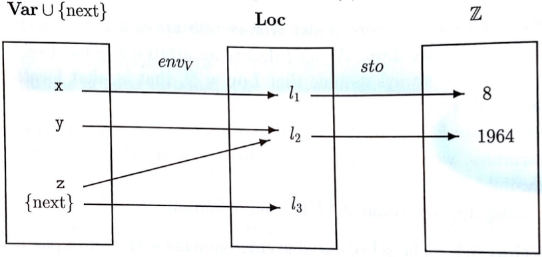
\includegraphics{resources/Images/stoloc.png}
    \caption{Environment-store model illustration \cite{stoloc}}
    \label{fig:Env}
\end{figure}

The following tables are the big step semantics of \lang{}.

\begin{table}[H]
\begin{adjustbox}{center}
\begin{tabular}{|c|c|}
\hline
\vspace {0.1pt} & \\
Num             &   \hbox{\Large \(env_V\, \vdash \langle n\: ,\ sto \rangle \rightarrow_a (v\: ,\ sto') \)\normalsize\(\quad \textbf{if}\ N\llbracket n \rrbracket = v  \)}  \vspace{0.1pt} \\ \hline 
\vspace {0.1pt} & \\  
Var             & \hbox{\Large \(env_V\, \vdash \langle x\: ,\ sto \rangle \rightarrow_a (v\: ,\ sto')\)\normalsize\( \quad \textbf{if} \: \begin{aligned}  env_V\ x=l \\ sto\ l = v \end{aligned} \)} \vspace {0.1pt} \\ \hline
\end{tabular}
\end{adjustbox}
    \caption{Num and var}
    \label{fig:declExp}
\end{table}

\begin{table}[H]
\begin{adjustbox}{center}
\begin{tabular}{|c|c|}
\hline
\vspace {0.1pt} & \\
Var-Decl      & \pbox{20cm}{ \huge \(\frac{env_C\, \vdash \langle D_V\: ,\ env_V']\rangle \rightarrow_{DV}\: (env'_V)}{env_C\, \vdash \langle dcl\ var\ x\ D_V\: ,\ env_V \rangle \rightarrow_{DV}\: env'_V} \)  \\ \\ \\ \normalsize \(  \textbf{where}\quad \: \begin{aligned} l=env_V\ next \\ env_V' = env_V[x \mapsto l][next \mapsto new\ l] \end{aligned} \)} \vspace {0.1pt} \\ \hline
\vspace {0.1pt} & \\
Empty-Var       & \hbox{\Large \(\langle \varepsilon\: ,\ env_V \rangle \rightarrow_{DV} env_V\)} \vspace {0.1pt} \\ \hline

\end{tabular}
\end{adjustbox}
    \caption{Declaration expressions}
    \label{fig:DeclarationExp}
\end{table}

\begin{table}[H]
\begin{adjustbox}{center}
\begin{tabular}{|c|c|}

\hline
\vspace {0.1pt} & \\
Relations 1     &   \pbox{20cm}{\Large \(env\, \vdash \langle a_1\: ,\ sto \rangle \rightarrow_a\: (v_1\: ,\ sto'')\) \\ \huge \(\frac{env\, \vdash \langle a_2\: ,\ sto'' \rangle \rightarrow_a\: (v_2\: ,\ sto')}{env\, \vdash \langle a_1\ op\ a_2\: ,\ sto' \rangle \rightarrow_b\: (\textit{tt}\: ,\ sto')}\)\normalsize\( \quad \begin{aligned} \textbf{if} \ v_1\ op\ v_2 \\ \textbf{where}\  op \in \{=, !=, >, <, >=, <= \}\end{aligned} \)}  \vspace{0.1pt} \\ \hline 
\vspace {0.1pt} & \\  
Relations 2     & \pbox{20cm}{\Large \(env\, \vdash \langle a_1\: ,\ sto \rangle \rightarrow_a\: (v_1\: ,\ sto'')\) \\ \huge \(\frac{env\, \vdash \langle a_2\: ,\ sto'' \rangle \rightarrow_a\: (v_2\: ,\ sto')}{env\, \vdash \langle a_1\ op\ a_2\: ,\ sto \rangle \rightarrow_b\: (\textit{ff}\: ,\ sto')}\)\normalsize\( \quad \begin{aligned} \textbf{if} \ \neg(v_1\ op\ v_2) \\ \textbf{where}\ op \in \{=, !=, >, <, >=, <= \}\end{aligned} \)} \vspace {0.1pt} \\ \hline
\vspace {0.1pt} & \\
Not 1           & \hbox{\huge\(\frac{env\, \vdash \langle b\: ,\ sto \rangle \rightarrow_b\: (\textit{tt}\: ,\ sto')}{env\, \vdash \langle not\ b\: ,\ sto \rangle \rightarrow_b\: (\textit{ff}\: ,\ sto')}\)} \vspace {0.1pt}\\ \hline
\vspace {0.1pt} & \\  
Not 2           & \hbox{\huge\(\frac{env\, \vdash \langle b\: ,\ sto \rangle \rightarrow_b\: (\textit{ff}\: ,\ sto')}{env\, \vdash \langle not\ b\: ,\ sto \rangle \rightarrow_b\: (\textit{tt}\: ,\ sto')}\) } \vspace {0.1pt}\\ \hline
\end{tabular}
\end{adjustbox}
    \caption{Boolean expressions}
    \label{fig:BooleanExp}
\end{table}

\begin{table}[H]
    \centering
    \begin{tabular}{|c|c|}

    \hline
    \vspace {0.1pt} & \\
And 1     & \pbox{20cm}{\Large \(env_V\, \vdash \langle b_1\: ,\ sto \rangle \rightarrow_b (\textit{tt}\: ,\ sto'')\) \\ \huge\(\frac{env_V\, \vdash \langle b_2\: ,\ sto'' \rangle \rightarrow_b\: (v\: ,\ sto')}{env_V\, \vdash \langle b_1\ and\ b_2\: ,\ sto \rangle \rightarrow_b (v\: ,\ sto')}\) } \vspace{0.1pt} \\ \hline 
    \vspace {0.1pt} & \\
And 2     & \hbox{\huge\(\frac{env_V\, \vdash \langle b_1\: ,\ sto \rangle \rightarrow_b (\textit{ff}\: ,\ sto')}{env_V\, \vdash \langle b_1\ and\ b_2\: ,\ sto \rangle \rightarrow_b (\textit{ff}\: ,\ sto')}\)} \vspace{0.1pt} \\ \hline 
    \vspace {0.1pt} & \\
Or 1     & \hbox{\huge\(\frac{env_V\, \vdash \langle b_1\: ,\ sto \rangle \rightarrow_b (\textit{tt}\: ,\ sto')}{env_V\, \vdash \langle b_1\ or\ b_2\: ,\ sto \rangle \rightarrow_b (\textit{tt}\: ,\ sto')}\)} \vspace{0.1pt} \\ \hline 
    \vspace {0.1pt} & \\
Or 2     & \pbox{20cm}{\Large \(env_V\, \vdash \langle b_1\: ,\ sto \rangle \rightarrow_b (\textit{ff}\: ,\ sto'')\) \\ \huge\(\frac{env_V\, \vdash \langle b_2\: ,\ sto'' \rangle \rightarrow_b\: (v\: ,\ sto')}{env_V\, \vdash \langle b_1\ or\ b_2\: ,\ sto \rangle \rightarrow_b\: (v\: ,\ sto')}\) }  \vspace{0.1pt} \\ \hline 
    \end{tabular}
    \caption{Gate expressions}
    \label{fig:GatesExp}
\end{table}

\begin{table}[H]
\begin{adjustbox}{center}
    \begin{tabular}{|c|c|}

    \hline
    \vspace {0.1pt} & \\
Parentheses & \hbox{\huge\(\frac{env_V\, \vdash \langle a\: ,\ sto \rangle \rightarrow_a\: (v\: ,\ sto')}{env_V\, \vdash \langle (a)\: ,\ sto \rangle \rightarrow_a\: (v\: ,\ sto')}\)} \vspace{0.1pt} \\ \hline 
    \vspace {0.1pt} & \\
    \(\begin{aligned}
\textrm{Addition} \\ \textrm{Subtraction} \\ \textrm{Multiplication}\end{aligned}\)  &   \pbox{20cm}{\Large\(env_V\, \vdash \langle a_1\: ,\ sto \rangle \rightarrow_a \: (v_1\: ,\ sto'')\) \\ \huge \(\frac{env_V\, \vdash \langle a_2\: ,\ sto'' \rangle \rightarrow_a\: (v_2\: ,\ sto')}{env_V\, \vdash \langle a_1\ op\ a_2\: ,\ sto \rangle \rightarrow_a \: (v\: ,\ sto')}\)\normalsize\( \quad \textbf{where} \quad op \in \{+,-,\cdot \} \)} \vspace{0.1pt} \\ \hline 
    \vspace {0.1pt} & \\
\(\begin{aligned}\textrm{Division} \\ \textrm{Modulo}\end{aligned}\)   & \pbox{20 cm}{\Large \(env_V\, \vdash \langle a_1\: ,\ sto \rangle \rightarrow_a (v_1\: ,\ sto'')\) \\ \huge \(\frac{env_V\, \vdash \langle a_2\: ,\ sto'' \rangle \rightarrow_a\: (v_2\: ,\ sto')}{env_V\, \vdash \langle a_1\ op\ a_2\: ,\ sto \rangle \rightarrow_a\: (v\: ,\ sto')}\)\normalsize\( \quad \textbf{where} \ \begin{aligned} op \in \{/,mod\} \\ v_2 \neq 0 \end{aligned} \)} \vspace{0.1pt} \\ \hline 
    \vspace {0.1pt} & \\
Unary   & \hbox{\huge\(\frac{env_V\, \vdash \langle a\: ,\ sto \rangle \rightarrow_a\: (v\: ,\ sto')}{env_V\, \vdash \langle -a\: ,\ sto \rangle \rightarrow_a\: (v\: ,\ sto')}\)\normalsize\( \quad \textbf{where} \quad v = -v\)} \vspace{0.1pt} \\ \hline 
    \end{tabular}
\end{adjustbox}
\caption{Arithmetic expressions}
\label{fig:ArithmeticExp}
\end{table}

\begin{table}[H]
\begin{adjustbox}{center}
\begin{tabular}{|c|c|}
\hline
\vspace {0.1pt} & \\
  if 1 &  \pbox{20cm}{\huge\(\frac{env_{VMC}\, \vdash \langle B_1\: ,\ sto'' \rangle \rightarrow (sto'\: ,\ Heap')}{ env_{VMC}\, \vdash \langle if\ b\ then\ B_1\ else\ B_2\ end\: ,\ sto\ \rangle \rightarrow sto'}\) \\ \normalsize\(\textbf{if} \quad env_V\, \vdash \langle b\: ,\ sto \rangle \rightarrow_b (\textit{tt}\: ,\ sto'')\)} \vspace{0.1pt} \\ \hline 
    \vspace {0.1pt} & \\
 if 2 &   \pbox{20cm}{\huge\(\frac{env_{VMC}\, \vdash \langle B_2\: ,\ sto'' \rangle \rightarrow (sto', Heap')}{ env_{VMC}\, \vdash \langle if\ b\ then\ B_1\ else\ B_2\ end\: ,\ sto\ \rangle \rightarrow sto'}\) \\ \normalsize\(\textbf{if} \quad env_V\, \vdash  \langle b\: ,\ sto \rangle \rightarrow_b (\textit{ff}\: ,\ sto'')\)} \vspace{0.1pt} \\ \hline 
    \vspace {0.1pt} & \\
  while 1 &  \pbox{20cm}{\Large \(env_{VMC}\, \vdash \langle B,\: sto'' \rangle \rightarrow (sto'''\: ,\ Heap'')\)\\
  \huge \(\frac{env_{VMC}\, \vdash \langle while\ b\ do\ B\ end\: ,\ sto'''\: ,\ Heap \rangle \rightarrow (sto'\: ,\ Heap)}{env_{VMC}\, \vdash \langle while\ b\ do\ B\ end\: ,\ sto \rangle \rightarrow (sto'\: ,\ Heap')} \) \\ \normalsize\(\textbf{if} \quad env_V\, \vdash \langle b\: ,\ sto \rangle \rightarrow_b (\textit{tt}\: ,\ sto'')\)} \vspace{0.1pt} \\ \hline 
\vspace {0.1pt} & \\
  while 2 &  \pbox{20cm}{\Large\(env_{VMC}\, \vdash \langle while\ b\ do\ B\ end\: ,\ sto\: ,\ Heap \rangle \rightarrow (sto'\: ,\ Heap)\) \\ \normalsize\(\textbf{if} \quad env_V\: ,\ env_C \, \vdash  \langle b\: ,\ sto \rangle \rightarrow_b (\textit{ff}\: ,\ sto')\)} \vspace{0.1pt} \\ \hline 
\vspace {0.1pt} & \\
  \(\begin{aligned} \textrm{for} \\ \textrm{upto 1} \end{aligned}\) &  \pbox{20cm}{\Large\(env_{VMC}\, \vdash \langle for\ x\ upto\ e\ do\ B\ end\: ,\ sto'\: ,\ Heap \rangle \rightarrow (sto'\: ,\ Heap) \) \\  \\ \normalsize \(\textbf{where}\ \begin{aligned} env_V\: ,\ env_C\, \vdash \langle x\: ,\ sto \rangle \rightarrow (v\: ,\ sto) \\ env_V\: ,\ env_C\, \vdash \langle e\: ,\ sto \rangle \rightarrow (v'\: ,\ sto')\\ v > v' \end{aligned}\) } \vspace{0.1pt} \\ \hline 
  \vspace {0.1pt} & \\
  \(\begin{aligned} \textrm{for} \\ \textrm{upto 2} \end{aligned}\) &  \pbox{20cm}{\Large \(env_{VMC}\, \vdash \langle B\: ,\ sto'' \rangle \rightarrow (sto'''\: ,\ Heap'')\) \\ \huge \(\frac{env_{VMC}\, \vdash \langle for\ x\ upto\ n\ do\ B\ end\: ,\ sto'''[l \mapsto v+1]\: ,\ Heap'' \rangle \rightarrow (sto'\: ,\ Heap')}{env_{VMC}\, \vdash \langle for\ x\ upto\ e\ do\ B\ end\: ,\ sto \rangle \rightarrow (sto'\: ,\ Heap')}\) \\ \\ \\ \normalsize\(\quad \textbf{where} \begin{aligned} env_V\: ,\ env_C\, \vdash \langle x\: ,\ sto \rangle \rightarrow (v\: ,\ sto) \\ env_V\: ,\ env_C\, \vdash \langle e\: ,\ sto \rangle \rightarrow (v'\: ,\ sto'') \\ n = N^{-1}[v'] \\ l=env_v\ x \\ v \leq v'  \end{aligned}\)} \vspace {0.1pt} \\ \hline
\end{tabular}
\end{adjustbox}
\caption{Control blocks}
    \label{fig:ControlBlock}
\end{table}

The 'for downto 1-2' are not displayed, as these are identical to 'for upto 1-2' with a few adjustments. The 'upto' operation is replaced with 'downto'. \(v\) has to, in 'downto 1', be less than \(v'\) instead of greater. In 'downto 2', \(v\) has to be greater than or equals \(v'\) instead of less than or equals. Lastly, \(l\) has to, in 'downto 2', map to \(v-1\) instead of \(v+1\). \\


For the sake of readability, \(env_V\: ,\ env_M\) are written as \(env_{VM}\) and \(env_V\: ,\ env_M\: ,\ env_C\) are written as \(env_{VMC}\). The for loop is split into four parts. Two for counting up and two for counting down, although the ones for counting down are, as mentioned above, not displayed. The 'for upto 1' is executed when the value of x is greater than the value of e. This is seen in the side conditions, where the value \(v\) of x, placed in \(sto\), has to be greater than the value \(v'\) of e, placed in \(sto''\), for it to be executed. Since the loop does not run, the storage does not change. 

The 'for upto 2' is executed when the value of x is smaller than the value of e. This is therefore the part that runs the statement in the for loop every time the before-mentioned side condition is true. The first precondition indicates that S is placed in sto''. The reason why this is not just \(sto\) is the fact that it is not necessarily the starting state. This state is executed and placed in \(sto'''\). The second precondition turns the value of e into a numeral with n, which is obtained as \(n = N^{-1}\llbracket v' \rrbracket \), and counts up the location defined by \(l = env_V\ x\) before placing it in \(sto'\).



%in the for upto 2 there is a bit more since this runs more then ones,  the first line \(\langle S,\ Sto''\rangle \rightarrow sto'''\) this say that it will run S, then in the next we count op the \(v\) of location l to \(v + 1\) and then ends, this can run if \(v \leq v'\) where x is stored in \(v\) and e is stored in the \(v'\), it also chance the value \(v'\) to the numerul n \(n=N^{-1}\llbracket v'\rrbracket\) and the location l is equal to the variable x in this enverememt.
\section{Scope Rules of \lang{}}
In \lang{}, the scope rules are fully static scope rules, as it has static scope rules for variables and static scope rules for functions. This means that both the variables and functions are bound when they are declared. 
\begin{comment}
\begin{table}[H]
    \begin{adjustbox}{center}
        \begin{tabular}{|c|c|}

\hline
\vspace {0.1pt}  &\\
PROC          &   \hbox{\huge \(\frac{env_V \vdash \langle D_P,\  env_P [p \mapsto (S,\  env_P)] \rangle \rightarrow_{DP} env'_P}{env_V \vdash \langle proc\ p\ is\ S;\ D_P,\ env_P \rangle \rightarrow_{DP} env'_P}\) } \vspace{0.1pt} \\ \hline 
\vspace {0.1pt} & \\  
PROC-EMPTY    & \hbox{\huge \(env_V \vdash \langle \varepsilon, env_P \rangle \rightarrow_{DP} env_P \)} \vspace {0.1pt} \\ \hline
\vspace {0.1pt} & \\ 
CALL-STAT-DYN & \hbox{\huge \(\frac{e'v[next \rightarrow e], e_p \vdash \langle S, \  st\rangle \rightarrow St'}{e_v , e_p \vdash \langle Call \  p, St \rangle \rightarrow St'} \ where \begin{aligned} e_p (p) = \langle S, e'_v \\ e = e_v (next) \end{aligned}\) } \vspace{0.1pt}  \\ \hline

        \end{tabular}
    \end{adjustbox}
    
    \caption{Caption}
    \label{fig:TrannyRulesProc}
\end{table}
\end{comment}
On the table \ref{fig:Func} the transition rules for function declarations are shown in the first two rows and the transition rule for function calls in the last row.


\begin{table}[H]
    \begin{adjustbox}{center}
        \begin{tabular}{|c|c|}
        \hline
\vspace {0.1pt} &\\
FUNC-Dcl        &   \hbox{\huge \(\frac{env_V\, \vdash \langle D_M\: ,\  env_M [f \mapsto (B\: ,\  env_M)] \rangle \rightarrow_{DM}\: env'_M}{env_V \vdash \langle func\ f(e_1\: ,\ ...\: ,\ e_n)\ begin\ B\ end\ D_M \ env_M \rangle \rightarrow_{DM}\: env'_M}\) } \vspace{0.1pt} \\ \hline 
\vspace {0.1pt} & \\  

Empty-FUNC-Dcl        &   \hbox{\Large \(env_V\, \vdash \langle \varepsilon\: ,\ env_F \rangle \rightarrow_{DF}\: env_F\) } \vspace{0.1pt} \\ \hline 
\vspace {0.1pt} & \\  

Func-Call  & \pbox{20cm}{\large \(env'_V\: ,\ env_M\, \vdash \langle B\: ,\ sto'' \rangle \rightarrow sto'\) \\ \huge \(\frac{env_M\, \vdash \langle PList\: ,\ sto\: ,\ env_V \rangle \rightarrow_{PList}(sto''\: ,\ env'_V)}{env\, \vdash \langle f(Plist)\: ,\ sto)\rightarrow sto'}\) \normalsize \\ \\ \(\textbf{Where} \quad PList \in \{x_1\: ,\ ...\: ,\ x_n\} \) } \vspace{0.1pt}  \\ \hline

        \end{tabular}
    \end{adjustbox}
    
    \caption{Functions call and declaration}
    \label{fig:Func}
\end{table}


\begin{table}[H]
    \begin{adjustbox}{center}
        \begin{tabular}{|c|c|}
        \hline
\vspace {0.1pt} &\\
EMPTY & \hbox{\Large \(env_V\: ,\ env_C\, \vdash \langle \varepsilon\: ,\ \varepsilon\: ,\ env_V\: ,\ sto \rangle \rightarrow (env_V\: ,\ sto)\)}\vspace{0.1pt} \\ \hline 
\vspace {0.1pt} & \\
ByRef & \pbox{20cm}{\huge \(\frac{\langle PList\: ,\ AList\: ,\ env''_V\: ,\ sto \rangle \rightarrow (env'_V\: ,\ sto')}{env_C\: ,\ env_C\, \vdash \langle y\ PList\: ,\ x\ AList\: ,\ env_V\: ,\ sto \rangle \rightarrow (env'_V\: ,\ sto')}\) \normalsize \\ \\ \(\textbf{Where} \begin{aligned} env_V[x\, \mapsto e] = env''_V \\ env_V(y) = e \end{aligned}\)} \vspace{0.1pt} \\ \hline 
\vspace {0.1pt} & \\
ByVal & \pbox{20cm}{\huge \(\frac{\langle PList\: ,\ AList\: ,\ env''_V\: ,\ sto'' \rangle \rightarrow (env'_V\: ,\ sto')}{env_V\: ,\ env_C\, \vdash \langle e\ PList\: ,\ x\ AList\: ,\ env_V\: ,\ sto \rangle \rightarrow (env'_V\: ,\ sto')}\) \normalsize \\ \\ \(\textbf{Where} \begin{aligned} env_V\, \vdash \langle e\: ,\ sto \rangle \rightarrow_e\: (v\: ,\ sto'') \\ env''_V = env_V[x\, \mapsto l][next\, \mapsto new\ l] \\ l = new(env_V\ next) \\ sto'' = sto[l \rightarrow v] \end{aligned} \)} \vspace{0.1pt} \\ \hline 
       
        \end{tabular}
    \end{adjustbox}
    
    \caption{PList Semantics}
    \label{fig:Plist}
\end{table}

In \lang{}, functions and a class constructor can take a set of defined parameters. These can both be by value and by reference. These is defined by PList. Their big-step semantics are defined in table \ref{fig:Plist}. The first rule, EMPTY, is called when the current parameter does not exist. Here, empty is returned. The Plist byRef starts with the \(env''_V\), as it is recursive, so there are possible information from earlier that needs to be taken into consideration. It saves the new information in the \(env'_V\) and \(sto'\), where the location of y is stored and passed on. The ByVal takes the value from the e that is in the \(env_V\) and stores the value from it in \(sto''\). Afterwards, it makes a new variable x that has a new location assigned to it, where it stores the value v.


\begin{table}[H]
    \begin{adjustbox}{center}
        \begin{tabular}{|c|c|}
        \hline
\vspace {0.1pt} &\\
Class-Dcl        &   \pbox{20cm}{\huge \(\frac{env_{VM}\, \vdash \langle P\: ,\ env''_C \rangle \rightarrow_{DC}\: env'_C}{env_{VM}\, \vdash \langle class\ c\ is\ c'\ begin\ D_V\ D_M\ end\ P\: ,\ env_C \rangle \rightarrow_{DC}\: env_C}\) \\ \\ \\ \normalsize \(\textbf{Where} \begin{aligned} env_C(c') = (env''_V\: ,\ env''_M) \\ env_C\, \vdash \langle D_V\: ,\ env''_V \rangle \rightarrow_{DV}\: env'_V \\ env'_V\, \vdash \langle D_M\: ,\ env''_M \rangle \rightarrow_{DM}\: env_M' \\ env''_C = env_C [c\, \mapsto(env_V'\: ,\ env_M')] \end{aligned} \)} \vspace{0.1pt} \\ \hline 
\vspace {0.1pt} & \\  

Class-instantiation &   \pbox{20cm}{\Large \(env''_V\: ,\ env_C\, \vdash \langle B\: ,\ sto''\: ,\ Heap \rangle \rightarrow (sto'\: ,\ Heap'')\) \\ \huge \(\frac{env_V\, ,\ env_C\, \vdash \langle PList\: ,\ AList\: ,\ env'_V\: ,\ sto \rangle \rightarrow (env''_V\: ,\ sto'')}{env_V\: ,\ env_C\, \vdash \langle set\ y\ to\ new\ c(PList)\: ,\ sto\: ,\ Heap \rangle \rightarrow (sto'\: ,\ Heap')}\) \\ \\ \\ \normalsize \(\textbf{Where} \begin{aligned} Heap' = Heap''[y\, \mapsto (env''_V\: ,\ sto\: ,\ Heap'')] \\ env_C(c) = (env'_V\: ,\ env_M) \\ env_M(OnConstruct) = (B\: ,\ AList\: ,\ env'_V) \end{aligned}\)} \vspace{0.1pt} \\ \hline
%Class-instantiation &   \pbox{20cm}{\Large \(env_C\, \vdash \langle D_V\: ,\ env_V\: ,\ sto \rangle \rightarrow (env''_V\: ,\ sto'')\) \\ \(env''_V\: ,\ env^1_C\, \vdash \langle D_M\: ,\ env^1_M \rangle \rightarrow env''_M\)\huge \\ \(\frac{env''_C\, \vdash \langle D_C\: ,\ envC[c\, \mapsto l]\: ,\ sto'''' \rangle \rightarrow \langle env'_V\: ,\ sto' \rangle}{env_C\, \vdash \langle set\ y\ to\ new\ c(Plist) \: ,\ env_C\: ,\ sto \rangle \rightarrow (env'_C\: ,\ sto')}\) \\ \\ \\ \normalsize \( \textbf{Where}\begin{aligned} env_C\ c = (B\: ,\ env_V\: ,\ env_M\: ,\ env_C) \\ l = sto'''\ next \\ sto'''' = sto'''[l \mapsto env''_V\: ,\ env''_M\: ,\ env''_C][next \mapsto new\ l] \end{aligned}\)} \vspace{0.1pt} \\ \hline 


    \end{tabular}
    \end{adjustbox}
    
    \caption{Caption}
    \label{fig:TrakhjnnyRulesProc}
\end{table}
    

When \lang{} returns a primitive value, the value is placed in a specific location, where it is retrievable after the function call. This location is called \textbf{retVar}, which is defined as: \(\textbf{retVar} = \textbf{Loc}\).

\begin{table}[H]
    \begin{adjustbox}{center}
        \begin{tabular}{|c|c|c|}
        \hline
\vspace {0.1pt} &\\
Assignment      &   \pbox{20cm}{\Large \(env_{VM}\, \vdash \langle set\ x\ to\ e\: ,\ sto \rangle \rightarrow sto'[l \mapsto v] \quad\)\\ \\ \( \textbf{where}\ \begin{aligned} env_{VM}\, \vdash \langle e\: ,\ sto \rangle \rightarrow \: (v\: ,\ sto') \\ l = env_V\ x \end{aligned} \) } \vspace{0.1pt} \\ \hline 
\vspace {0.1pt} & \\

Block       &   \pbox{20cm}{\Large \( \langle D_V\: ,\ env_V \rangle \rightarrow_{DV} env'_V \) \\ \huge \(\frac{env'_V\: ,\ env_M\, \vdash \langle S\: ,\ sto \rangle \rightarrow sto'}{env_{VM}\, \vdash \langle \{D_V\ S \}\: ,\ sto \rangle \rightarrow sto'} \) } \vspace{0.1pt} \\ \hline 
\vspace {0.1pt} & \\
Skip       &   \pbox{20cm}{\Large \( env_{VM}\, \vdash \langle skip\: ,\ sto \rangle \rightarrow sto \) } \vspace{0.1pt} \\ \hline 
\vspace {0.1pt} & \\

Composite       &   \pbox{20cm}{\Large \(env_{VM}\, \vdash \langle S_1\: ,\ sto \rangle \rightarrow sto''\) \\ \huge \(\frac{env_{VM}\, \vdash \langle S_2\: ,\ sto'' \rangle \rightarrow sto'}{env_{VM}\, \vdash \langle S_1\ S_2\: ,\ sto \rangle \rightarrow sto'}\) } \vspace{0.1pt} \\ \hline 
\vspace {0.1pt} & \\

Return Primitive          & \hbox{\huge \(\frac{env_{VM}\, \vdash \langle x\: ,\ retVar\: ,\ sto \rangle \rightarrow\: retVar'\: ,\ sto}{env_V\, \vdash \langle return\: x,\ env_V\: ,\ sto \rangle \rightarrow\: retVar'\: ,\ env_V\ sto}\) } \vspace{0.1pt}  \\ \hline
\vspace {0.1pt} & \\

Return Reference      & \hbox{\huge \(\frac{env_{VM}\, \vdash \langle y\: ,\ sto \rangle \rightarrow\: sto'}{env_V\, \vdash \langle return\: y,\ env_V\: ,\ sto \rangle \rightarrow\:  env_V'\ sto'}\) } \vspace{0.1pt}  \\ \hline

        \end{tabular}
    \end{adjustbox}
    \caption{Caption}
    \label{fig:hgf}
\end{table}

\begin{table}[H]
    \begin{adjustbox}{center}
        \begin{tabular}{|c|c|c|}
        \hline
\vspace {0.1pt} &\\
Program1      &   \pbox{20cm}{\Large \(env_V\, \vdash \langle D_V\: ,\ env_V\: ,\ sto \rangle \rightarrow (env''_V\: ,\ sto') \)\huge \\ \(\frac{env''_{VMC}\, \vdash \langle M_C\: ,\ env_C \rangle \rightarrow env'_C }{env_{VMC}\, \vdash \langle D_V\: ,\ M_C\: ,\ sto \rangle \rightarrow sto'} \) } \vspace{0.1pt} \\ \hline 
\vspace {0.1pt} & \\
Program2     &   \pbox{20cm}{\huge  \(\frac{env_{VMC}\, \vdash \langle D_C\: ,\ env_C \rangle \rightarrow env'_C }{env_{VMC}\, \vdash \langle D_C P\: ,\ sto \rangle \rightarrow sto'} \) } \vspace{0.1pt} \\ \hline 

        \end{tabular}
    \end{adjustbox}
    
    \caption{Program}
    \label{fig:progstuff}
\end{table}



This concludes the semantics chapter, where the abstract syntax was presented, the operational semantics were specified and where it was explained how the type rules and scope rules of \lang{} work. 
Now that all the semantics of \lang{} have been formally specified, a description of the implementation of \lang{} will follow.
\chapter{Implementation}
This chapter explains the different phases of the \lang{} compiler, and how they were implemented for the \lang{} compiler. The \lang{} compiler has several distinct phases, as seen on \ref{fig:compphase}. 


\begin{figure}[H]
    \centering
    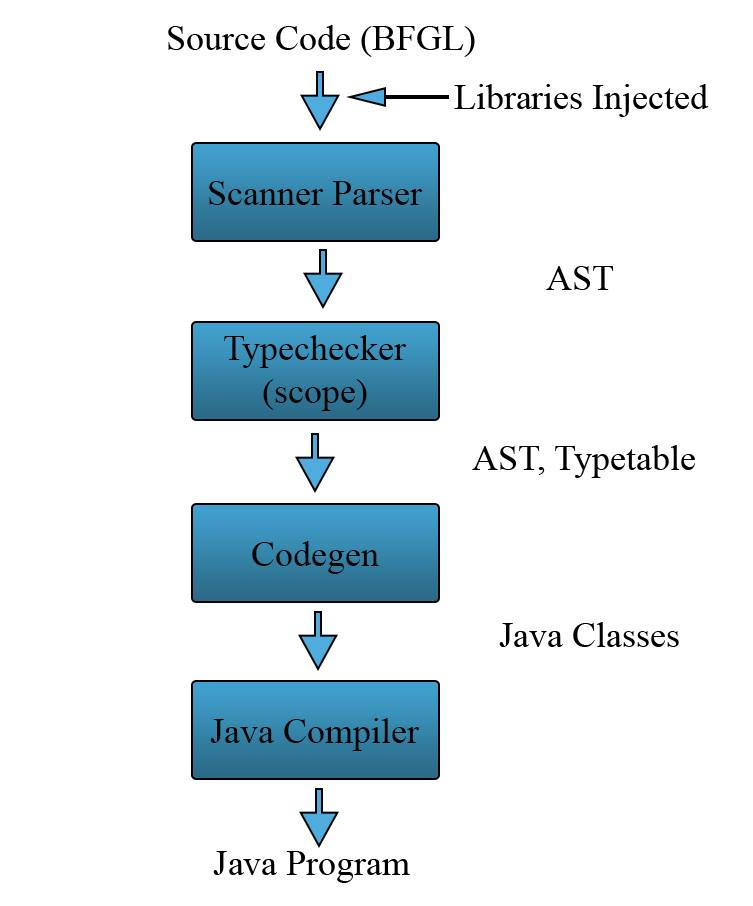
\includegraphics[scale=0.5]{resources/Images/compiler-phase.jpeg}
    \caption{A generalized figure of the phases of the \lang{} compiler.}
    \label{fig:compphase}
\end{figure}

These phases are:

\begin{itemize}
    \item Library injection
    \item Scanner and Parser
    \item Type checker
    \item Code generator
    \item Java Compiler
\end{itemize}

The \lang{} compiler, as a whole, takes a file with code written in \lang{} as input and outputs an executable Java program.

The first thing that happens when a user wants to compile a \lang{} file in the \lang{} compiler, is that the \lang{} libraries are injected into the user's file. This is done to include the libraries in the AST, so that they are present when the type checker is run.

After the libraries are added to the source file, the file is run through the scanner and parser, which is generated by SableCC. This phase returns an AST of the program, which is used throughout the rest of the compiler.

The next phase, the type checker, performs a tree walk of the AST. During the walk, the type checker adds each node to a hash table with a reference to the node and the type of the node, adds all variables, methods and classes to a symbol table, validates the types of a node's child nodes and checks if the different variables, methods and classes are within the scope. When the type checking phase is complete, it is known whether or not the \lang{} program is semantically correct. The type table is also returned for use in the code generation phase of the compiler.

When the source program is confirmed to be a valid program in \lang{}, the code generation phase is initiated. In this phase, a new tree walk is done over the AST and code is generated for each node. When this phase is completed, a number of java files have been generated, which is afterwards run trough the final phase of the compiler, namely the Java Compiler.

The following sections gives a more in-depth explanation of the different phases of the \lang{} compiler, but before that, the Depth First adapter, used for the different tree walks, is explained.

\section{SableCC's Depth first adapter}
SableCC provides a depth first adapter class, which is intended to be used in later phases of the compiler to traverse the AST for analysis and code-generation purposes. When implementing the analysis and codegen phases, the depth-first adapter class can simply be extended, which, in the end, saves development time and reduces the amount of errors that could be introduced when implementing the compiler. The adapter implements two functions for each Node type in the AST. These are an \textit{in} and \textit{out} function. The \textit{in} function is called each time the tree walker enters, i.e the first time it visits a node, and the \textit{out} function is called when the tree walker has visited the whole sub-tree rooted in that node, i.e when it exits a node. An example template of how these \textit{in} and \textit{out} functions could look for a "Prog" node, which is always the first node to be created in the AST, is shown below:
\begin{figure}[H]
    \centering
    
    \begin{lstlisting}[style=gglang]
    public void inAProg(AProg node){
        
        //Some code to be executed on node entry here
    
    }
    public void outAProg(Aprog node){
    
        //Some code to be executed on node exit here
        
    }
    
    \end{lstlisting}
    \caption{Example for how the in and out methods are used in the \lang{} compiler\label{fig:inout}}
\end{figure}
There is of course a lot of other nodes, which can be found in the AST grammar in appendix \ref{AST}.
The different kinds of actions, that are needed in the analysis and code generation phases, are hereafter implemented as extensions of the DepthFirstAdapter class. This approach is used through the rest of the compiler. 

\section{Scanner and Parser phase}

The scanner (also known as the lexer) and parser used for \lang{} has been generated using SableCC, with a modified version of the grammar shown in Section \ref{sec:OurSyntax}. The actual code used with SableCC can be found in \ref{FGramma}. By running code in \lang{} through the parser, an Abstract Syntax Tree (AST) is generated, which will then be used in the semantic analysis phase, and in the code-generation phase.
The grammar definition is split into two parts. The first part defines the syntax of \lang{} and aids the creation of a CST structure, and the second part defines an AST structure for input generated by the first phase of the compiler. The CST is used internally by the code generated by SableCC, and is never touched in the implementation of \lang{}. The AST, however, is the result the syntax analysis phase produces, and it is what is used further on in the following phases. 
The grammar for the AST and the CST are very similar. The main difference is that the AST grammar can be ambigious, whereas the CST grammar must be unambigous. Both grammars can be found in the appendix, AST grammar at appendix \ref{AST}, and the CST at the top of appendix \ref{FGramma}. They are both written in the style required by SableCC, although still close to the original grammar.
\subsection{Implementation of Syntax in \lang{}}
The implementation of \lang{}'s syntax is handled entirely by SableCC, as it generates both the lexer and the parser. There is no custom code in this part of the compiler. It is all generated by SableCC. The only "custom" code is an object instance which contains the AST after being produced by the lexer/parser. The code used for calling the parser and lexer is implemented as follows:
\begin{figure}[H]
    \centering
    
    \begin{lstlisting}[style=gglang]
        PushbackReader pushbackReader = new PushbackReader(new FileReader(addLibrary(file)));
        Parser parser = new Parser(new Lexer(pushbackReader));
        Start tree = parser.parse();
    \end{lstlisting}
    \caption{The code for calling the parser and lexer.\label{fig:parslex}}
\end{figure}
"PushbackReader" is the lexer, and "Parser" is the parser. "tree" is the object instance containing the AST after the parser is done. 
\section{Type checker phase}
\label{sec:semanticAnal}
Besides generating a parser, SableCC also generates a \textit{tree walking} class, which can traverse the AST. This is done using a modified version of the visitor pattern, implemented by SableCC. 

To implement the type and scoping rules, defined formally in chapter \ref{chap:semantics}, a new class has been created, called \textit{TypeChecker}. This class inherits from a class generated by SableCC, called \textit{DepthFirstAdapter}, as described in the introduction to this chapter.  The \textit{in} and \textit{out} functions, that is described for all Nodes, will be used to implement the type and scoping rules. 

\subsection{Symbol table and scope}
The symbol table is implemented as a stack of \textit{hash tables}, indexed by an id string, i.e. the id of the variable or function in question, and value of a reference to the node where it is declared. Each time a new scope is opened, a new \textit{hash table} is pushed to the stack, and when a scope is closed, the hash table on top of the stack is removed. This makes sure that the current scope is always on top of the stack, and that only the nodes in scope are located in memory. 


\begin{figure}[H]
\centering
\begin{lstlisting}[]

    private void openScope(Node node){
        TableFiller tf = new TableFiller(node);

        node.apply(tf);

        symStack.push(tf.symStack.pop());
        typeTable.putAll(tf.typeTable);
        ErrorList.addAll(tf.ErrorList);
    }
    
\end{lstlisting}
\caption{Code example: \textit{openScope}}
\label{fig:openscope}
\end{figure}

When a new scope is opened, the function shown on figure \ref{fig:openscope} is called. This function initiates a new instance of the \textit{TableFiller} class, which also inherits from the \textit{DepthFirstAdapter}. When the TableFiller object is applied to a node, as seen on line 5 of figure \ref{fig:openscope}, it initiates a tree walk over the subtree with that node as the root. During this tree walk, it fills its own symbol table, by adding to it each time it encounters a declaration node. This symbol table is then popped, and the result is added to the actual symbol table stack, as seen on line 7.

This pass is done to make it possible to call a function or class that has not yet been declared in the code.

The TableFiller class implements \textit{out} functions for all the declaration nodes and \textit{in} functions for some of them.

To add a symbol to the symbol table, a function called addSymbol is called. This function is seen on figure \ref{fig:addsymbol}. The \textit{addSymbol} function takes a name and a node as parameters. These are the values that are added to the symbol table.

\begin{figure}[H]
\centering
\begin{lstlisting}[]

    private void addSymbol(String name, Node node){
        if (!symStack.peek().containsKey(name)) {
            symStack.peek().put(name, node);
        }
        else
            ErrorList.add("ERROR: " + name + " is already defined in this scope " + symStack.peek().size());
    }
    
\end{lstlisting}
\caption{Code example: \textit{addSymbol}}
\label{fig:addsymbol}
\end{figure}

Before adding the symbol to the symbol table, the function first makes a check to see if the symbol is already in the current scope (the symbol can be in an outer scope, since \lang{} has symbol shadowing). If the symbol is not found in the current scope, it is added, as seen on line 4 of figure \ref{fig:addsymbol}. If it is already in the current scope, an error message is added to an ArrayList called \textit{ErrorList}, which is a list of all the errors found. This will be used later on for displaying error messages.

To implement the dot operator, i.e '\textit{object\textbf{.}attribute}', the scope analyser must traverse the declaration sub tree for the class to check that it implements the attribute in question. This is done by applying the \textit{TableFiller} on the root of the class declaration sub tree. If a there are more than one level or more than one 'dot' in a call made with the dot operator, a new scope is opened for each class in the call with the current scope being the right most class in the call.



\subsection{Type Checker}
To implement the type rules, a new \textit{hash table} is used. This table is indexed by a node reference and its value is a string containing the type of that node. The value is a string and not a enum type, since in \lang{} the user can implement their own types. 

When talking about type checking, the nodes of the AST can be divided into four different categories, namely;

\begin{itemize}
    \item Nodes with no type.\\
    \textit{i.e main- and event-nodes}
    
    \item Nodes with a type. \\
    \textit{i.e value- and type-nodes}
    
    \item Nodes with a type, that is dependent of its child nodes.\\
    \textit{i.e function declaration- and expression-nodes}
    
    \item Nodes with no type, but with child nodes of a certain type.\\
    \textit{i.e if- and loop-nodes}
\end{itemize}

These different nodes are handled in different ways in the implementation of the type checker.

The first category of nodes are not handled in the type checking phase, since the nodes themselves always will be type-correct, and the type correctness of the child nodes will be validated on their respective nodes.

The second categories of nodes must be added to the type table. This is done by calling the function \textit{addType}, as seen on figure \ref{fig:addtype}. The call is made in the \textit{out} function of a node. The \textit{addType} function simply adds the node to the \textit{typeTable}. It is necessary to call \textit{trim()}, which removes white space at the start and end of the string.


\begin{figure}[H]
\centering
\begin{lstlisting}[]
    private void addType(Node node, String type){
        typeTable.put(node, type.trim());
    }
    
\end{lstlisting}
\caption{Code example: \textit{addType}}
\label{fig:addtype}
\end{figure}

An example of an \textit{out} function, as explained in \ref{sec:semanticAnal}, for a node in the second category can be seen on figure \ref{fig:outAFuncCall}.

\begin{figure}[H]
\centering
\begin{lstlisting}[]
    public void outAFuncCall(AFuncCall node){
        addType(node, getType(node.getId().getText()));
    }
    
\end{lstlisting}
\caption{Code example: \textit{outAFuncCall}}
\label{fig:outAFuncCall}
\end{figure}

Figure \ref{fig:outAFuncCall} shows how a node is added to the type table. In this example, the type is found by calling \textit{getType}, which searches the type-table. Some nodes, such as the different \textit{type} nodes, simply adds the string of their type.

The third category of nodes are the nodes whose type is dependent on the type of their child nodes. These include, but are not limited to, expression nodes.

Firstly, the child nodes' type is checked to evaluate if they meet the specification made in \ref{sec:TypeRules}. An example can be seen in the \textit{out} function of the \textit{plus-expression} node, as seen on figure \ref{fig:outAPlusExpr}.


\begin{figure}[H]
\centering
\begin{lstlisting}[]
    public void outAPlusExpr(APlusExpr node){
        if(typeTable.get(node.getLeft()).equals(TEXT) || typeTable.get(node.getRight()).equals(TEXT)){
            addType(node, TEXT);
        }
        else if(typeTable.get(node.getLeft()).equals(NUM)){
            if(typeTable.get(node.getRight()).equals(NUM)){
                addType(node, NUM);
            }
            else{
                ErrorList.add("ERROR line " + lineAndPos.getLine(node) + " pos " + lineAndPos.getPos(node) + " : " + node.getRight().toString() + ", is not of type " + NUM + ".");
                addType(node, ERRORTYPE);
            }
        }
        else{
            ErrorList.add("ERROR line " + lineAndPos.getLine(node) + " pos " + lineAndPos.getPos(node) + " : " + node.getLeft().toString() + ", is not of type " + NUM + ".");
            addType(node, ERRORTYPE);
        }
    }
    
\end{lstlisting}
\caption{Code example: \textit{outAPlusExpr}}
\label{fig:outAPlusExpr}
\end{figure}

In this example, if either of the child nodes are of type \textit{text}, the type of the whole expression is \textit{text}. The same goes for \textit{num}. If both these cases are false, an error is added to the ErrorList and the node gets the type \textit{ERRORTYPE}. This is done to allow the compiler to continue and collect all the errors, instead of stopping at the first type error encountered.

The fourth and last category of nodes are the nodes that are dependent on the type of one or more of their child nodes, but do not have a type themselves.

\begin{figure}[H]
\centering
\begin{lstlisting}[]
    public void outAForupStmt(AForupStmt node){
        closeScope();

        if(!typeTable.get(node.getExpr()).equals(NUM)){
            ErrorList.add("ERROR line " + lineAndPos.getLine(node.getExpr()) + " pos " + lineAndPos.getPos(node.getExpr()) + " : " + node.getExpr().toString() + ", is not of type " + NUM + ".");
        }

        if(!getType(node.getId().getText()).equals(NUM)){
            ErrorList.add("ERROR line " + lineAndPos.getLine(node.getId()) + " pos " + lineAndPos.getPos(node.getId()) + " : " + node.getId().toString() + ", is not of type " + NUM + ".");
        }
    }
    
\end{lstlisting}
\caption{Code example: \textit{outAForupStmt}}
\label{fig:outAForupStmt}
\end{figure}

An example of such a node is the \textit{ForupStmt} node. The \textit{out} function for this can be seen on figure \ref{fig:outAForupStmt}. This function only needs to control the types of the child nodes and thus not add anything to the type table.

Due to the fact that a function's type is not declared on the function declaration in \lang{}, the return type of the function must be found by examining the return node of the function declaration. To achieve this, the function declaration sub tree is traversed by applying the TypeChecker to the function declaration node. The type is then set to the type of the return node's expression child node. 

\subsubsection{Inheritance}
To obtain the inherited type of an object, it is necessary to add a new table, namely a super table. Each entry in the table contains two strings; one for the object's own type and one for the super type.

\subsubsection{Error handling}
If an error is encountered during compilation, one of two things can happen. If the error originates from the lexer/parser part of the compiler, for example a syntactical error, it is shown on the GUI, and compilation will be terminated. If the error, on the other hand, is from the semantic/contextual analysis phase, for example a semantic error, it is added to a List called errorlist, and the whole list is shown once the compilation is done or has reached a point where it cannot continue.

This concludes the section about the type-checker itself. The following chapter is about code-generation, and how it was implemented for the \lang{} compiler. 

\section{Code Generation phase}
The last phase of the compiler is the code-generation phase. In this phase, code is generated for the target language, which, in the case of \lang{}, is Java. The code generation is done using the AST produced by the previous compiler phases, and using the Sable-CC tree-walking method similarly as done in the previous phases. The code that calls the JavaCodeGenerator class to begin code generation for java is implemented as seen on figure \ref{fig:startcodegen}.

\begin{figure}[H]
    \centering
    
    \begin{lstlisting}[style=gglang]
            new JavaCodeGenerator(typeChecker.typeTable, typeChecker.superTable, tree);
            AntExecutor AEx = new AntExecutor();
            AEx.executeAntTask("CompileBFGL.xml", "jar");
    \end{lstlisting}
    \caption{The code for calling the class responsible for starting code generation.\label{fig:startcodegen}}
\end{figure}
The last two lines are not directly responsible for generating java code, but they execute the rest of the build process. This includes moving library-files to the right positions, calling the java compiler to compile the generated java code to .class files, and finally creating an executable .jar file with the compiled game contained inside.

\subsection{Code Generation for Java}
To accommodate the different needs of an object-oriented language, six different visitors were created based on the depth-first adapter from Sable-CC.
This uses the \textit{in} and \textit{out} functions, just like the semantic analysis did in the last section, as shown on \ref{fig:inout}.


\subsubsection{JavaCodeGenerator}
An instance of this class is created at the beginning of the codegen phase. The first thing it does is to add in some of the libraries contained in the Libraries folder, which is implemented as seen on figure \ref{fig:librarycodegen}.
\begin{figure}[H]
    \centering
    \begin{lstlisting}[style=gglang]
        addLibrary("Scene", "Scene");

        node.apply(new TopVisitor(typeTable, superTable));

        addLibrary("Main", "Main");
        addLibrary("MathBFGL", "MathBFGL");
    \end{lstlisting}
    \caption{Libraries are added \label{fig:librarycodegen}}
\end{figure}
The "addLibrary" method looks in the libraries folder and tries to import a library file according to what parameters were given. "Scene" is added before "Main" and "MathBFGL", because it contains some variables that have to be available before the TopVisitor runs.
These libraries contain setup code, that makes the Slick library work with the game, written in java. After having input these basic files into the compilation target folder, it calls Topvisitor to begin the rest of the code-generation. The Slick library contains a set of APIs used in the generated code, such as input handling, rendering/drawing, and basic collision detection. The setup done by the libraries, imported with JavaCodeGenerator, abstracts away a lot of the general setup that has to be done when making a game, which helps to simplify the code-generation process, as the whole feature set of the Slick library does not have to be reimplemented. This also enhances the reliability of the language and the games produced by it since the APIs of Slick have been extensively tested.

\subsubsection{TopVisitor}
Topvisitor is the first actual visitor to be applied to the AST in the code-generation phase. As the name suggests, it visits the different topmost level of the AST, namely the entry point of the game, the different classes, and the main method of the BFGL input file. This main is different from the java main-file, as the content of this main is input into the Slick version of an initialising constructor for the game to set up whatever, the user might want to set up, before the game starts running. 
In order for the Java files to work and compile properly, without having to write a complex function to determine what namespaces might be needed, any new class just has all the possible namespaces, it could need, added in per default. The implementation of this method for importing namespaces is just a list of all the namespaces that is used with the \lang{} specification, see figure \ref{fig:javaimport}.

\begin{figure}[H]
    \centering
    \begin{lstlisting}[style=gglang]
    protected void AddNameSpaces() {
        emitnl("import java.lang.*;");
        emitnl("import java.util.*;");
        emitnl("import java.io.*;");
        emitnl("import java.text.*;");
        emitnl("import java.awt.*;");
        emitnl("import java.nio.*;");
        emitnl("import java.math.*;");
        emitnl("import org.newdawn.slick.*;");
    }
    
    \end{lstlisting}
    \caption{Java library import}\label{fig:javaimport}
\end{figure}

This is of course not very efficient, but efficiency is not the main goal of \lang{}, as long as the games runs at a reasonable FPS(frames per second).
TopVisitor also imports all the global variables declared in the \lang{} file, and puts them in a class called Global, to facilitate calling them wherever it might be needed. The implementation of this is a simple copy from one file to another. 
TopVisitor has "in"  methods for both "prog", the entrypoint of a game, main, the main class in the \lang{} file, and for class, which corresponds to all the classes defined in the \lang{} file. 
The class "in" node method contains logic for adding in a lot of static libraries used by the language - most of which are simple wrapper-classes that call corresponding Java or Slick methods. This is necessary to make the classes available at compile time. Otherwise, the \lang{} compiler would throw exceptions and the compilation would fail. An example from one of the wrapper classes that are used, can be found on figure \ref{fig:wrapperClass}.

\begin{figure}[H]
\centering
    \begin{lstlisting}[style=gglang]
    dcl func roundDown(num numToBeRounded) begin
        return 0
    end

    dcl func round(num numToBeRounded) begin
        return 0
    end

    dcl func sqrt(num numToSqr) begin
        return 0
    end

    dcl func pwr(num howMuchToPower) begin
        return 0
    end

    dcl func getRandomNum(num upperBound) begin
        return 0
    end
    \end{lstlisting}
    \caption{Example of wrapper class used for mathematical funtions}\label{fig:wrapperClass}
\end{figure}
These functions are never a target for code generation. They are simply in the compilation process to make the functions available during the semantic analysis phase, after which they are replaced by one of the static libraries.

\subsubsection{ClassBodyVisitor and FuncBodyVisitor}
The purpose of these two classes is to visit the bodies of functions and classes, and emit corresponding Java code. These are made in two distinct classes instead of one, as they are logically distinct. A function-body can contain any amount of statements, while a class-body can contain a wider range of things, which has to be printed differently. An example from ClassBodyVisitor, of how a list is handled, is seen on figure \ref{fig:inAListPdcl}.

\begin{figure}[H]
    \centering
    \begin{lstlisting}[style=gglang]
     public void inAListPdcl(AListPdcl node) {
        if (!node.visited) {
            node.visited = true;
            emitnl("ArrayList<" + "_" + node.getType().toString().trim() + "> " + "_" + node.getId().getText() + " = new ArrayList<>();");

        }
    }
    \end{lstlisting}
    \caption{Example from ClassBodyVisitor}\label{fig:inAListPdcl}
\end{figure}


\subsubsection{ExpressionVisitor}
ExpressionVisitor visits all the different expression nodes, and emits the corresponding operators.

\begin{figure}[H]
    \centering
    \begin{lstlisting}[style=gglang]
    public void inAMinusExpr(AMinusExpr node) {
        if (!node.visited) {
            node.getLeft().apply(this);
            emit(" - ");
            node.getRight().apply(this);
            node.visited = true;
        }


    }
    \end{lstlisting}
    \caption{Examples of how the ExpressionVisitor corresponds to the semantics of \lang{}}\label{fig:inAMinusExpr}
\end{figure}

As is seen in figure \ref{fig:inAMinusExpr} example, when evaluating a minus expression, the left node will be evaluated, after which the symbol "-" will be added. Lastly, the right node is evaluated. As this is translated to Java, which will evaluate this from left to right, it ensures that the expression is evaluated in the correct order. 

\subsubsection{For loops}
For loops in \lang{} are implemented differently than most languages. They use two distinct syntaxes for loops going from a high value to a low value, or vice versa. This is specified by writing either "for x upto y do" or "for x downto y do". This is analysed and turned into Java code as seen on figure \ref{fig:downtobfgl}.

\begin{figure}[H]
\centering
    \begin{lstlisting}[style=gglang]
    for x downto 0 do
        set y to y + 1
    end
    \end{lstlisting}
    \caption{\lang{} down to}\label{fig:downtobfgl}
\end{figure}
Is turned into the code seen on figure \ref{fig:downtojava} when compiled using the \lang{} compiler.
\begin{figure}[H]
\centering
    \begin{lstlisting}[style=gglang]
    float _exprvalx = 0f;
    for(_x = _x ; _x >= _exprvalx ; _x--){
        _y = _y + 1f;
    }
    \end{lstlisting}
    \caption{Java translation of down to}\label{fig:downtojava}
\end{figure}

A thing to note is that the value to be repeated down to is evaluated once, and then stored in a variable called \_exprvalx. This is done to make the loop behave in correspondence with the semantics for for loops, as specified in the Semantics chapter \ref{fig:ControlBlock}.

\subsubsection*{Order of evaluation}
Evaluation order in \lang{} follows normal, sequential evaluation order, as seen in the example in figure \ref{fig:ecaluationorder}.

\begin{figure}[H]
    \centering
    \begin{lstlisting}
    dcl num n to 0
    dcl num out
    dcl func f() begin
        set n to n + 1
        return 1
    end
    dcl func g() begin
        set n to n * 2
        return 1
    end

    dcl func result() begin
        set n to 0
        set out to f() + g()
        dcl Label l to new Label("" + n, 100, 100) // expected: 2
        set n to 0
        set out to g() + f()
        dcl Label l1 to new Label("" + n, 100, 120) // expected: 1
    end
    \end{lstlisting}
    \caption{The evaluation order of functions in \lang{}}\label{fig:ecaluationorder}
\end{figure}

When "out" is set to \textit{f + g}, \textit{f} will be evaluated first, and then \textit{g}. Other cases of this was tested and verified, as described in the \ref{Test} chapter.

\subsubsection{DisableVisitor}
This visitor disables nodes after they have been visited. This is used in the code generation for class calls to prevent the same classes being written to the compiler output multiple times. A class call is a normal "something.someclass.somemethod" call, but if it was visited as it normally would, it would print out the classes multiple times. This is prevented by DisableVisitor by setting a boolean named "visited" to true. 


\section{The GUI of the \lang{} compiler}
In order to help ease the use of the \lang{} compiler, a simple GUI was created using Java Swing\cite{swing}. The only features it implements is a way to target a text file for compilation, followed by a button to execute the compilation. After the compilation is done, it opens the folder with the finished game. It looks as seen on figure \ref{fig:GUI}.
\begin{figure}[H]
\centering
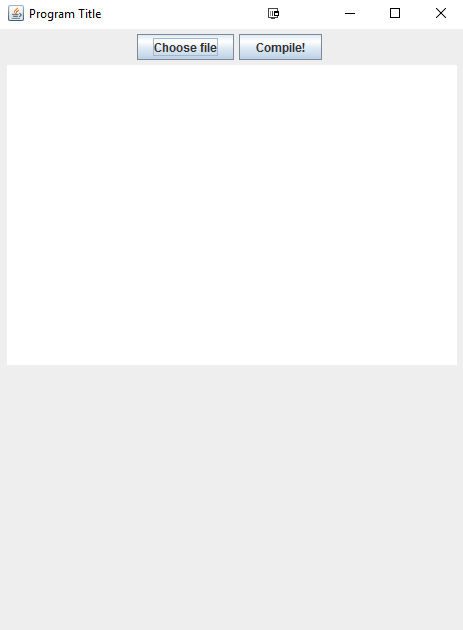
\includegraphics[scale=0.5]{resources/Images/Udklip.PNG}
\caption{The \lang{} GUI.)}\label{fig:GUI}
\end{figure}

The following section describes and presents the tests made on the \lang{} compiler.
\section{Test}\label{Test}
In this section, the testing, done on \lang{} to ensure the correctness of the output of the compiler, is described. 
\subsection{Compilation testing}
In order to keep track of whether or not something suddenly changed in the compiler implementation, both intentionally and unintentionally, a test was implemented to compare the current output of the compiler to a correct output of the compiler. This is based on a test file written in \lang{}, called \textit{BFGLtest.bfgl}. This makes sure that no unintentional changes happen, and that the compiler output stays the same. 
The comparison itself is done in several tests:
\begin{itemize}
    \item Test if the compilation \textit{out} folders are created.
    \item Test of the contents of the compilation \textit{out} folders, for example if they contain the right amount of files.
    \item MD5 comparison of all the files in the \textit{out} folders, to ensure that the files are all the exact same. 
\end{itemize}
The MD5 comparison uses a built-in class called "MessageDigest" from the java platform package "Security", which can produce MD5 hashes when given a binary representation of a data-object. The hashes of the objects are then compared. The implementation is as seen on figure \ref{fig:md5}.

\begin{figure}[H]
    \centering
    \begin{lstlisting}
        String hexCompiledFile;
        String hexTargetFile;
            if (targetFile != null && compiledFile != null){
                hexTargetFile = (new HexBinaryAdapter()).marshal(md5.digest(targetFile.getBytes()));
                hexCompiledFile =  (new HexBinaryAdapter()).marshal(md5.digest(compiledFile.getBytes()));

                if (hexTargetFile != null && hexCompiledFile != null){
                    assertTrue("Files are different! MD5 mismatch!" + i, hexTargetFile.equals(hexCompiledFile));
                }
            }
    \end{lstlisting}
    \caption{How the \lang{} compiler testing compares files using MD5.}\label{fig:md5}
\end{figure}

"assertTrue" is from the testing framework, and will report back whether or not the test failed. "MD5" is the MessageDigest object set to produce hashes.

The tests are build using Junit4, which is a testing framework that comes bundled with the IDE used in the development process(Intellij IDEA, \cite{intellij}). The use of Junit4 allows more time to be spent on the tests themselves, instead of spending a lot of time on the setup of the testing suite/program. It also allows to separate tests for different parts of the compiler into different classes, and then calling them all through a "Test Suite" that runs the tests. 
\todo{add intellij to bibtex breh}


\subsection{Blackbox tests}
This kind of test is not about programatically checking the code/compiler output for errors and unintended change. It is about running the compiler through extreme use-cases and other critical points to see if it still behaves accordingly, and visually verifying that this is the case. This was done throughout the implementation of the compiler, but in larger amounts during the codegen phase, as this was when the Test Suite was created. The following things were tested:
\begin{itemize}
    \item Evaluation order of functions.
    \item Behaviour on buffer overflow with Int datatype.
    \item If there are any illegal nested classes.
    \item Variables only allowed to exist in expressions.
    \item Only specific eventhandlers allowed, eg OnUpdate.
    \item Library import working.
    \item Jar output of compilation working.
\end{itemize}
This was all visually confirmed, as these are hard to confirm programmatically.

\subsection{Testing by doing}
Probably the most important test of them all is whether or not the language can actually be used to write games. To test this, a number of games were created in \lang{}, all of which were made to test different parts of the language. \todo{Dette modsiger det der staar i snake kinda :))}
Two of the games created was a classic Ping Pong game, and a Snake game.
\subsubsection{Ping Pong}
The Ping Pong game was used to test the maximum number of entities on the screen at once, as well as testing input methods and graphics. Up to a thousand entities on the screen at once slowed down the performance very significantly, but the game did not crash. This shows that the language, and the Slick libraries, are reliable enough for the purposes they were chosen for. The language can handle most of what a beginner would make in the language. The game running with 4 entities ran with no crashes, and no compiler related crashes or bugs appeared. A screenshot of the finished game can be seen on figure \ref{fig:pingpong}.
\begin{figure}[H]
    \centering
    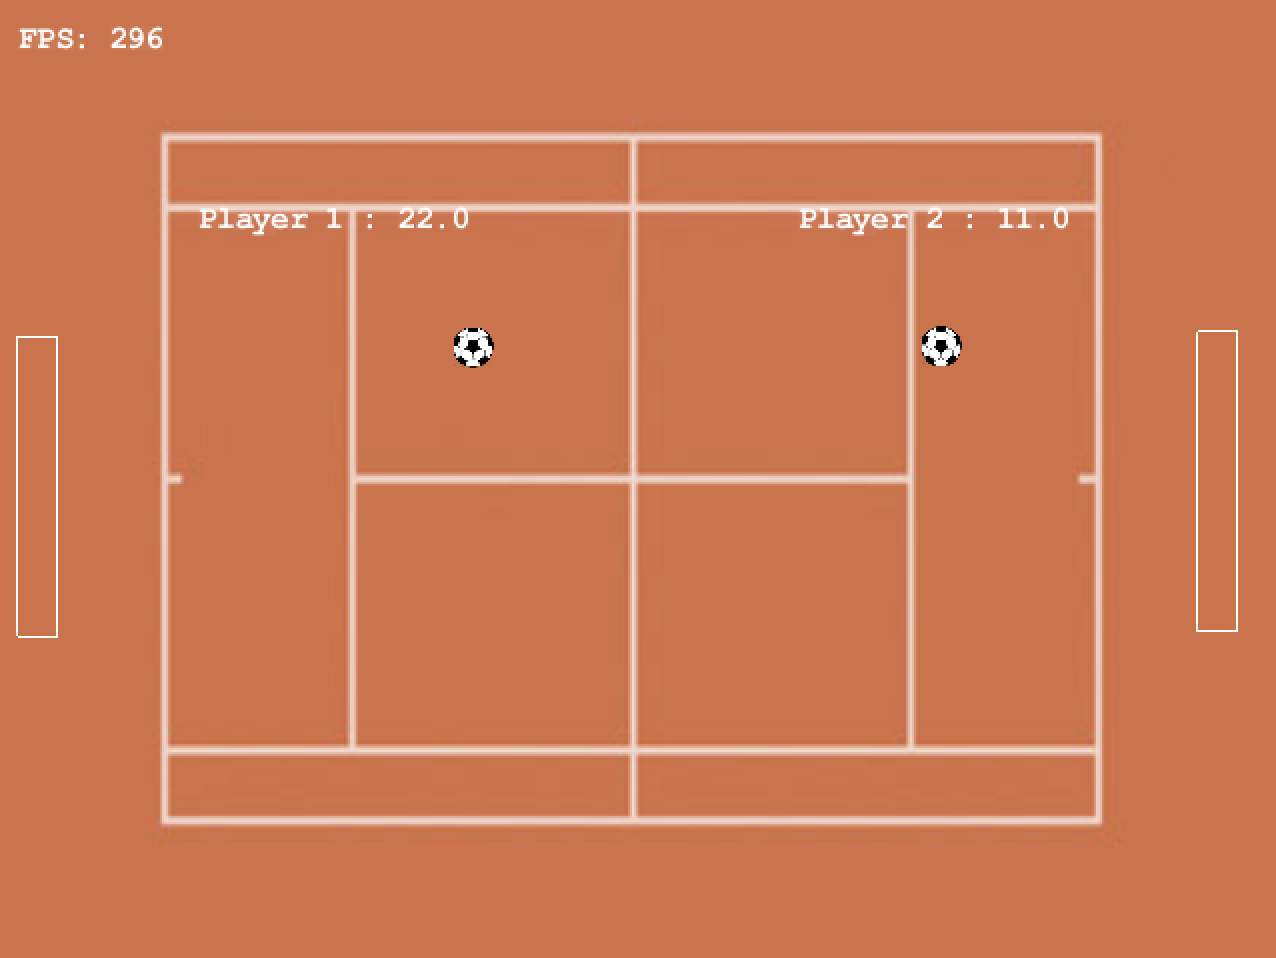
\includegraphics[scale=0.4]{resources/Images/newscreenshot.png}
    \caption{The Ping Pong game as it looked when used for testing.}\label{fig:pingpong}
\end{figure}

\subsubsection{Snake}
The Snake game was used to test the same things as Ping Pong was. Ping Pong was written in around 130 lines, and Snake in about 200 lines. The goal with writing Snake was not to test out different aspects of the language, different from the ones tested in Ping Pong, but to test out the writability of the language.
\pagebreak
\chapter{Reflection}
In this final chapter, the project as a whole is evaluated and some key points are discussed and reflected, with respect to the problem statement. 

\section{Discussion}
In this section, the following points are discussed:

\begin{itemize}
    \item Preliminary analysis
    \item Tennents language design principles
    \item Test
\end{itemize}

These points are discussed to give an insight into the different reflections that the authors of this report has done, and to evaluate some of the decisions made in this project.


\subsection{Preliminary analysis}
The goal of this project was to design and implement a beginner friendly language, and as such, it would have been advantageous if we had done a survey of what knowledge and experience the target audience has in programming and developing software. This could have helped in the design process, since it would have granted some information about what preliminary knowledge the user has.

The language design could have benefited from having an ongoing conversation with either a person with experience in teaching young people, i.e. a teacher, and from tests and surveys performed on the different chosen language structures, all throughout the project. This could have helped in making the design more friendly to use in an educational context, and in improving the overall design, with regards to the main purpose of the language.

The reason for why neither one of these has been done, is that they both were given a lower priority and in the end we had to move on with the project and start implementing the compiler for the language. At this point, it was too late to start on either one, so it was skipped entirely.

\subsection{Tennents language design principles}
Tennents language design principles is a collection of principles that can be very useful when designing a language. These principles are not a strict set of rules, but rather some concepts that should be kept in mind when designing a language. Keeping these principles will help the language being well-designed and easy to understand, as the focus of the rules is to not make any confusing and illogical constructs. There are 3 core principles, as presented in the following sections. 

\subsubsection{Principle of Abstraction}


\subsubsection{Principle of Correspondence}
The principle of correspondence refers to the fact that any declaration, could be turned into a parameter and a corresponding function, as shown here:
\begin{figure}
    \centering
    \begin{lstlisting}[style=gglang]
    num i
    func DoSomething() begin
        set i to 12
    end
    
    //The above corresponds to the below in \lang{}
    
    func DoSomething(num i) begin
    set i to 12
    end
    \end{lstlisting}
    \caption{Principle of correspondence in \lang{}}
    \label{fig:niggers}
Because of this correspondence, the principle of correspondence is kept in \lang{}.
\subsubsection{Principle of Data Type Completeness}
According to Tennents principles, a data type is complete if it is a first class object, without any special restrictions on the use of the object. All data types in \lang{} are first class, and there is no restrictions on how they can be used. Because of this, the principle of Data Type Completeness is kept for \lang{}.

\subsection{Test}
During the implementation phase of the compiler, a corresponding test project was created. In this testing project, different kinds of tests were conducted. These tests covered that the output of the compiler was correct, but did not test any further than that. The testing was limited mainly due to a lack of time, but could easily be expanded to cover the whole compiler project. 

\section{Future work}
The following sections will focus on what could, and should, be done in the future, if \lang{} was ever to be released to the public, and taken into educational use.

\subsubsection{Usability evaluation}
No usability evaluation of \lang{} was conducted during the project. In any future work on \lang{}, it is critical to conduct usability tests on the \lang{} language and compiler and make the necessary corrections to the language. This is needed since the language is meant to as a teaching tool, and must therefore be easy to use. The easy of use can be controlled using these tests.

\subsubsection{IDE}
To help the user when writing games in \lang{}, an IDE should be developed to provide syntax highlighting, auto completion of keywords, game templates to help a user get started, and, in the form of hints, concerning the use of different keywords. A feature, that is missing in the current GUI for using the compiler, is also the possibility to see multiple errors from the lexer/parser phase. As it is at the moment, only 1 error from that phase will be shown at a time, due to limitations in SableCC. This feature could be implemented in future work.\newline
A way of implementing the IDE, in a simple yet effective way, would be to create a plugin for something like notepad \cite{notepad}. This would allow for syntax highlighting, without having to implement a full IDE. 

\subsubsection{Separation of classes}
Providing the ability to separate classes into different text files would provide the user with an easier way to get an overview of the game as a whole. In addition to that, it also makes unit testing easier to implement, and aids maintenance of the code base. 
The concept of separation of classes is a common thing in most programming languages, and as such, it should ideally be implemented into \lang{}.

\subsubsection{Custom libraries}
To make it possible for the user to implement new features in their game, which is not possible in standard \lang{}, it is necessary to allow the user to write custom libraries in either java or \lang{}. This would greatly increase the functionality of \lang{}.
In the current state of \lang{}, it is not possible for the user to implement new libraries, or use libraries written in java. This would be a highly useful feature, and would allow for even better games to be made. As such, it is a goal for future implementations that this is implemented. 

\subsubsection{Community hub}
A sort of community hub, preferably in the form of a forum, for people who wants to use \lang{} to learn about programming, would be an invaluable tool for new users of \lang{}. It would also allow users to share their games, and any custom libraries, they might use. Lastly, it would provide a centralized platform for people seeking help regarding the usage of the \lang{} compiler itself, including a place for reporting any bugs that might appear in the implementation. 
\section{Conclusion}
The goal for this project, as described in the problem statement, was to 

\textit{"Design and develop a beginner friendly programming language that can help to motivate and introduce young people to programming"}

The target audience of the language is young people, who have only had a limited introduction to programming and the different constructs commonly used in programming languages. This is seen in the final design of the language through the different constructs used, such as "downto" and "upto" and by the fact that the language makes use of as few symbols as possible, and instead replaces them with words, such as \textit{begin} and \textit{end}. These design choices are meant to help young people learning programming because they can intuitively understand them. \newline
Another issue was that beginners do not have any experience with IDEs, so a simple GUI was created to allow the user to use the compiler without having to learn how to use complicated IDEs.\newline
The language was made object-oriented, as this is one of the most common programming paradigms used in industries, and since the goal was to introduce them to more common programming structures, object-oriented was a natural choice. It is also easier for the user to map an OOP program to the real world, and vice versa, than it is to map a purely imperative program.\newline
The language focused on having higher readability, rather than focusing on the maintainability and the writability of the language. Readability was the main focus because of the target audience. It was the main goal to make it easier to use and understand what is happening in a piece of code. Writability, especially, suffered because of this, as the high readability imposed a lot of "filler" words in the language in places, where it could have been written with a couple of symbols in many other languages. Maintainability suffered because it takes more work to maintain something in \lang{} due to the added words, but also due to the fact that all classes are written in the same source-file.\newline
The compiler was tested in 2 ways; blackbox and whitebox. Whitebox was done via the test project that was created alongside the compiler project, and it tested if the output of the compiler was correct by comparing it to some expected output. This test covered a wide aspect of the custom constructs used in the language, and as such, it was a good basis for checking whether or not the compiler performed as expected.
Blackbox testing was performed by making a couple of games in the language, and checking what the final game looked like. These are of course not as precise a test as the whitebox tests, but they served as a good indicator for whether or not actual game-making was feasible in \lang{}, which it was. With a very small amount of code, a Ping Pong and a Snake game was made, proving that the language indeed is usable for the intended purpose. 

In the MoSCoW analysis, all the must-have requirements and should-have are implemented. In the could-have category, only the mathematical functions are implemented. Lastly, in the would-have categories, none of the listed features have been implemented. 

The project can be considered successful in the sense that it achieved the goals posed by the problem statement to a sufficient degree of satisfaction.  It is possible to make games using \lang{}, the language itself is easy to read, it is easy to intuitively understand what is going on in a given line of code, it can produce actual games, and it contains constructs that help beginners, who do not have much of an understanding of programming, learn these new constructs. It also met the user-friendliness goal by having a very simple GUI to simplify compilation, and also by not having any requirements in terms of IDE/text editor choice. Of course it can be expanded upon, but as is, the goals of the project were achieved.
\bibliography{bib/mybib}
\label{bib:mybiblio}
\appendix
\chapter{Example program in \lang{}}



\begin{figure}[H]
    \centering
    \begin{lstlisting}[style=gglang]
                                                  /* Could use a global var for points                */
Main begin
  dcl Player player to new Player(20) 
  dcl Ball ball to new Ball(20)
  dcl Enemy enemy to new Enemy(20)
end

class Player is Sprite begin
  dcl num speed

  OnConstruct(num dclspeed) do 
    base(new Point(20, Game.height /2), "/Textures/player.png")
    Game.sprites.add(this)                        /* It adds itself to the pool of active sprites     */            
    set speed to dclspeed
  end

  OnInput(Input key) do                           /* A event as explained in the previous section     */
    if key.IsKeyPress(Key.w) then
      velocity.SetY(-speed)
    else if key.IsKeyPress(Key.s) then
      velocity.SetY(speed)
    else
      velocity.SetY(0)
    end
  end
end



    \end{lstlisting}
\end{figure}

\begin{figure}[H]
    \centering
    \begin{lstlisting}[style=gglang]
class Enemy is Sprite begin
  dcl num speed
  dcl Ball ball

  OnConstruct(num dclspeed) do
    base(new Point(Game.width-20, Game.height /2), "/Textures/enemy.png")
    Game.sprites.add(this)
    set speed to dclspeed
    for i upto Game.sprite.count do               /* Find the ball ball so that we have a reference to it. */
      if Game.sprite.get(i).equal(Ball) then
        set ball to Game.sprite.get(i)            /* This reference is used in OnUpdate */
      end
    end
  end

  funcOnInput(Input key) do                       /* A event as explained in the previous section       */
    if point.y < ball.point.y then                /* Use the reference obtained earlier, to move the enemy accordingly */
      velocity.SetY(speed)
    end
    if point.y > ball.point.y then
      velocity.SetY(-speed)
    end
  end
end

class Ball is Sprite begin
  dcl num speed

  OnConstruct(num dclspeed) do
    base(new Point(Game.width / 2.0, Game.height / 2.0), "/Textures/ball.png")
    Game.sprites.add(this)
    set speed to dclspeed
    dcl num rand to math.GetRandomNum(0, 0.4)     /* Get a random number that will be used as the direction of the ball.*/      
    set velocity to new velocity(1.0-rand, rand)
    set velocity to velocity*speed                /* This is to make the ball move in the start       */           
  end

  OnCollision(sprite other) do
    set speed to speed+1                          /* Make the ball faster every time it hit something */                   
    set velocity to (Vector.Normilise(other.center - center)*speed) 
                                                  /* Make a direction vector and normelise it to move */
                                                  /* from what we hit.                                */
  end

  OnUpdate() do
    if point.y < 0 or point.y > Game.height then 
      velocity.SetY(velocity.y*(-1))               /* Move away from the button and top of the screen  */   
    end
  end
end
    \end{lstlisting}
    \caption{This and the figure above is code for the mini game Ping Pong \label{code:minigame}}
\end{figure}


 \label{ExProg}
\chapter{The full grammar of \lang{}}
Package grammar.ini; \label{FullGrammar}

Helpers
    letter = [['a' .. 'z'] + ['A' .. 'Z']];
    digit = ['0' .. '9'] ;
    tab=9; cr=13; lf=10; space = ' ';

    any = [0..0xffff];



Tokens
    num = 'num';
    bool = 'bool';
    list = 'list';
    text = 'text';
    while = 'while';
    for = 'for';
    begin = 'begin';
    end = 'end';
    do = 'do';
    if = 'if';
    then = 'then';
    else = 'else';
    or = 'or';
    and = 'and';
    set = 'set';
    dcl = 'dcl';
    of = 'of';
    to = 'to';
    new = 'new';
    func = 'func';
    eclass = 'class';
    main = 'Main';
    upto = 'upto';
    downto = 'downto';
    boolval = 'true' | 'false';
    is = 'is';
    comma = ',';
    dot = '.';
    equals = '=';
    notequals = '!=';
    greater = '>';
    less = '<';
    greaterequals = '>=';
    lessequals = '<=';
    not = 'not';
    treturn ='return';
    minus = '-';
    plus = '+';
    divide = '/';
    mult = '*';
    mod = '%';
    lparen = '(';
    rparen = ')';
    numval = digit* ('.' digit*)?;
    newline = (cr | lf | cr lf) (space | (cr | lf | cr lf) | ('/' '*'[any - ['*' + '/']]* '*' '/'))*;
    id = letter(letter|digit)*;
    textval = '"' [any - '"']* '"';
    blank = space*;
    comment = '/' '*'[any - ['*' + '/']]* '*' '/';

Ignored Tokens
     blank,
     comment;

Productions
    prog        {-> prog}   =   global* maindcl newline? classdcl*                      {-> New prog([global.pdcl], maindcl.pdcl, [classdcl.pdcl])};

    global      {-> pdcl}   =   vardcl newline                                          {-> vardcl.pdcl};

    maindcl     {-> pdcl}   =   {maindcl} main begin newline stmt* end           {-> New pdcl.main([stmt.stmt])};

    classdcl    {-> pdcl}   =   {classdcl} [b]:newline eclass id inherit? begin [a]:newline classbody* end    {-> New pdcl.class(id, [classbody.body])};

    classbody   {-> body}   =   {dcl} vardcl newline                                                            {-> New body.class(vardcl.pdcl)}
                            |   {eventdcl} eventdcl newline                                                     {-> New body.eventdcl(eventdcl.pdcl)}
                            |   {funcdcl} dcl func id lparen formalparam? rparen begin funcbody end newline     {-> New body.class(New pdcl.func(id, [formalparam.param], funcbody.body))};

    funcbody    {-> body}   =   newline stmt* return                                    {-> New body.func([stmt.stmt], return.return)};

    return      {-> return} =   {returnid} treturn bexpr newline                        {-> New return.id(bexpr.expr)}
                            |   {empty}                                                 {-> New return.empty()};


    stmt        {-> stmt}   =   {vardcl} vardcl newline                                        {-> New stmt.vardcl(vardcl.pdcl)}
                            |   {assignment} set id to bexpr newline                           {-> New stmt.assignment(id, bexpr.expr)}
                            |   {forup} for id upto bexpr do [a]:newline stmt* end [b]:newline         {-> New stmt.forup(id, bexpr.expr, [stmt.stmt])}
                            |   {fordown} for id downto bexpr do [a]:newline stmt* end [b]:newline     {-> New stmt.fordown(id, bexpr.expr, [stmt.stmt])}
                            |   {while} while bexpr do [a]:newline stmt* end [b]:newline               {-> New stmt.while(bexpr.expr, [stmt.stmt])}
                         //   |   {funccall} funccall newline                                    {-> New stmt.funccall(funccall.call)}
                            |   {classcall} classcall newline                                  {-> New stmt.classcall(classcall.call)}
                            |   {ifstmt} ifstmt newline                                        {-> New stmt.if(ifstmt.conditional)};

    vardcl      {-> pdcl}   =   {vardcl} dcl type id                                    {-> New pdcl.var(type.type, id)}
                            |   {vardclasg} dcl type id to bexpr                        {-> New pdcl.varasg(type.type, id, bexpr.expr)}
                            |   {listdcl} dcl list of type id                           {-> New pdcl.list(type.type, id)};

    ifstmt      {-> conditional} =   if bexpr then newline stmt* elsestmt? end               {-> New conditional.if(bexpr.expr, [stmt.stmt], elsestmt.branch)};

    elsestmt    {-> branch}=   {else} else newline stmt*                              {-> New branch.else([stmt.stmt])}
                             |   {elseif} else if bexpr then newline stmt* elsestmt?    {-> New branch.elseif(bexpr.expr, [stmt.stmt], elsestmt.branch)};


    bexpr       {-> expr}   =   {or} bexpr or bterm                                     {-> New expr.or(bexpr.expr, bterm.expr)}
                            |   {term} bterm                                            {-> bterm.expr};

    bterm       {-> expr}   =   {and} bterm and notfactor                               {-> New expr.and(bterm.expr, notfactor.expr)}
                            |   {factor} notfactor                                      {-> notfactor.expr};

    notfactor   {-> expr}   =   {not} not bfactor                                       {-> New expr.not(bfactor.expr)}
                            |   {factor} bfactor                                        {-> bfactor.expr};

    bfactor     {-> expr}   =   {relation} relation                                     {-> relation.expr};

    relation    {-> expr}   =   {equals} [left]:expression equals [right]:expression                {-> New expr.equals(left.expr, right.expr)}
                            |   {notequals} [left]:expression notequals [right]:expression          {-> New expr.notequals(left.expr, right.expr)}
                            |   {greater} [left]:expression greater [right]:expression              {-> New expr.greater(left.expr, right.expr)}
                            |   {less} [left]:expression less [right]:expression                    {-> New expr.less(left.expr, right.expr)}
                            |   {greaterequals} [left]:expression greaterequals [right]:expression  {-> New expr.greaterequals(left.expr, right.expr)}
                            |   {lessequals} [left]:expression lessequals [right]:expression        {-> New expr.lessequals(left.expr, right.expr)}
                            |   {unarymin} minus expression                                         {-> New expr.unary(expression.expr)}
                            |   {expression} expression                                             {-> expression.expr};

    expression  {-> expr}   =   {minus} [left]:expression minus [right]:term            {-> New expr.minus(left.expr, right.expr)}
                            |   {plus} [left]:expression plus [right]:term              {-> New expr.plus(left.expr, right.expr)}
                            |   {term} term                                             {-> term.expr};

    term        {-> expr}   =   {divide} [left]:term divide [right]:factor              {-> New expr.divide(left.expr, right.expr)}
                            |   {mult} [left]:term mult [right]:factor                  {-> New expr.mult(left.expr, right.expr)}
                            |   {mod} [left]:term mod [right]:factor                    {-> New expr.mod(left.expr, right.expr)}
                            |   {factor} factor                                         {-> factor.expr};

    factor      {-> expr}   =   {value} val                                             {-> New expr.val(val.val)}
                            |   {var} id                                                {-> New expr.id(id)}
                            //|   {func} funccall                                         {-> New expr.call(funccall.call)}
                            |   {classcall} classcall                                   {-> New expr.call(classcall.call)}
                            |   {parenexpr}lparen bexpr rparen                          {-> bexpr.expr};

    type        {-> type}   =   {num} num                                               {-> New type.num(num)}
                            |   {bool} bool                                             {-> New type.bool(bool)}
                            |   {text} text                                             {-> New type.text(text)}
                            |   {object} id                                             {-> New type.object(id)};

    val         {-> val}    =   {numliteral} numval                                     {-> New val.num(numval)}
                            |   {textliteral} textval                                   {-> New val.text(textval)}
                            |   {boolliteral} boolval                                   {-> New val.bool(boolval)}
                            |   {newobject} new id lparen actualparam? rparen           {-> New val.constr(id, [actualparam.expr])};

    funccall    {-> call}   =   {singlefunc} id lparen actualparam? rparen              {-> New call.func(id, [actualparam.expr])};
                    //        |   {nestedfunc} eclass id lparen actualparam? rparen dot funccall {-> New call.funcmulti(id, [actualparam.expr], funccall.call)};

    actualparam {-> expr*}  =   {singleparam} bexpr                                     {-> [bexpr.expr]}
                            |   {mulparam} bexpr comma [rest]:actualparam               {-> [bexpr.expr, rest.expr]};

    formalparam {-> param}  =   {singleparam} type id                                   {-> New param.formal(type.type, id, [])}
                            |   {mulparam} type id comma formalparam                    {-> New param.formal(type.type, id, [formalparam.param])};

    classcall   {-> call}   =   {mulcall} singlecall dot multicall                               {-> New call.class(singlecall.call, [multicall.call])}
                            |   {single} funccall                                       {-> funccall.call};

    singlecall  {-> call}   =   {idcall} id                                             {-> New call.var(id)}
                            |   {funccall} funccall                                     {-> funccall.call};

    multicall   {-> call*}  =   {signle} singlecall                                     {-> [singlecall.call]}
                            |   {multi} singlecall dot [rest]:multicall                 {-> [singlecall.call, rest.call]};

    inherit     {-> inherit}    =    is type                                            {-> New inherit(type)};

    eventdcl    {-> pdcl}  =   id lparen formalparam* rparen do newline [body]:stmt* end          {-> New pdcl.event(id, [formalparam.param], [body.stmt])};


Abstract Syntax Tree

    prog        =   [globaldcl]:pdcl* [maindcl]:pdcl [classdcl]:pdcl*;

    pdcl        =   {var} type id
                |   {varasg} type id expr
                |   {list} type id
                |   {class} id body*
                |   {main} stmt*
                |   {event} id [params]:param* [body]:stmt*
                |   {func} id [params]:param* body;

    body        =   {func} stmt* return
                |   {eventdcl} pdcl
                |   {class} pdcl;

    return      =   {id} expr
                |   {empty} ;

    param       =   {formal} type id param*;

    inherit     =   type;

    type        =   {num} num
                |   {bool} bool
                |   {text} text
                |   {object} id;

    call        =   {func} id [params]:expr*
                |   {class} [first]:call [rest]:call*
                |   {val} val
                |   {var} id;

    expr        =   {minus} [left]:expr [right]:expr
                |   {plus} [left]:expr [right]:expr
                |   {divide} [left]:expr [right]:expr
                |   {mult} [left]:expr [right]:expr
                |   {mod} [left]:expr [right]:expr
                |   {or} [left]:expr [right]:expr
                |   {and} [left]:expr [right]:expr
                |   {equals} [left]:expr [right]:expr
                |   {notequals} [left]:expr [right]:expr
                |   {greater} [left]:expr [right]:expr
                |   {less} [left]:expr [right]:expr
                |   {greaterequals} [left]:expr [right]:expr
                |   {lessequals} [left]:expr [right]:expr
                |   {unary} expr
                |   {not} expr
                |   {val} val
                |   {call} call
                |   {id} id;

    val         =   {num} numval
                |   {text} textval
                |   {bool} boolval
                |   {constr} id [param]:expr*;

    stmt        =   {vardcl} pdcl
                |   {assignment} id expr
                |   {forup} id expr stmt*
                |   {fordown} id expr stmt*
                |   {while} expr stmt*
                |   {if} conditional
                |   {funccall} call
                |   {classcall} call;


    conditional  =   {if} expr stmt* branch?;

    branch      =   {else} stmt*
                |   {elseif} expr stmt* branch?; \label{FGramma}
%\chapter{AST specification of \lang{}}
%Abstract Syntax Tree \label{AST}

    prog        =   [globaldcl]:pdcl* [maindcl]:pdcl [classdcl]:pdcl*;

    pdcl        =   {var} type id
                |   {varasg} type id expr
                |   {list} type id
                |   {class} id body*
                |   {main} body*
                |   {event} id [params]:param* [body]:stmt*
                |   {func} id [params]:param* body;

    body        =   {func} stmt* return
                |   {class} pdcl;

    return      =   {id} expr
                |   {empty} ;

    param       =   {formal} type id param*;

    inherit     =   type;

    type        =   {num} num
                |   {bool} bool
                |   {text} text
                |   {object} id;

    call        =   {func} id [params]:expr*
                |   {class} [first]:call [rest]:call*
                |   {val} val
                |   {var} id;

    expr        =   {minus} [left]:expr [right]:expr
                |   {plus} [left]:expr [right]:expr
                |   {divide} [left]:expr [right]:expr
                |   {mult} [left]:expr [right]:expr
                |   {mod} [left]:expr [right]:expr
                |   {or} [left]:expr [right]:expr
                |   {and} [left]:expr [right]:expr
                |   {equals} [left]:expr [right]:expr
                |   {notequals} [left]:expr [right]:expr
                |   {greater} [left]:expr [right]:expr
                |   {less} [left]:expr [right]:expr
                |   {greaterequals} [left]:expr [right]:expr
                |   {lessequals} [left]:expr [right]:expr
                |   {unary} expr
                |   {not} expr
                |   {val} val
                |   {call} call
                |   {id} id;

    val         =   {num} numval
                |   {text} textval
                |   {bool} boolval
                |   {constr} id [param]:expr*;

    stmt        =   {vardcl} pdcl
                |   {assignment} id expr
                |   {forup} id expr stmt*
                |   {fordown} id expr stmt*
                |   {while} expr stmt*
                |   {if} conditional
                |   {funccall} call
                |   {classcall} call
                |   {eventdcl} pdcl;

    conditional  =   {if} expr stmt* branch?;

    branch      =   {else} stmt*
                |   {elseif} expr stmt* branch?; \label{ASTSpec}
%\chapter{"Pretty" Grammar of \lang{}}
%    prog        =   global* maindcl newline? classdcl*

    global      =   vardcl newline

    maindcl     =   main begin newline stmt* end

    classdcl    =   newline eclass id inherit? begin newline classbody* end

    classbody   =   vardcl newline                                                            
                |   eventdcl newline                                                
                |   dcl func id lparen formalparam? rparen begin funcbody end newline

    funcbody    =   newline stmt* return

    return      =   {returnid} treturn bexpr newline
                |   {empty}                                                 


    stmt        =   vardcl newline                      
                |   set id to bexpr newline               
                |   for id upto bexpr do [a]:newline stmt* end [b]:newline 
                |   for id downto bexpr do [a]:newline stmt* end [b]:newline
                |   while bexpr do [a]:newline stmt* end [b]:newline  
                |   funcdotcall newline         
                |   ifstmt newline                      

    vardcl      =   dcl type id         
                |   dcl type id to bexpr      
                |   dcl list of type id      

    ifstmt      =   if bexpr then newline stmt* elsestmt? end

    elsestmt    =   else newline stmt*
                |   {elseif} else if bexpr then newline stmt* elsestmt?


    bexpr       =   bexpr or bterm             
                |   bterm                   

    bterm       =   bterm and relation 
                |   relation

    relation    =   expression equals expression
                |   expression notequals expression
                |   expression greater expression
                |   expression less expression       
                |   expression greaterequals expression 
                |   expression lessequals expression   
                |   expression 

    expression  =   expression minus term
                |   expression plus term
                |   term


    term        =   term divide [right]:factor  
                |   term mult [right]:factor  
                |   term mod [right]:factor  
                |   unary               

    unary       =   minus factor 
                |   not factor
                |   factor  

    factor      =   val
                |   id
                |   funcdotcall
                |   iddotcall
                |   lparen bexpr rparen

    type        =   num  
                |   bool     
                |   text                        
                |   id   

    val         =   numval
                |   textval
                |   boolval
                |   this
                |   new id lparen actualparam? rparen

    funccall    =   id lparen actualparam? rparen


    actualparam =   bexpr
                |   bexpr comma actualparam

    formalparam {-> param*}  =   {singleparam} type id                                  {-> [New param.formal(type.type, id)]}
                            |   {mulparam} type id comma formalparam                    {-> [New param.formal(type.type, id), formalparam.param]};

    funcdotcall {-> call}   =   {mulcall} singlecall dot multicallfunc                  {-> New call.dot(singlecall.call, [multicallfunc.call])}
                            |   {single} funccall                                       {-> funccall.call};

    iddotcall {-> call}     =   {mulcall} singlecall dot multicallid                    {-> New call.dot(singlecall.call, [multicallid.call])};

    singlecall  {-> call}   =   {idcall} id                                             {-> New call.var(id)}
                            |   {funccall} funccall                                     {-> funccall.call};

    multicallid {-> call*}  =   {single} id                                             {-> [New call.var(id)]}
                            |   {multi} singlecall dot [rest]:multicallid                 {-> [singlecall.call, rest.call]};

    multicallfunc   {-> call*}  =   {single} funccall                                   {-> [funccall.call]}
                                |   {multi} singlecall dot [rest]:multicallfunc             {-> [singlecall.call, rest.call]};


    inherit     {-> inherit}    =    is type                                            {-> New inherit(type)};

    eventdcl    {-> pdcl}   =   id lparen formalparam* rparen do newline baseconstr? [body]:stmt* end          {-> New pdcl.event(id, [formalparam.param], baseconstr.base, [body.stmt])};

    baseconstr  {-> base}   =   tbase lparen actualparam? rparen newline                {-> New base.base([actualparam.expr])}; \label{PGramma}
%\chapter{Source for PingPong}
%dcl num score1 to 0
dcl num score2 to 0
dcl Ball ball to new Ball()

Main begin
    dcl Player player to new Player()
    dcl Enemy enemy to new Enemy()

    dcl num h to 1
    for h upto 2 do
        set ball to new Ball()
    end

    game.SetBackground("Resources/arena.png")
end

class Player is Sprite begin
    dcl num speed
    dcl num vel

    dcl Label p1 to new Label("Player 1 : " + score1, 100, 100)

    OnConstruct() do
        base(10, 200, 100, 150, "Player")
        set speed to 200
        set texture to "Resources/redfighter0006.png"
        game.Sprites.add(this)
    end

    OnUpdate(num delta) do
        if input.key.W.isDown then
             set vel to -speed
        else if input.key.S.isDown then
             set vel to speed
        else
            set vel to 0
        end
        set posY to posY+vel * (delta / 1000)

        if posY < ball.posY then                /* Use the reference obtained earlier, to move the enemy accordingly */
              set vel to speed

            else if posY > ball.posY then
              set vel to -speed
        end
        set posY to posY+vel  * (delta / 1000)

        p1.updateText("Player 1 : " + score1)
    end
end

class Enemy is Sprite begin
  dcl num speed to 100
  dcl num vel
  dcl Label p2 to new Label("Player 2 : " + score2, 400, 100)

  OnConstruct() do
    base(600, 100, 20, 150, "Enemy")
    game.Sprites.add(this)
  end

  OnUpdate(num delta) do                           /* A event as explained in the previous section       */
    if posY < ball.posY then                /* Use the reference obtained earlier, to move the enemy accordingly */
      set vel to speed

    else if posY > ball.posY then
      set vel to -speed
    end
    set posY to posY+vel  * (delta / 1000)
    p2.updateText("Player 2 : " + score2)
  end



end

class Ball is Sprite begin
  dcl num speed
  dcl num yspeed
  dcl num xspeed
  dcl num dir


  OnConstruct() do
    base(200, 200, 20,20, "Ball")
    set texture to "Resources/pokeball.png"

    set speed to 300
    set xspeed to speed
    game.Sprites.add(this)
  end

  OnCollision(Sprite other) do
        if not (other.id = "Ball") then
            set xspeed to -xspeed
            set dir to math.getRandomNum(200) + 50

            if dir = 1 then
                set yspeed to dir
            else
                set yspeed to -dir
            end
        end

  end

  OnUpdate(num delta) do


    if posY <= 0 then
       set yspeed to -yspeed
    else if posY >= 480 then
       set yspeed to -yspeed
    end

    if posX <= 0 then
        set score2 to score2 + 1
        set posX to 320
    end

    if posX >= 640 then
        set score1 to score1 + 1
        set posX to 320
    end

    set posY to posY + yspeed * (delta / 1000)
    set posX to posX + xspeed * (delta / 1000)


  end
end \label{sourcepingpong}
\end{document}